% PhD thesis template, Lund University
% Originally designed for the Faculty of Science: Astronomy and Theoretical Physics
% Reformatted to work with Overleaf

% Layout and typesetting: Daniel Michalik, with Berry Holl, Helene Jönsson, Jonas Palm, Samuel Stenberg, Vidar Aspelin
% Implementation and documentation: Daniel Michalik, Samuel Stenberg
%
% Credits to the past generations of students who contributed to the original
% versions of this latex template, in particular Berry Holl.
% 
% Compilation instructions: use "xelatex" (necessary for support of the fonts
% used by Lund University. The fonts need to be installed first, see README.txt
% for instructions).
%
% If you use (pdf)latex instead, the default latex fonts will be used. 
% That would be a pity, cause the Garamond/Frutiger suggestion by the
% University looks much nicer for your thesis!
%
% Special command to automatically make Mac's TeXshop use xelatex for this file:
% !TEX TS-program = XeLaTeX
%
\documentclass[11pt]{book} 

% Hide all the usepackage commands and definitions in a preamble file.
% Normally you should not need to edit it.

% Custom aliases
%\newcommand{\jpsi}{\rm J/$\psi$}
%\newcommand{\psip}{$\psi^\prime$}
%\newcommand{\jpsiDY}{\rm J/$\psi$\,/\,DY}
%\newcommand{\dd}{\mathrm{d}}
%\newcommand{\chic}{$\chi_{\rm c}$}
%\newcommand{\ezdc}{$E_{\rm ZDC}$}
%\newcommand{\red}{\textcolor{red}}
%\newcommand{\blue}{\textcolor{blue}}
\newcommand{\RT}{\ensuremath{R_{\rm T}}\xspace}
\newcommand{\RTmin}{\ensuremath{R_{\rm T,min}}\xspace}
\newcommand{\RTmax}{\ensuremath{R_{\rm T,max}}\xspace}
\newcommand{\NT}{\ensuremath{N_{\rm T}}\xspace}
\newcommand{\NTmin}{\ensuremath{N_{\rm T,min}}\xspace}
\newcommand{\NTmax}{\ensuremath{N_{\rm T,max}}\xspace}
\newcommand{\NTt}{\ensuremath{N_{\rm T}^{t}}\xspace}
\newcommand{\NTtt}{\ensuremath{N_{\rm T}^{t'}}\xspace}
\newcommand{\NTm}{\ensuremath{N_{\rm T}^{m}}\xspace}
\newcommand{\nevhat}{\ensuremath{\hat{n}_{\rm ev}}\xspace}
\newcommand{\nev}{\ensuremath{n_{\rm ev}}\xspace}

\newcommand{\ptlead}{\ensuremath{p_{\rm T}^{\rm leading}}\xspace}
\newcommand{\philead}{\ensuremath{\phi^{\rm leading}}\xspace}
\newcommand{\meannmpi}{\ensuremath{\langle n_{\rm MPI} \rangle}\xspace}
\newcommand{\nmpi}{\ensuremath{n_{\rm MPI}}\xspace}
\newcommand{\tracklet}{\ensuremath{N_{\text{tracklets}}^{\text{$|\eta| < 0.8$}}}\xspace}
\newcommand{\INELgtO}{\ensuremath{\text{INEL} > 0}\xspace}
\newcommand{\dndy}         {\ensuremath{\mathrm{d}N_\mathrm{ch}/\mathrm{d}y}\xspace}
\newcommand{\dndeta}       {\ensuremath{\mathrm{d}N_\mathrm{ch}/\mathrm{d}\eta}\xspace}
\newcommand{\myield}       {\ensuremath{\left<\mathrm{d}N/\mathrm{d}y\right>}\xspace}
\newcommand{\myieldpi}       {\ensuremath{\left<\mathrm{d}N_\mathrm{\pi}/\mathrm{d}y\right>}\xspace}

\newcommand{\avdndeta}     {\ensuremath{\langle\dndeta\rangle}\xspace}
\newcommand{\Npart}        {\ensuremath{N_\mathrm{part}}\xspace}
\newcommand{\Ncoll}        {\ensuremath{N_\mathrm{coll}}\xspace}

\newcommand{\Raa}{\ensuremath{\rm R_{AA}}\xspace}
\newcommand{\Rpa}{\ensuremath{\rm R_{pA}}\xspace}
\newcommand{\Rppb}{\ensuremath{R_{\rm pPb}}\xspace}

\newcommand{\cme}{\ensuremath{\sqrt{s}}\xspace}
\newcommand{\gev}{\ensuremath{{\rm GeV}/c}\xspace}
\newcommand{\auau}{\ensuremath{\rm Au\!-\!Au}\xspace}
%\newcommand{\ptopi}{\ensuremath{({\rm p+ \bar{p}}) / (\pi^{+}+\pi^{-})}\xspace}
\newcommand{\pikp}{\ensuremath{\pi/{\rm K}/{\rm p}}\xspace}
\newcommand{\ptopi}{\ensuremath{{\rm p } / \pi}\xspace}
\newcommand{\ktopi}{\ensuremath{({\rm K}^{+}+{\rm K}^{-}) / (\pi^{+}+\pi^{-})}\xspace}
\newcommand{\twotwo}{\ensuremath{2\rightarrow 2}\xspace}
\newcommand{\ltok}{\ensuremath{({\rm \Lambda}^{0}+\bar {\rm \Lambda}^{0})/(\rm 2 K^{0}_{s} )} \xspace}

\newcommand{\snng}[1]{\ensuremath{\sqrt{s_{\rm NN}} = #1 \text{\,GeV}}\xspace}
\newcommand{\snnt}[1]{\ensuremath{\sqrt{s_{\rm NN}} = #1 \text{\,TeV}}\xspace}
% \newcommand{\snnt}[1]{\ensuremath{\sqrt{s_{NN}} = #1 \text{ TeV}}\xspace}
\newcommand{\snnnotext}[1]{\ensuremath{\sqrt{s_{NN}} = #1}\xspace}
\newcommand{\sppt}[1]{\ensuremath{\sqrt{s} = #1 \text{\,TeV}}\xspace}
\newcommand{\sppg}[1]{\ensuremath{\sqrt{s} = #1 \text{\,GeV}}\xspace}
\newcommand{\gevc}[1]{\ensuremath{#1 \text{\,GeV/$c$}}\xspace}
\newcommand{\mevc}[1]{\ensuremath{#1 \text{\,MeV/$c$}}\xspace}
\newcommand{\gevcc}[1]{\ensuremath{#1 \text{\,GeV/$c^2$}}\xspace}
\newcommand{\mevcc}[1]{\ensuremath{#1 \text{\,MeV/$c^2$}}\xspace}
\newcommand{\eff}[1]{\ensuremath{\epsilon_{#1}}\xspace}
\newcommand{\bareyield}{\ensuremath{Y}\xspace}
\newcommand{\yield}[1]{\ensuremath{Y_{#1}}\xspace}
\newcommand{\ch}{\ensuremath{\text{ch}}\xspace}
\newcommand{\etalab}{\ensuremath{\eta_{lab}}\xspace}
\newcommand{\cmc}[1]{\ensuremath{#1 \text{\,cm/$c$}}\xspace}

\newcommand{\VZ}{\ensuremath{V^{0}}\xspace}
\newcommand{\VZs}{\ensuremath{V^{0}\text{s}}\xspace}
\newcommand{\RAA}{\ensuremath{R_{\text{AA}}}\xspace}
\newcommand{\MRAA}{\ensuremath{\mathbf{R_{\text{\textbf{AA}}}}}\xspace}
%\newcommand{\ppb}{\ensuremath{\rm p\!-\!Pb}\xspace}
%\newcommand{\pbpb}{\ensuremath{\rm Pb\!-\!Pb}\xspace}
\newcommand{\pp}{pp\xspace}
\newcommand{\ppb}{p--Pb\xspace}
\newcommand{\pbpb}{Pb--Pb\xspace}
\newcommand{\pim}{\ensuremath{\pi^{-}}\xspace}
\newcommand{\pip}{\ensuremath{\pi^{+}}\xspace}
\newcommand{\km}{\ensuremath{K^{-}}\xspace}
\newcommand{\kp}{\ensuremath{K^{+}}\xspace}
\newcommand{\kpm}{\ensuremath{K^{\pm}}\xspace}
\newcommand{\p}{\ensuremath{p}\xspace}
\newcommand{\pbar}{\ensuremath{\bar{p}}\xspace}
\newcommand{\mathpt}{\ensuremath{\mathbf{p_{\text{T}}}}\xspace}
\newcommand{\pt}{\ensuremath{p_{\text{T}}}\xspace}
\newcommand{\dpi}{\ensuremath{\Delta_{\pi}}\xspace}
\newcommand{\dkaon}{\ensuremath{\Delta_{K}}\xspace}
\newcommand{\dproton}{\ensuremath{\Delta_{p}}\xspace}
\newcommand{\mdpi}{\ensuremath{\mathbf{\Delta_{\pi}}}\xspace}
\newcommand{\mdkaon}{\ensuremath{\mathbf{\Delta_{K}}}\xspace}
\newcommand{\mdproton}{\ensuremath{\mathbf{\Delta_{p}}}\xspace}
\newcommand{\rpi}{\ensuremath{R_{\pi}}\xspace}
\newcommand{\mathdedx}{\ensuremath{\mathbf{\text{d}E/\text{d}x}}\xspace}
\newcommand{\dedx}{\ensuremath{\text{d}E/\text{d}x}\xspace}
\newcommand{\mdedx}{\ensuremath{\left <\text{d}E/\text{d}x \right>}\xspace}
\newcommand{\mathmdedx}{\ensuremath{\mathbf{\left <\text{d}E/\text{d}x \right>}}\xspace}
\newcommand{\mdedxpi}{\ensuremath{\left <\text{d}E/\text{d}x \right>_{\pi}}\xspace}
\newcommand{\meanp}{\ensuremath{\langle p \rangle}\xspace}
\newcommand{\meanpt}{\ensuremath{\langle \pt \rangle}\xspace}
\newcommand{\sdedx}{\ensuremath{\sigma_{\text{d}E/\text{d}x}}\xspace}
\newcommand{\relres}{\ensuremath{\sigma/\left <\text{d}E/\text{d}x \right>}\xspace}
\newcommand{\res}{\ensuremath{\sigma_{\text{d}E/\text{d}x}}\xspace}
% \newcommand{\relres}{\ensuremath{\sigma/\left <\text{d}E/\text{d}x \right>\xspace}
\newcommand{\ncl}{\ensuremath{\text{Ncl}}\xspace}
\newcommand{\mncl}{\ensuremath{\langle \text{Ncl} \rangle}\xspace}

\newcommand{\chpi}{\ensuremath{\pi^{+}+\pi^{-}}\xspace}
\newcommand{\chk}{\ensuremath{{\rm K}^{+}+{\rm K}^{-}}\xspace}
\newcommand{\chp}{\ensuremath{{\rm p}+{\rm \bar{p}}}\xspace}

\newcommand{\bg}{\ensuremath{\beta\gamma}\xspace}

\newcommand{\VOA}{\ensuremath{\rm V 0 \rm A}\xspace}
\newcommand{\VOC}{\ensuremath{\rm V 0 \rm C}\xspace}
\newcommand{\VOM}{\ensuremath{\rm V 0 \rm M}\xspace}
\newcommand{\VO}{\ensuremath{\rm V^0}\xspace}
\newcommand{\VOs}{\ensuremath{\rm V^0 s}\xspace}

\newcommand{\LA}{\ensuremath{\Lambda}\xspace}
\newcommand{\AL}{\ensuremath{\overline{\Lambda}}\xspace}
\newcommand{\KOs}{\ensuremath{\rm{K^0_S}}\xspace}
\newcommand{\dMassG}{\ensuremath{\Delta m_\gamma}\xspace}
\newcommand{\dMassL}{\ensuremath{\Delta m_\Lambda}\xspace}
\newcommand{\dMassAL}{\ensuremath{\Delta m_{\bar{\Lambda}}}\xspace}
\newcommand{\dMassKO}{\ensuremath{\Delta m_{K^0_s}}\xspace}
\newcommand{\dMassVO}{\ensuremath{\Delta m_{\rm V 0}}\xspace}

\newcommand{\Ks}{\ensuremath{\rm K^0_S}\xspace}
\newcommand{\dMassKs}{\ensuremath{\Delta m_{K^0_s}}\xspace}
\newcommand{\MVO}{\ensuremath{M_{\rm V 0}}\xspace}

\newcommand{\XI}{\ensuremath{\Xi}\xspace}
\newcommand{\PI}{\ensuremath{\pi}\xspace}
\newcommand{\XIM}{\ensuremath{\Xi^-}\xspace}
\newcommand{\XIP}{\ensuremath{\overline{\Xi}^+}\xspace}
\newcommand{\XISUM}{\ensuremath{\Xi^-+\bar{\Xi}^+}\xspace}
\newcommand{\Nch}{\ensuremath{N_{\text{ch}}}\xspace}
\newcommand{\meanNch}{\ensuremath{\langle N_{\text{ch}} \rangle}\xspace}
\newcommand{\Ntracks}{\ensuremath{N_{\text{tracks}}}\xspace}
\newcommand{\Minv}{\ensuremath{M_{\text{inv}}}\xspace}
\newcommand{\SO}{\ensuremath{S_{\text{O}}}\xspace}
\newcommand{\TrkRec}{\ensuremath{\textrm{Trk}_{\textrm{Rec}}}\xspace}
\newcommand{\TrkGen}{\ensuremath{\textrm{Trk}_{\textrm{Gen}}}\xspace}
\newcommand{\SORec}{\ensuremath{S_{\text{O}_{\textrm{Rec}}}^{(\pt = 1.0)}}\xspace}
\newcommand{\SOGen}{\ensuremath{S_{\text{O}_{\textrm{Gen}}}^{(\pt = 1.0)}}\xspace}

\newcommand{\SOPT}{\ensuremath{S_{\text{O}}^{(\pt = 1.0)}}\xspace}
\newcommand{\nsigma}{\ensuremath{n\sigma}\xspace}
\newcommand{\NSPD}{\ensuremath{N_{{\textrm{SPD}}_{\textrm{Trklts}}}}\xspace} 
\newcommand{\NSIGMAKTPC}{\ensuremath{n\sigma_{\rm K}^{\rm TPC}}\xspace}
\newcommand{\NSIGMAKTOF}{\ensuremath{n\sigma_{\rm K}^{\rm TOF}}\xspace}

\newcommand{\Gaus}{\ensuremath{\mathcal{N}}\xspace}
\newcommand{\Chisq}{\ensuremath{\chi^2}\xspace}


% Non-breakable hyphen. Use for things like "(re-)print". 
\newcommand\nobrkhyph{\mbox{-}}

% Small caps serif font, for Paper numbers, ISBN, etc
\newcommand{\I}{\textrm{\scshape i}\xspace}
\newcommand{\II}{\textrm{\scshape ii}\xspace}
\newcommand{\III}{\textrm{\scshape iii}\xspace}
\newcommand{\IV}{\textrm{\scshape iv}\xspace}
\newcommand{\V}{\textrm{\scshape v}\xspace}
\newcommand{\VI}{\textrm{\scshape vi}\xspace}
\newcommand{\VII}{\textrm{\scshape vii}\xspace}
\newcommand{\VIII}{\textrm{\scshape viii}\xspace}
\newcommand{\IX}{\textrm{\scshape ix}\xspace}
\newcommand{\X}{\textrm{\scshape x}\xspace}
\newcommand{\ISBN}{\textrm{\scshape isbn}\xspace}
\newcommand{\ISSN}{\textrm{\scshape issn}\xspace}

% Must come in the beginning. Changes the spacing in the table of contents to look more pleasing
\usepackage{tocloft}
\setlength{\cftbeforepartskip}{5.0mm}
\setlength{\cftbeforechapskip}{2.0mm}
\setlength{\cftbeforesecskip}{0.0mm}

% Must come in the beginning. To calculate the total number of pages
\usepackage{pageslts}

%%%%%%%%%%%%%%%%%%%%%%%%%% Everything font-related %%%%%%%%%%%%%%%%%%%%%%%%%%%%%%%%%%%%%%%
\usepackage{ifxetex}

% Font selections - they are only used when you compile with xelatex (strongly recommended). If you use 
% pdflatex, the default latex fonts will be used, you will break the University graphical profile, and your
% thesis will look much much uglier.
%\usepackage[adobe-garamond]{mathdesign}
\ifxetex
	\usepackage{mathspec}
	\usepackage[no-math]{fontspec}
	\usepackage{xunicode}
	\usepackage{xltxtra}
    %\usepackage[adobe-garamond]{mathdesign}
    \usepackage[Adobe Garamond]{mathdesign}
	% Adobe Garamond Pro for serif fonts and maths, Frutiger as sans, according to LU graphical profile
	% Tables get monospaced numerals, text gets proportional numerals, mathmode gets uppercase monospaced numberals
	%\setmainfont[Mapping=tex-text,Numbers={OldStyle,Proportional}]{Adobe Garamond Pro}
	\setmainfont{AGaramondPro}[Path = ./fonts/AGaramondPro/, Mapping = tex-text, Numbers = {OldStyle, Proportional}, UprightFont = *-Regular.otf, BoldFont= *-Semibold.otf, ItalicFont=*-Italic.otf]
	\AtBeginEnvironment{tabular}{\addfontfeatures{Numbers={Monospaced}}}
	%\setsansfont{Frutiger LT Std 45 Light}
	%\setsansfont{FrutigerLTStd}[Path = ./fonts/Frutiger/, RomanFont=*-Roman.otf, BoldFont=*-Bold.otf, ItalicFont=*-Italic.otf, LightFont=*-Light.otf, LightItalicFont=*-LightItalic.otf]
	\setsansfont{FrutigerLTStd-Roman.ttf}[Path = ./fonts/Frutiger/, BoldFont=FrutigerLTStd-Bold.ttf, ItalicFont=FrutigerLTStd-Italic.ttf]
	
	%\setmathfont(Greek,Digits,Latin){Adobe Garamond Pro}
	%\setmathfont(Greek,Digits,Latin){AGaramondPro-Roman.otf}
	% mathspec is broken. The next eight lines work around that.
	\usepackage{etoolbox}
	\makeatletter
	\begingroup\lccode`~=`"
	\lowercase{\endgroup
	  \everymath{\let~\eu@active@quote}
	  \everydisplay{\let~\eu@active@quote}
	}
	\makeatother
\else
	% This is what is used for pdf latex. 
	% You can try \usepackage{ebgaramond} with (pdf)latex, however that does not have bold fonts ... !
	%\usepackage{ebgaramond}
	 \usepackage[utf8]{inputenc}
\fi
%%%%%%%%%%%% end font selections

% Support for greek (non-math non-italic) text, e.g. for units like mircometer: \textmu m 
\usepackage{textgreek}

% Additional font sizes \HUGE and \ssmall, needed for figure captions
\usepackage{moresize}

% figure captions in bold (i.e. "Figure 1" in bold), sans serif, smaller font size, hanging label, always starting on the left side
\usepackage{subfig}
\DeclareCaptionFont{ssmall}{\ssmall}
\DeclareCaptionFont{tiny}{\tiny}% "scriptsize" is defined by floatrow, "tiny" not
\captionsetup{margin=0em,font={ssmall,sf},labelfont={bf},format=hang,singlelinecheck=false} 
%centering subcaptions
\captionsetup[subfloat]{justification=centering} 

% figures centred, smaller font in tables, captions on top for tables
\usepackage{floatrow}
\DeclareFloatFont{tiny}{\tiny}% "scriptsize" is defined by floatrow, "tiny" not
\DeclareFloatFont{ssmall}{\ssmall}
\floatsetup[table]{font={footnotesize},position=top}
%%%%%%%%%%%%%%%%%%%%%%%%%%%%%%%%%%%% end fonts %%%%%%%%%%%%%%%%%%%%%%%%%%%%%%%%%%%%%%%%%%%%%%%%%%%%%%%

% For tables spanning the full text width
\usepackage{tabularx}

% For fat greek letters in math mode
\usepackage{bm}

% for diagrams
\usepackage{tikz}
\usepackage[compat=1.1.0]{tikz-feynman}
\usetikzlibrary{positioning, arrows.meta, bending, fit, calc, decorations.pathmorphing}

%for cropping pictures
\usepackage{adjustbox}

% For URLs use \url{<URL>}
\usepackage{url}

% For clickable references and citations
\usepackage[hidelinks]{hyperref}


% Chapters should have numbers - a typical thesis consists of two chapters:
% One to introduce and summarize the research ("kappa"), and one for
% reproductions of the papers and manuscripts. No need to number them by default.
% If you need chapter numbers back, comment the following line.
%\renewcommand{\thesection}{\arabic{section}} 

% Sections and subsections have numbers, subsubsections etc do not.
\setcounter{secnumdepth}{3}

% Only chapters and sections appear in the table of contents, not subsections etc
\addtocontents{toc}{\protect\setcounter{tocdepth}{3}}

% Ensures that \cleardoublepage inserts empty pages without page number
\usepackage{emptypage} 

% For text macros (e.g., small caps macros)
\usepackage{xspace}

% For "Lorem Ipsum" style place holders
\usepackage{blindtext}

% For \includegraphics
\usepackage{graphicx}


% Nice looking tables with correct spacings 
\usepackage{booktabs}

% Tables spanning more than one page
\usepackage{longtable}
 
% Math symbols
\usepackage{amsfonts,mathrsfs,amsmath,amssymb}
\usepackage[ruled,vlined]{algorithm2e}
% To include the PDFs of the papers
\usepackage{pdfpages}

% Easier equations
\usepackage{derivative}

% For inline verbatim
\usepackage{spverbatim}

% For subfigures
%\usepackage{caption}
%\usepackage{subcaption}

% For slash notation
\usepackage{slashed}

% For Natural Science students who use ADS. Save to have in any case.
\usepackage{auxiliary_textfiles/aas_macros}

% Hyphenation, support for different languages, last one is default
% Make sure to install the hyphenation packages for all languages you need
\usepackage[swedish,ngerman,english]{babel} 

% Reference in style of Natural Sciences
\usepackage[square, numbers, comma, sort]{natbib}

% Command to edit the IEEE style
\makeatletter
\def\bstctlcite{\@ifnextchar[{\@bstctlcite}{\@bstctlcite[@auxout]}}
\def\@bstctlcite[#1]#2{\@bsphack
  \@for\@citeb:=#2\do{%
    \edef\@citeb{\expandafter\@firstofone\@citeb}%
    \if@filesw\immediate\write\csname #1\endcsname{\string\citation{\@citeb}}\fi}%
  \@esphack}
\makeatother 

% Non-indented paragraphs with a small vertical space in-between
\parindent 0in
\parskip 3mm

% Paper size. Typically this works also fine when printed on A4 (text size is
% as print later, just the margins become wider to accommodate the too large
% sheets).
%% G5 format
%\usepackage[paperwidth=169mm,paperheight=239mm,total={13.3cm,19.6cm}, top=1.8cm, ignorehead, centering, footskip=\footskip+4mm ]{geometry}
\usepackage[paperwidth=169mm,paperheight=239mm,total={12.5cm,19.6cm}, top=1.8cm, ignorehead, centering, footskip=\footskip+4mm ]{geometry}
% If you prefer E5 (smaller) you can use this line instead. Also go to frontmatter.tex and change the datasheet from G5 to E5.
%% E5 format
%\usepackage[paperwidth=155mm,paperheight=220mm,total={12cm,18cm}, top=1.8cm, ignorehead, centering, footskip=\footskip+4mm ]{geometry}

% not every page needs to go to the same bottom line. Allows nicer page breaks.
\raggedbottom

% avoid orphan/widow lines. Lower this number if necessary to get a good layout.
\widowpenalty500
\clubpenalty500


% These command should allow figures to be placed close to where we define them, 
% thus we can influence the figure placement to some extent.
%% min page fraction that must be filled with text
%\renewcommand{\textfraction}{0.1} 
\renewcommand{\textfraction}{0.2}
%% max page fraction that a float may take at the top of the page
%\renewcommand{\topfraction}{0.9} 
\renewcommand{\topfraction}{1.0}
%% max page fraction that a float may take at the bottom of the page
%\renewcommand{\bottomfraction}{0.9}
\renewcommand{\bottomfraction}{1.0}
%% max page fraction that may be filled with floats
%\renewcommand{\floatpagefraction}{0.5}
\renewcommand{\floatpagefraction}{1.0}
%% maximum number of floats at the top of the page
\setcounter{topnumber}{1}
%% maximum number of floats at the bottom of the page
\setcounter{bottomnumber}{1}
%% maximum total number of floats on a page
\setcounter{totalnumber}{1}

% Figures can be kept in the same directory as the thesis, or in a Figure/
% directory, without need to specifying which of the two it is
\graphicspath{{figures/}}


%%%%%%%%%%%%%%%%%%%%%%%%%%%%%%%%%%%%%%%%%%%%%%%%%%%%%%%%%%%%%%%%%%%%
% define commands for chapters, sections, and subsections that do not 
% have a number, but are entered as candidates for the table of contents.
\newcommand\chap[1]{%
  \chapter*{#1}%
  \addcontentsline{toc}{chapter}{#1}
  \markboth{#1}{#1}
}
\newcommand\sect[1]{%
  \section*{#1}%
  \addcontentsline{toc}{section}{#1}
  \markright{#1}
}
\newcommand\subsect[1]{%
  \subsection*{#1}%
  \addcontentsline{toc}{subsection}{#1}
}
\newcommand\subsubsect[1]{%
  \subsubsection*{#1}%
  \addcontentsline{toc}{subsubsection}{#1}
}


%%%%%%%%%%%%%%%%%%%%%%%%%%%%%%%%%%%%%%%%%%%%%%%%%%%%%%%%%%%%%%%%%%%%
% Define nice headers and footers
% To keep the thesis non-cluttered we only put the page number into the footer,
% and avoid headers
\usepackage{fancyhdr}
\fancyheadoffset{0cm}
\pagestyle{plain}
%page number in the foot centre 
\cfoot{\fancyplain{\thepage}{}}

% You want to use headers? Here is some things for your inspiration:
%\renewcommand{\chaptermark}[1]%
%               {\markboth{#1}{#1}}
%\renewcommand{\sectionmark}[1]%
%               {\markright{\thesection\ #1}}
%\renewcommand{\chaptermark}[1]{\markboth{\thechapter\ #1}{\thechapter\ #1}}
%\lhead[\fancyplain{}{\thepage}]%
%      {\fancyplain{}{\textsl\rightmark}}
%\rhead[\fancyplain{}{\textsl\leftmark}]%
%      {\fancyplain{}{\thepage}}
% Contents and references should not print a uppercase header on their second pages
%\usepackage{etoolbox}
%\patchcmd{\tableofcontents}{\MakeUppercase\contentsname}{\contentsname}{}{}
%\patchcmd{\tableofcontents}{\MakeUppercase\contentsname}{\contentsname}{}{}
%\patchcmd{\bibsection}{\MakeUppercase{\bibname}}{\bibname}{}{}
%\patchcmd{\bibsection}{\MakeUppercase{\bibname}}{\bibname}{}{}

% References should be a section of the summary text, with number and all ...
\renewcommand\bibsection{\chap{\bibname}\markright{\bibname}}

% If you want to use a box to summarize your papers, try \begin{thesisbox}{title}
\usepackage{tcolorbox}
\tcbuselibrary{skins}
\newtcolorbox{thesisbox}[2][]{
oversize=-2.5cm,
  enhanced,
  attach boxed title to top left={yshift=-2ex,xshift=6ex},
  before skip=1em,
  after skip=1em,
  colframe=black,
  colback=white,
  fonttitle=\bfseries, 
  colbacktitle=white,
  coltitle=black,
  boxed title style={
    boxrule=0pt,
    colframe=white,
    },
  title=#2,
  #1}
\newcounter{exa}

% ********************************************************************
% Re-usable information (title page, datasheet), please edit the file parameters.tex to include correct information
\newcommand{\myName}{Oliver Matonoha}
\newcommand{\myYear}{2023}
\newcommand{\myMainTitle}{Production of strangeness in partonic interactions at the LHC}
\newcommand{\mySubTitle}{}

% Compact combination of combining title and subtitle, used in datasheet and as
% chapter title for the main part.
\newcommand{\myTitle}{\myMainTitle\ \mySubTitle} 

\newcommand{\myFaculty}{Faculty of Natural Sciences}
\newcommand{\myDepartment}{Department of Physics}
\newcommand{\myAddress}{Box 124\\SE--221 00 LUND\\Sweden} % Three lines maximum!

% Only change once you are ready. Looks to scary otherwise.
% This might be the degree you are obtaining: Thesis for the degree of Doctor of Philosophy
\newcommand{\myDegree}{Thesis for the degree of Doctorate}
\newcommand{\myAdvisors}{Prof.~Doktor~Professorsson, Prof.~Knirk~Gnork}
\newcommand{\myOpponent}{Prof. Gammal och Grå}

\newcommand{\myDefenceAnnouncement}{%
	To be presented, with the permission of the
	\myFaculty\xspace of Lund University, for public criticism at LINXS (Delta 5, floor 5, IDEON building)
	on Friday, the 9th of June \myYear\xspace at 13:15. }
\newcommand{\myCoverFront}{%
	{\bf Cover illustration front:} 
	Cool figure by bla and bla.}
\newcommand{\myCoverBack}{%
	{\bf Cover illustration back:} Another cool image by bla.}
\newcommand{\myFundingInformation}{%
	{\bf Funding information:} 
	The thesis work was financially supported by the Swedish Research Council.}
	
\newcommand{\quotes}[2]{\begin{flushright}\textit{#1}\\--- #2\end{flushright}}
% Series number. Astronomy users:
% Series: {\scshape lunfd6/(nfas}-1048)/1-\myPages/(\myYear)}
% where you increment the number 1048 by one wrt to last thesis at the department
% 
% Your department maybe uses something else, probably an ISSN number? 
%\newcommand{\mySeries}{%
%	\ISSN: $<$ISSN number$>$}

\newcommand{\myISBNprint}{123456789}
\newcommand{\myISBNpdf}{123456789}
\newcommand{\myFormSignDate}{2020-09-18}

% total page number is computed automatically:
\newcommand{\myPages}{\lastpageref{LastPages}}

\newcommand{\myFormDefenceDate}{2020-10-30}
\newcommand{\myFormKeywords}{%
	quantum chromodynamics, quark-gluon plasma, neutral strange particles, small systems}

% Write a short english abstract of the thesis here, goes into the data sheet page 4. 
\newcommand{\myAbstract}{
\blindtext
}%

% --- Shortcut thesis commands for paper references and titles ---
% Included papers - only need to type this once
\newcommand{\PaperIauthor}{\textbf{S. Doctor}, B. Someone}
\newcommand{\PaperIIauthor}{\textbf{S. Doctor}, B. Someone, C Another}

\newcommand{\PaperIref}{\textit{The Journal of Physical Chemistry A}, 2020, 124(19), pp. 3943-3946}
\newcommand{\PaperIIref}{\textit{Physical Chemistry Chemical Physics}, 2020, 22(24), pp. 13659-13665}

\newcommand{\PaperItitle}{Title paper 1}
\newcommand{\PaperIItitle}{Title paper 2}

% Declare other commands such as useful math operators:
\DeclareMathOperator{\erfc}{erfc}
\DeclareMathOperator{\erf}{erf}

% Not included papers, in case you want to list them
%\newcommand{\PaperNotIncIauthor}{C. Coauthor, \textbf{X. Someone}}
%\newcommand{\PaperNotIncIref}{Journal for \ldots}
%\newcommand{\PaperNotIncItitle}{Boring matter}
% --- END reusable thesis commands ---

\begin{document}

%%%%%%%%%%%%% First pages with thesis title etc %%%%%%%%%%%%%%%%%%%%%%%%%%%%%%%%
% First six pages are contained in a separate file. Normally you should not
% need to edit it.
% This file contains the layout of the first six pages and the explanation text
% of a compilation thesis. 

%%%%%%%%%%%%% FIRST PAGES WITH THESIS TITLE ETC %%%%%%%%%%%%%%%%%%%%%%%%%%%%%%%%
\frontmatter % roman numbers

% Page one: Title only
\thispagestyle{empty} % no page number
\begin{center}
\vspace*{5cm}
{\Large \myMainTitle}
%\\
%{\large \mySubTitle}
\end{center}

% Page two: empty. Empty space is important

%%%%%%%%%%%%%%%%%%%%%%%%%%%%%%%%%%%%%%%%%%%%%%%%%%%%%%%%%%%%%%%%%%%%%%%
% Page three: title page with small text (spikningsblad)

\cleardoublepage
\thispagestyle{empty} % no page number
~
\vfill
\begin{center}
{\HUGE \myMainTitle}
\\[2mm]
{\huge \mySubTitle}

\vfill
{by \myName}

\vfill
% black and white (default):

\includegraphics[width=0.25\textwidth]{LundUniversity_C2line_BLACK.eps}

% Colour text in white so that the spacing is the same as on page three, but with less clutter

\vspace{10mm}
{\large \myDegree}\\
{\large Thesis advisors: \myAdvisors}\\
{\large Faculty opponent: \myOpponent}\\
\vspace{1cm}
{\footnotesize
\myDefenceAnnouncement
}
\\
\end{center}
\vfill

%%%%%%%%%%%%%%%%%%%%%%%%%%%%%%%%%%%%%%%%%%%%%%%%%%%%%%%%%%%%%%%%%%%%%%%
% Page four: data sheet
\newpage \thispagestyle{empty} % no page number
%Either include datasheet texfile (will be filled in automatically), or a pdf
%containing datasheet (text needs to be already in it, edit
%sheetPDF_editable.pdf). Use one of the next two lines: 
\newcounter{aformdx}
\newcounter{aformdy}
\newcounter{aformx}
\newcounter{aformy}
\newcounter{aformtx}
\newcounter{aformtdx}
\newcounter{aformty}
\def\aformw{358}
\def\aformwhalf{\aformw / 2}
\def\aformwquart{\aformw / 4}
\def\aformwthreeq{\aformw / 4 * 3}
\def\aformh{517}
\def\aformb{23}
\def\aformlinew{0.4pt}
\def\aformrowh{20}
\def\aformRowh{24}
\newcommand\aformhline
{\put(\value{aformx},\value{aformy}){\line(1,0){\value{aformdx}}}}
\newcommand\aformvline
{\put(\value{aformx},\value{aformy}){\line(0,-1){\value{aformdy}}}}
\newcommand\aformvlinec
{\put(\value{aformx},\value{aformy}){\line(0,-1){16.25}}}
\newcommand\aformboxbase[5]
{
  \setcounter{aformtx}{\value{aformx}}
  \setcounter{aformtdx}{\value{aformdx}}
  \setcounter{aformty}{\value{aformy}}
  \addtocounter{aformtx}{#1}
  \addtocounter{aformtdx}{-#2}
  \addtocounter{aformty}{-#3}
  \put(\value{aformtx},\value{aformty})
  {
    \parbox[t]{\value{aformtdx}pt}
    {{\sf\tiny #4}{\scriptsize #5\par}}
  }
}
\newcommand\aformbox[2]{\aformboxbase{2}{11}{8}{#1}{#2}}
\newcommand\aformBox[2]{\aformboxbase{2}{11}{8}{#1}{#2}}

\begin{center}
\begin{picture}(\aformw,542)(0,0)
\linethickness{\aformlinew}
\put(0,\aformb){\framebox(\aformw,\aformh){}}
\put(-14,200){\rotatebox{90}{\parbox{200pt}
{\sf\tiny
DOKUMENTDATABLAD
enl SIS 61 41 21\\
}}}
\setcounter{aformx}{0}
\setcounter{aformy}{\aformb}
\addtocounter{aformy}{\aformh}
\setcounter{aformdx}{\aformwhalf}
\aformbox{Organization}
{\\
{\bf LUND UNIVERSITY}\vspace{0.1cm}
\\
{\myDepartment\\
\myAddress}
}
\setcounter{aformdy}{\aformrowh}
\addtocounter{aformdy}{\aformrowh}
\addtocounter{aformdy}{\aformrowh}
\addtocounter{aformdy}{\aformRowh}
\setcounter{aformx}{\aformwhalf}
\aformvline
\setcounter{aformx}{0}
\addtocounter{aformy}{-\aformrowh}
\addtocounter{aformy}{-\aformrowh}
\addtocounter{aformy}{-\aformRowh}
\aformbox{Author(s)}{\\\myName}
\setcounter{aformdy}{\aformrowh}
\aformhline
\addtocounter{aformy}{\aformrowh}
\addtocounter{aformy}{\aformrowh}
\addtocounter{aformy}{\aformRowh}
\setcounter{aformx}{\aformwhalf}
\aformbox{Document name}{\\{\bf LICENTIATE THESIS}}
\addtocounter{aformy}{-\aformrowh}
\aformhline
\aformbox{Date of disputation}{\\\myFormDefenceDate}
\setcounter{aformx}{\aformwhalf}
\aformhline
\addtocounter{aformy}{-\aformrowh}
\addtocounter{aformdy}{\aformRowh}
\aformbox{Sponsoring organization}{}
\aformhline
\addtocounter{aformy}{-\aformRowh}
\addtocounter{aformy}{-\aformrowh}
\setcounter{aformx}{0}
\setcounter{aformdx}{\aformw}
\aformhline
\aformbox{Title and subtitle }{\\\myTitle}
\addtocounter{aformy}{-\aformRowh}
\setcounter{aformx}{0}
\aformhline
\aformBox{Abstract}
{\\
{\parskip0pt\parindent1em
\myAbstract
}
}
\setcounter{aformy}{\aformb}
% Correspond to one minus each in the bottom section
\addtocounter{aformy}{\aformRowh}
\addtocounter{aformy}{\aformRowh}
\addtocounter{aformy}{\aformRowh}
\addtocounter{aformy}{\aformRowh}
\addtocounter{aformy}{\aformrowh}
\addtocounter{aformy}{\aformrowh}
\addtocounter{aformy}{10}
\addtocounter{aformy}{10}
\aformhline
\aformbox{Key words}
{
\\\myFormKeywords
}
\addtocounter{aformy}{-\aformRowh}
\addtocounter{aformy}{-10}
\aformhline
\aformbox{Classification system and/or index terms (if any)}{}
\addtocounter{aformy}{-\aformRowh}
\aformhline
\aformbox{Supplementary bibliographical information}{}
\setcounter{aformx}{\aformwthreeq}
\setcounter{aformdx}{\aformwquart}
\setcounter{aformdy}{\aformRowh}
\aformvline
\aformbox{Language}{\\English}
\addtocounter{aformy}{-\aformRowh}
\setcounter{aformx}{0}
\setcounter{aformdx}{\aformw}
\aformhline
\aformbox{ISSN and key title}{}
\setcounter{aformx}{\aformwthreeq}
\addtocounter{aformdy}{10}
\aformvline
\addtocounter{aformdy}{-10}
\aformbox{ISBN}{\\\myISBNprint\xspace(print)\\\myISBNpdf\xspace(pdf)}
\addtocounter{aformy}{-\aformRowh}
\addtocounter{aformy}{-10}
\setcounter{aformx}{0}
\aformhline
\aformbox{Recipient's notes}{}
\setcounter{aformx}{\aformwhalf}
\setcounter{aformdy}{\aformrowh}
\addtocounter{aformdy}{\aformrowh}
\aformvline
\aformbox{Number of pages}{\\\myPages}
\setcounter{aformx}{\aformwthreeq}
\aformbox{Price}{}
\setcounter{aformdy}{\aformrowh}
\aformvline
\addtocounter{aformy}{-\aformrowh}
\setcounter{aformx}{\aformwhalf}
\setcounter{aformdx}{\aformwhalf}
\aformhline
\aformbox{Security classification}{}
\setcounter{aformx}{0}
\setcounter{aformdx}{\aformw}
\addtocounter{aformy}{-\aformrowh}
\addtocounter{aformy}{-4}
\aformbox{}
{\scriptsize I, the undersigned, being the copyright owner of the abstract of the
above-mentioned dissertation, hereby grant to all reference sources
the permission to publish and disseminate the abstract of the
above-mentioned dissertation.
}
\addtocounter{aformy}{-\aformRowh}
\addtocounter{aformy}{-20}
\aformbox{
\hspace{0pt}
%\put(44,1){\includegraphics{images/signature}} %Media-Tryck does not want this to be included as a graphic
}{}
\aformbox{\rm
\scriptsize
Signature \underline{\hskip 140pt}\hfill Date \underline{\hskip 80pt}
}{}
\addtocounter{aformy}{1}
\aformbox{}{\hskip 280pt \scriptsize \myFormSignDate}
\end{picture}
\end{center}

%\addtocounter{pages}{1} 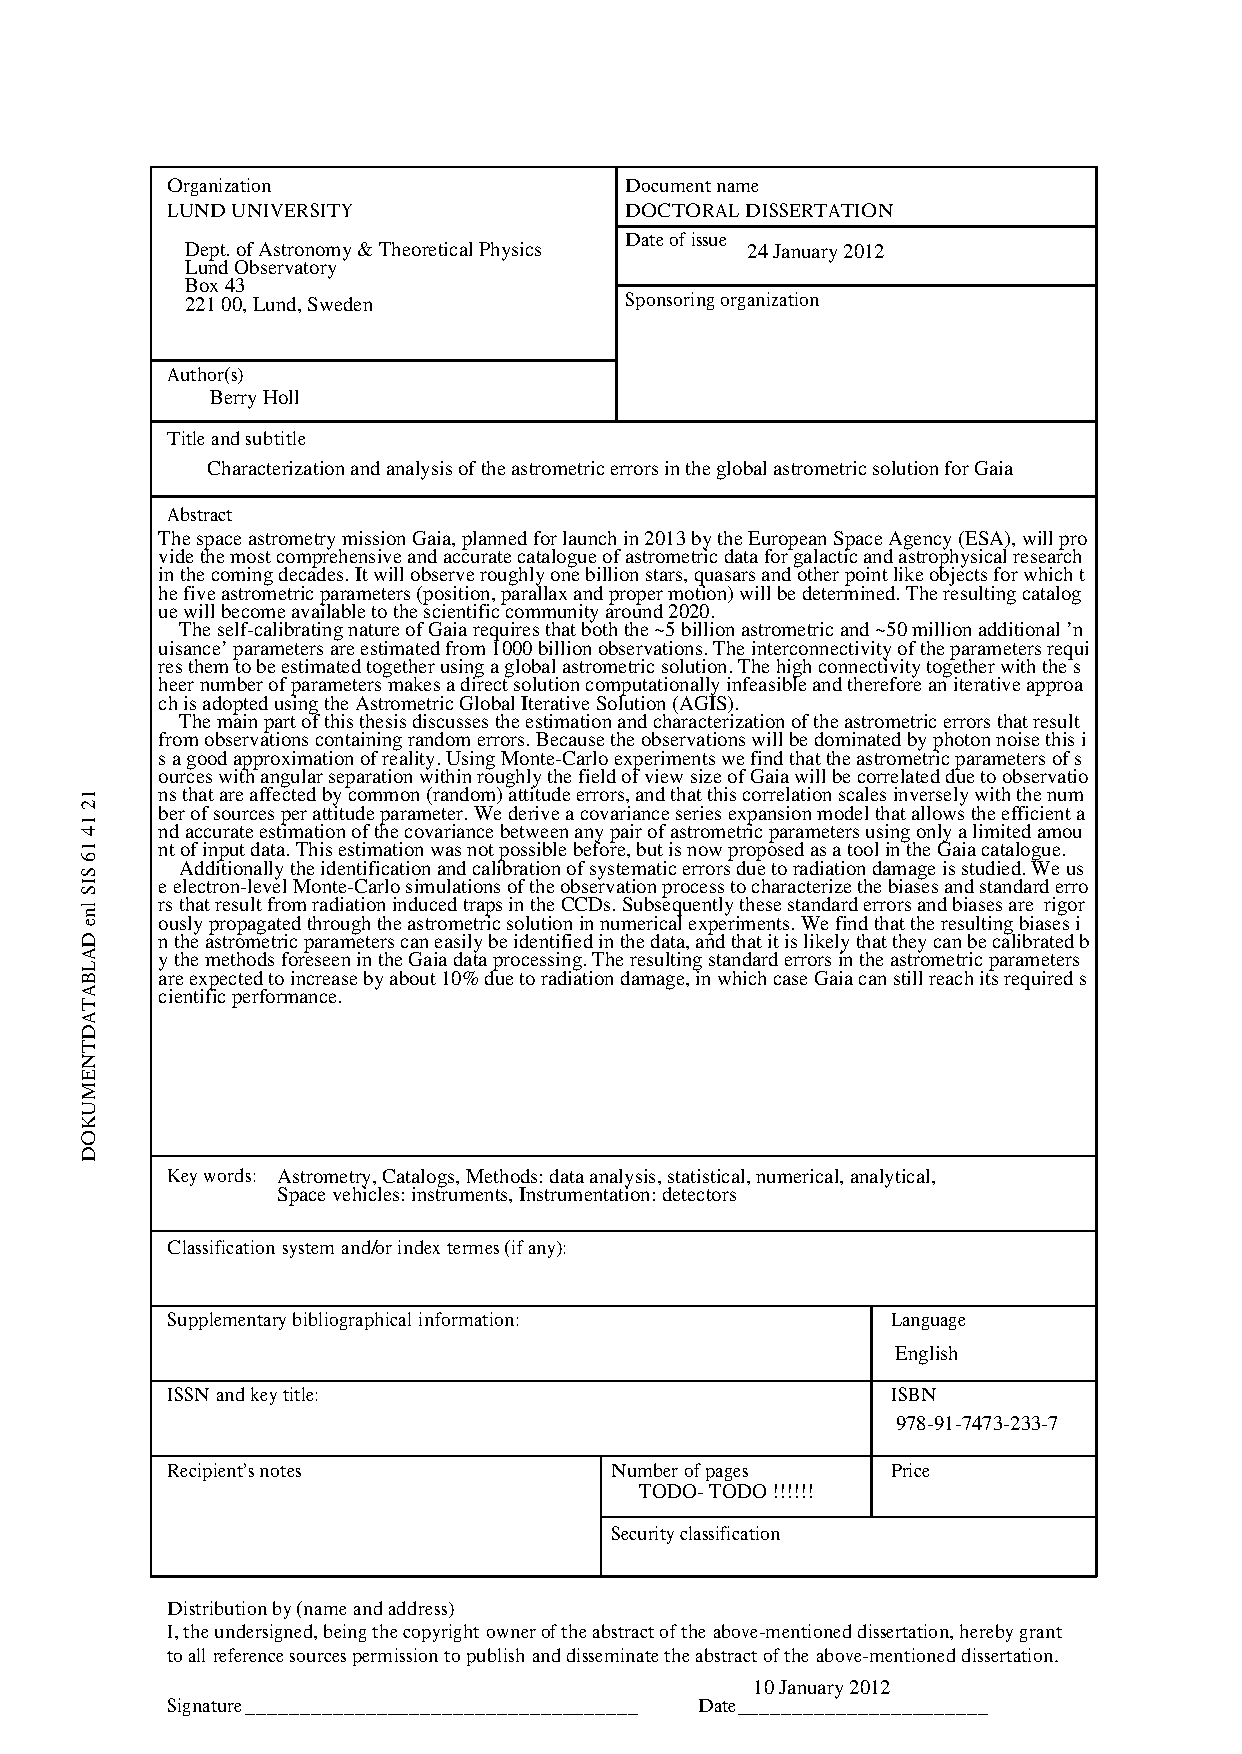
\includepdf[pages=1-1]{datasheetPDF_editable}

%%%%%%%%%%%%%%%%%%%%%%%%%%%%%%%%%%%%%%%%%%%%%%%%%%%%%%%%%%%%%%%%%%%%%%%
% Page five: title and author, without small text. Looks good!

\cleardoublepage
\thispagestyle{empty} % no page number
~
\vfill
\begin{center}
{\HUGE \myMainTitle}
\\[2mm]
{\huge \mySubTitle}

\vfill
{by \myName}

\vfill
% black and white (default):

\includegraphics[width=0.25\textwidth]{LundUniversity_C2line_BLACK.eps}

% Colour text in white so that the spacing is the same as on page three, but with less clutter
\color{white}{
\vspace{10mm}
{\large \myDegree}\\
{\large Thesis advisors: \myAdvisors}\\
{\large Faculty opponent: \myOpponent}\\
\vspace{1cm}
{\footnotesize
\myDefenceAnnouncement
}
}
\\
\end{center}
\vfill


%%%%%%%%%%%%%%%%%%%%%%%%%%%%%%%%%%%%%%%%%%%%%%%%%%%%%%%%%%%%%%%%%%%%%%%
% Page six: Cover image description, ISBN, copyright
\newpage 
\thispagestyle{empty} % no page number
%~
%\vfill
\vspace{-15mm}
A licentiate thesis at a university in Sweden takes either the form of a single,
cohesive research study (monograph) or a summary of research papers
(compilation thesis), which the licentiate student has written alone or together
with one or several other author(s). 

In the latter case the thesis consists of two parts. An introductory text puts
the research work into context and summarizes the main points of the papers.
Then, the research publications themselves are reproduced, together
with a description of the individual contributions of the authors. The
research papers may either have been already published or are manuscripts at
various stages (in press, submitted, or in draft). 

\vfill
{\small
\myCoverFront\\
\\
\myCoverBack\\
\\
\myFundingInformation


\vspace{5mm}
\copyright\, \myName~\myYear\\
\\
\myFaculty, {\myDepartment}
\\
\\
\ISBN: \myISBNprint~(print)\\ % ISBN av svenska ISBN centralen
\ISBN: \myISBNpdf~(pdf)\\ % ISBN av svenska ISBN centralen
%\mySeries\\
\\
Printed in Sweden by Media-Tryck, Lund~University, Lund~\myYear


\includegraphics[width=0.5\textwidth]{miljologotyper}
}


% ===============================================================
% ===================== INSPIRATIONAL QUOTE:  ===================
% ===============================================================
\newpage
\thispagestyle{empty} % No page number on quote page
~
\vspace{140pt}
\begin{flushright}
\textit{Dedicated to\\Humpty -- Dumpty\\bla bla blat}
\end{flushright}


\cleardoublepage


%%%%%%%%%%%%%%%%%%%%%%%%%%%%%%  Table of contents   %%%%%%%%%%%%%%%%%%%%%%%%%%%%%%%%%%%%%%%
\setcounter{page}{1} % Page Roman 1 of the frontmatter
\setcounter{tocdepth}{1}
\setcounter{secnumdepth}{2}
\tableofcontents
% no page number on toc page:
\addtocontents{toc}{\protect\thispagestyle{empty}}


%%%%%%%%%%%%%%%%%%%%%%%%%%%%%%%%% List of publications %%%%%%%%%%%%%%%%%%%%%%%%%%%%%%%%%%%%%%
% Have a long list and want to start on the left page? Here, have a special
% chapter heading for that!
%\addcontentsline{toc}{part}{Part 1: Summary}
%\renewcommand{\chapterheadstartvskip}{}
%{\let\cleardoublepage\relax \let\chapterheadstartvskip\nop 

\newpage
\sect{List of publications\label{sec:paperlist}}
This thesis is based on the following publications, referred to by their Roman numerals:
\vspace{2mm}

{
% Normal font size in this table, afterwards continue with slightly smaller table font size stated in preamble
\floatsetup[table]{font={normalsize},position=top}
\begin{tabularx}{\textwidth}{rX}
% Normal font size in this table, afterwards continue with slightly smaller table font size stated in preamble
\normalsize
\I	  & {\bf \PaperItitle}\\[2mm]
	  & \PaperIauthor\\
          & \PaperIref\\[6mm] 

\II	  & {\bf \PaperIItitle}\\[2mm]
	  & \PaperIIauthor\\
          & \PaperIIref\\[6mm]
\end{tabularx}

All papers are reproduced with permission of their respective publishers.
%Or maybe you need to be more specific? Like: Paper~I and II reproduced with permission \copyright\ ESO\\

% Publications not included in this thesis:
% \vspace{2mm}
%
% \begin{tabularx}{\textwidth}{rX}
% {\sc \phantom{vi}}   & {\bf \PaperNotIncItitle}\\[2mm]
%	  & \PaperNotIncIauthor\\
%          & \PaperNotIncIref\\[5mm] 
%
%\end{tabularx}
%
} % End large font tables, continue with font size stated in preamble


                 
% ===============================================================
% ====================== Acknowledgements:  =====================
\newpage
\sect{Acknowledgements}
\blindtext

% ===============================================================
% ===================== POPULAR SUMMARIES:  =====================

%----------------- SUMMARY IN SWEDISH --------------------
\newpage
\selectlanguage{swedish}
\sect{Populärvetenskaplig sammanfattning på svenska}
\blindtext

% ===============================================================
% ======================= SUMMARY CHAPTER   =====================
% Back to British spelling
\selectlanguage{english}
% Need to add hyphenation corrections? Do like this:
% \hyphenation{as-tro-me-try ana-lysis}

% Page numbers arabic 
\mainmatter
% Reset table counters to not count the publications table
\setcounter{table}{0} 
% Rest page counters, this is where it all starts!
\setcounter{page}{1}

\chap{\myTitle}
% Fancy a quote?
\newpage

%%%%%%%%%%%%%%%%%%%%%%%%%%%%%%%%%%%%%%%%% Actual kappa %%%%%%%%%%%%%%%%%%%%%%%%%%%%%%%%%%%%%%%%%
\part{Research motivation}
\chapter{Introduction to quantum chromodynamics}
\def \imgpath {"./figures/intro"}

This chapter serves as an introduction to particle physics, QCD, and phenomenology of high energy QCD interactions, with the focus on multiple partonic interactions and string formations. Furthermore, it introduces the physics of QCD matter and the deconfinement of hadrons.

\section{Standard Model of elementary particles}

The Standard Model (SM) of particle physics is a set of theories describes \textit{elementary} constituents of matter and their interactions via fundamental forces of the Universe. It has been formulated in the 1970s, combining frameworks of quantum field theory (QFT), gauge symmetries, and spontaneous symmetry breaking.

Matter particles in the SM are classified into two main categories: quarks and leptons. Quarks come in six flavours (\textit{up, down, charm, strange, top, and bottom}) and form hadrons, i.e.\ \textit{baryons} ($qqq$) and \textit{mesons} ($q\bar{q}$). The lepton sector also comprises six flavours (\textit{electron, muon, tau, and their corresponding neutrinos}). Quarks and leptons are fermions with an intrinsic spin $1/2$. Furthermore, matter particles in the SM also come with associated antiparticles, which have opposite quantum numbers but the same mass.

The interactions between matter particles in the SM are mediated by an exchange of gauge bosons. There are three fundamental forces in the SM, described by four types of vector bosons (ordered by their typical strength): 
\begin{enumerate}
\item \textit{Strong force}, mediated by the gluon.
\item \textit{Electromagnetic force}, mediated by the photon.
\item \textit{Weak force}, mediated by the massive bosons $W^\pm$ and $Z^0$.
\end{enumerate} 

Moreover, the interactions are associated with local gauge symmetries, which determine their mathematical structure. The symmetry group for the SM is SU($3$)$\times$SU($2$)$\times$U($1$), corresponding to the strong and the electroweak sector. \cite{tanabashiReviewParticlePhysics2018}

In addition, the SM also includes the scalar Higgs boson, which is responsible for giving mass to other elementary particles. This is achieved via the Higgs mechanism \cite{higgsBrokenSymmetriesMasses1964, englertBrokenSymmetryMass1964}, which involves the spontaneous breaking of the electroweak symmetry in the early universe. The Higgs boson was discovered experimentally at the Large Hadron Collider (LHC) in 2012 by the ATLAS \cite{theatlascollaborationObservationNewParticle2012} and CMS \cite{thecmscollaborationObservationNewBoson2012} collaborations, confirming a key prediction of the SM.

Nevertheless, the SM has several limitations, including its inability to account for dark matter, explain why the particle masses span over several orders of magnitude, and the CP violation problem related to the observed matter-antimatter asymmetry in the Universe. These are actively investigated in Beyond Standard Model (BSM) theories.

\begin{figure}[H]
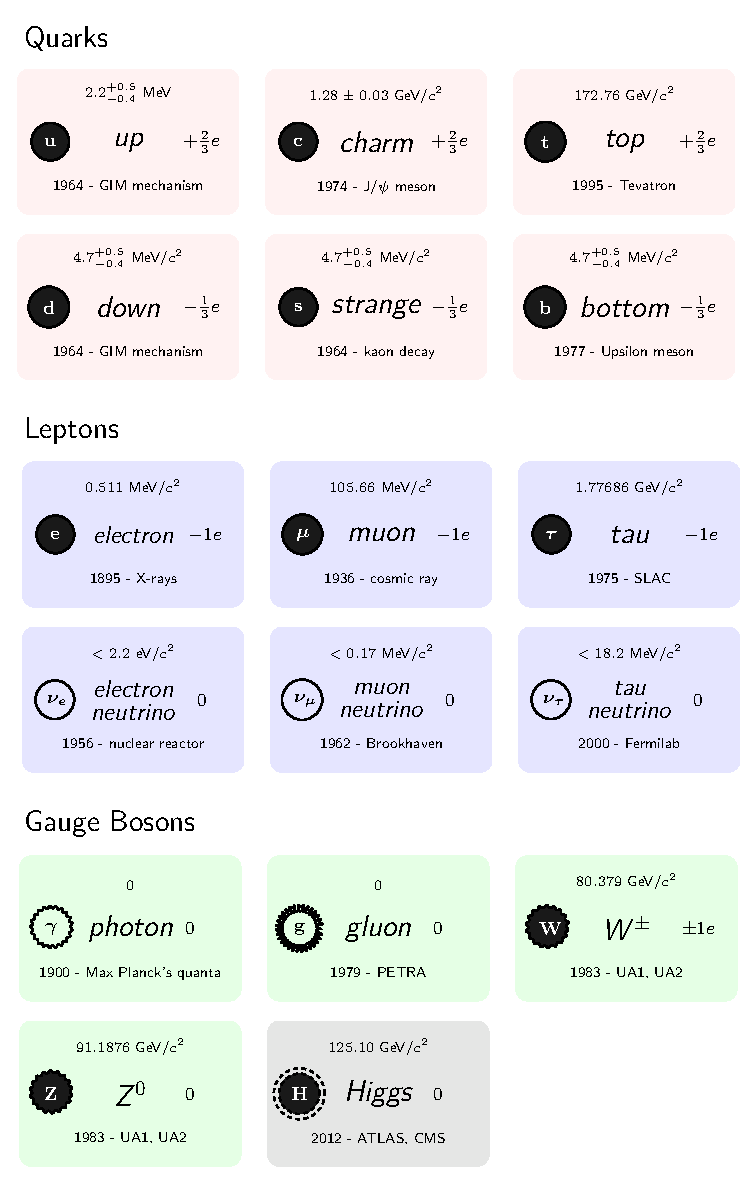
\includegraphics[width=0.90\textwidth]{\imgpath/SM.pdf}
\caption{Particle of the Standard Model, listed together with their mass, electric charge, and the  year and means of discovery (going clockwise from the top). VALUES NEED TO BE FIXED.}
\end{figure}

\section{Coordinate systems and kinematic observables}

Particles in HEP processes are described by their Lorentz-invariant four-vectors, $\bm{x} = (ct, x, y, z)$ and $\bm{p} = (E/c, p_x, p_y, p_z) = (E/c, \vec{\pt} , p_z)$, where $|\vec{\pt}| \equiv \sqrt{p_x^2+p_y^2}$. In LHC experiments, the coordinate system is defined such that the $x$-axis points in the direction of the centre of the LHC, and the $z$-axis points in the direction of the beam, as shown in Fig.~\ref{fig:intro:coordinates}. In addition to the standard Cartesian coordinates, two observables, $\varphi$ (azimuthal angle) and $\eta$ (pseudorapidity), are used to describe the position and momentum of particles relative to the interaction point, which is located at $x = y = z = 0$. Pseudorapidity is defined as a function of the polar angle $\theta$, where 
\begin{align}
\eta = -\ln(\tan(\theta/2)) \quad .
\end{align}
For high-momentum particles ($E \simeq pc$), pseudorapidity is an approximation of the rapidity relative to the beam, given by 
\begin{align}
y = \frac{1}{2} \ln \frac{E + p_z c}{E - p_z c} \quad .
\end{align}
Rapidity is a convenient quantity to use because it transforms additively under Lorentz boosts, unlike velocity. In these coordinates, the following relations hold:
\begin{align}
p_x = |\vec{\pt}| \cos \varphi \, , \quad \
p_y = |\vec{\pt}| \sin \varphi \, , \quad \
p_z = |\vec{p} \,| \sinh \eta \, .
\end{align}

\begin{figure}[H]
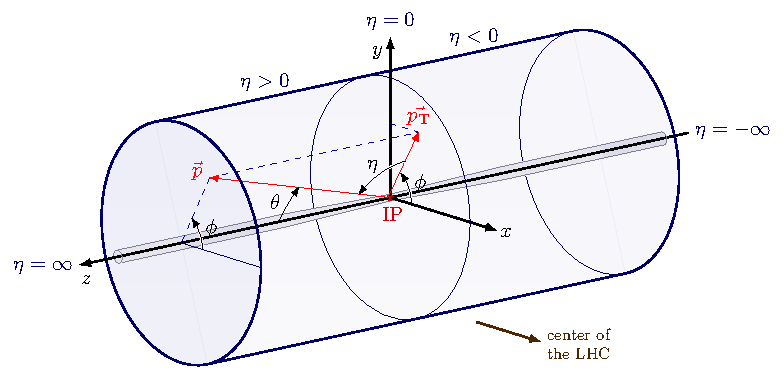
\includegraphics[width=0.85\textwidth]{\imgpath/coordinates.pdf}
\caption{Coordinate system of an LHC experiment, with the interaction point in the centre.}
\label{fig:intro:coordinates}
\end{figure}

\section{Quantum electrodynamics, electrons, and photons}

In many aspects, QCD is a very similar theory to the simpler and better explored theory QED. In QFT, dynamics of particles can be provided in terms of its Lagrangian density $\mathcal{L}$, from which equations of motions can be derived and which is also used to calculate interaction probabilites. The QED theory with a local U($1$) symmetry has its $\mathcal{L}_\mathrm{QED}$ defined as:

\begin{equation}
\mathcal{L}_\mathrm{QED} = \bar{\psi}(i \slashed \partial - m)\psi - \frac{1}{4}F_{\mu\nu}F^{\mu\nu} - e\bar{\psi}\slashed A \psi \quad ,
\end{equation}
where $\psi$ is the electron field with mass $m$ and electric charge $e$, $F_{\mu\nu}$ the electromagnetic field-strength tensor, and Feynman slash notation is employed. The first part describes the dynamics of the electron fields, the second part describes the dynamics of the electromagnetic field, and the last part describes the interaction of electrons and photons with a coupling strength $e$. Using Feynman diagrams, they can be visualised as:
\begin{figure}[H]
\adjustbox{valign=m}{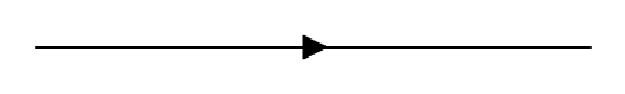
\includegraphics[width=0.19\textwidth]{\imgpath/qed1.pdf}}\hspace{1em}
\adjustbox{valign=m}{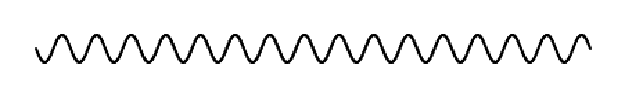
\includegraphics[width=0.19\textwidth]{\imgpath/qed2.pdf}}\hspace{1em}
\adjustbox{valign=m}{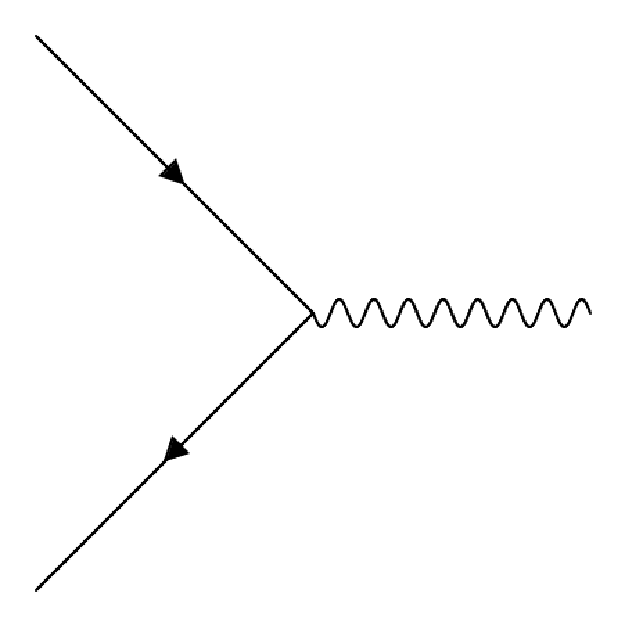
\includegraphics[width=0.19\textwidth]{\imgpath/qed3.pdf}}
\end{figure}

In QED interactions, each vertex depicted in the Feynman diagrams contributes to the probability of the process with a coefficient $\alpha$ (to the matrix elements as $\sqrt{\alpha}$, which is the coupling constant defined as $\alpha = e^2/4\pi$. This constant is generally small, which allows for interactions to be calculated using perturbation theory as an expansion series in $\alpha$. The contributions to the series correspond to different Feynman diagrams representing the possible interaction processes, and they are ordered in powers of $\alpha$ based on the complexity of the diagrams.

Contributions from higher orders, such as the electron loop depicted below, lead to ``screening" of the effective charge at large distances/small momenta, which makes the coupling constant dependent on the scale of the process $\mu$. For example, at low energies corresponding to atomic scales, $\alpha \approx 1/137$, but at scales of the $Z^0$ boson mass, $\alpha \approx 1/127$ \cite{fritzschFundamentalConstantsHigh2002}. The \textit{running} of this coupling is given by the $\beta$ function, $\beta(\alpha) \equiv \frac{\partial \alpha}{\partial \log \mu^2}$, and it can be calculated by quantifying the effective coupling strengths at various orders of perturbation theory and using renormalisation group tools \cite{delamotteHintRenormalization2004}, although renormalisation is a more general concept. In QED, the screening leads to a positive sign in $\beta$ calculated at lowest order, which means that when solving for $\alpha$ by integrating, $\alpha$ grows with energy scale\footnote{The scale at which QED eventually breaks down due to this increase is well above the Plack mass.}.

\begin{figure}[H]
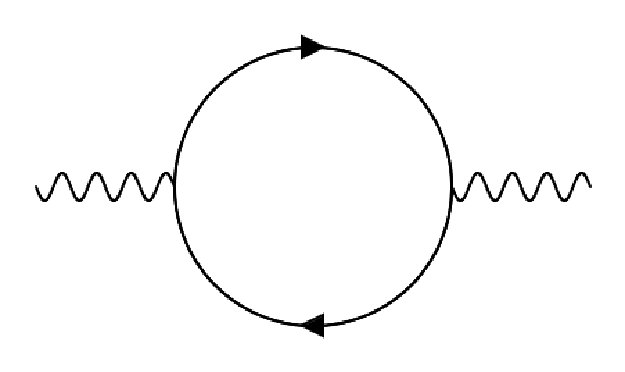
\includegraphics[width=.26\textwidth]{\imgpath/qedloop.pdf}
\end{figure}

Renormalisation is also used when calculating physical quantities where loop contributions lead to divergences, which are then absorbed into the parameters of the theory. The success of these procedures and the QED theory as a whole is validated by excellent prediction power for experimental measurements, such as the magnetic moment of an electron \cite{odomNewMeasurementElectron2006}.

\section{Quantum chromodynamics, quarks, and gluons}

In QCD, particles have an additional quantum number called colour charge: red, green, and blue. Thus, there are three quarks of each flavour and eight gluons mediating interactions between. Gluons also carry colour charges, which allows them to interact with each other, making the theory non-Abelian. The QCD Lagrangian is symmetric under local SU($3$) transformations and takes the shape of:

\begin{align}\label{eq:intro:lqcd}
\mathcal{L}_\mathrm{QCD} &= \sum_{f}^{n_f} \bar{\psi}_i^{(f)}(i \slashed D_{ij}-m_f \delta_{ij} ) \psi_j^{(f)} \, - \frac{1}{4} \sum_a^8 F^{\mu\nu}_a F_{\mu\nu}^a \quad , \\
D^\mu_{ij} &\equiv \partial^\mu \delta_{ij} + i g_s t^a_{ij}A^\mu_a \quad , \\
F^a_{\mu\nu} &\equiv \partial_\mu A^a_\nu - \partial_\nu A^a_\mu - g_s f_{abc} A^b_\mu A^c_\nu \quad ,
\end{align}
where $\psi$ are the quark fields of $n_f$ different flavours with mass $m_f$ and colour $i,j$, $D^\mu_{ij}$ the covariant derivative with the coupling strength $g_s$ and eight SU($3$) generators given by matrices $t^a_{ij}$, and $A_a^{\mu}$ are the gluon fields \cite{altarelliQCDPrimer2002}. Lastly, $F^a_{\mu\nu}$ is the field-strength tensor with $f_{abc}$ being structure constants. The Lagrangian now also contains terms with interactions between gluons. In the representation of Feynman diagrams, for the interactions, there is:
\begin{figure}[H]
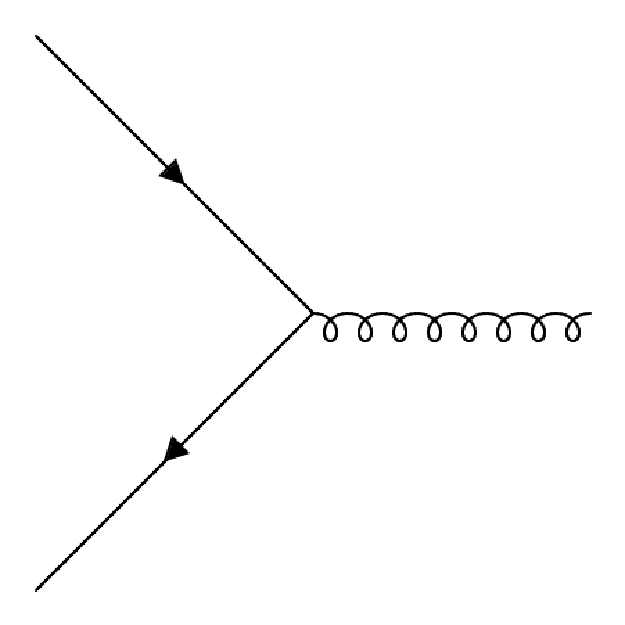
\includegraphics[width=0.19\textwidth]{\imgpath/qcd3.pdf}\hspace{1em}
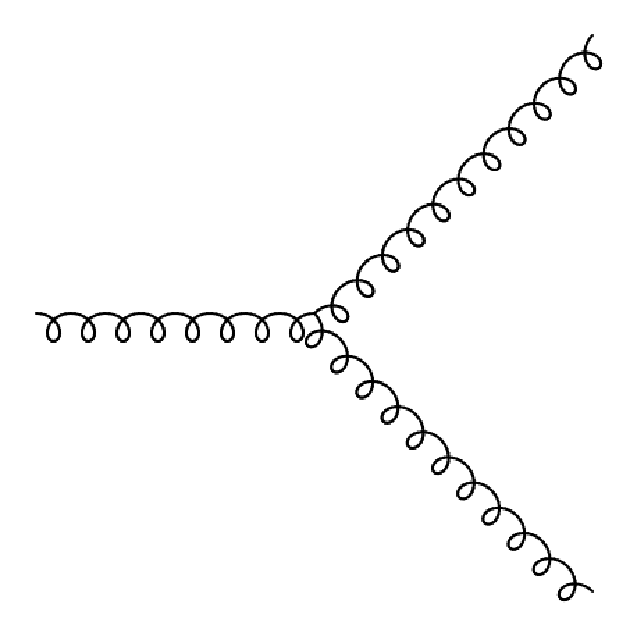
\includegraphics[width=0.19\textwidth]{\imgpath/qcd4.pdf}\hspace{1em}
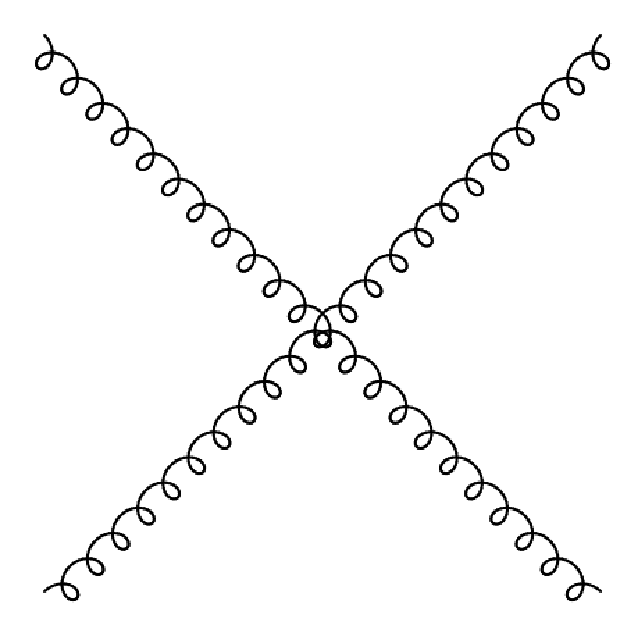
\includegraphics[width=0.19\textwidth]{\imgpath/qcd5.pdf}
\end{figure}

Similarly to the QED case, the strong coupling constant can be defined as $\alpha_s = g^2/4\pi$. However, when considering its modifications due to virtual corrections, in addition to the quark loop, there is also a gluon loop.:
\begin{figure}[H]
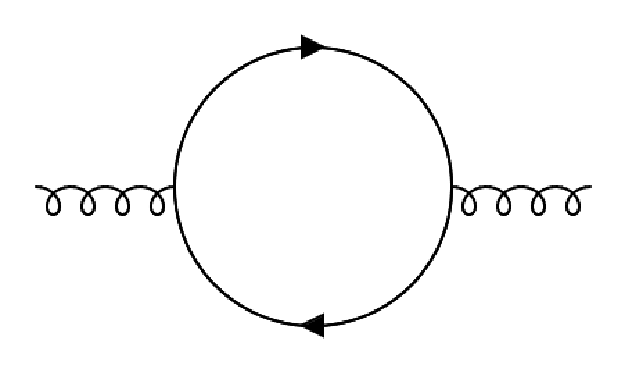
\includegraphics[width=0.26\textwidth]{\imgpath/qcdloop1.pdf}\hspace{2em}
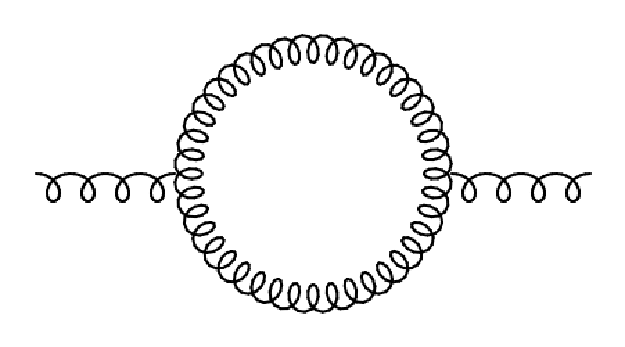
\includegraphics[width=0.26\textwidth]{\imgpath/qcdloop2.pdf}
\end{figure}

The gluon loop contributes to the $\beta$ function in an opposite and larger way than the quark loop, and so overall, there is an \textit{anti-screening} effect instead and a negative sign in the calculated one-loop $\beta$ function. The running of the coupling can be calculated as:
\begin{align}
\alpha_s (\mu) = \frac{1}{b_0 \log ( \mu^2 / \Lambda_\mathrm{QCD}^2 )} \quad ,
\end{align} 
where $b_0$ is a constant computed from the loop calculations, $b_0 = \frac{11-\frac{2}{3}n_f}{4\pi}$ \cite{politzerReliablePerturbativeResults1973}. The introduced $\Lambda_\mathrm{QCD}$ is a scale parameter of the theory corresponding to the energy where the coupling becomes infinite, and depends on the definition of $\alpha_s$ and the number of available quark flavours $n_f$ \cite{altarelliQCDPrimer2002}. It ranges between $200$ and $\mevcc{300}$ \cite{deurQCDRunningCoupling2016}.

From the running, it is evident that the coupling strength decreases with increasing energy, which is known as \textit{asymptotic freedom} \cite{politzerReliablePerturbativeResults1973,grossAsymptoticallyFreeGauge1973} and corresponds to the fact that strong interaction is short-ranged. On the other hand, at low values, $\alpha_s$ diverges, which is related to the fact that quarks are bound to hadrons -- \textit{quark confinement}. The evolution of $\alpha_s$ also limits the applicability of perturbation theory at low energy regimes; calculations from perturbative QCD (pQCD) are relevant at leading orders starting typically from $1-\gevcc{2}$. The measured $\alpha_s(\mu)$ is shown in Fig.~\ref{fig:intro:alpha}, and at scales of the $Z^0$ boson mass is approximately $0.1185 \pm 0.0006$ \cite{dissertoriDeterminationStrongCoupling2016, particledatagroupReviewParticlePhysics2022}.

\begin{figure}[H]
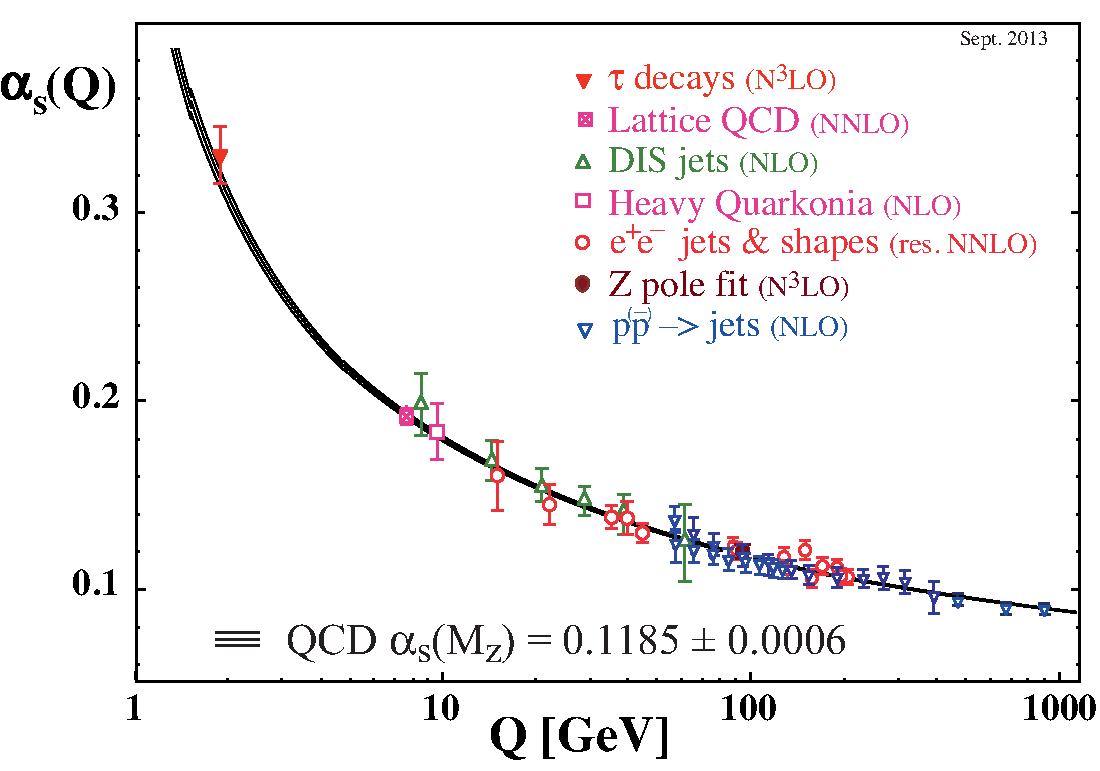
\includegraphics[width=0.55\textwidth]{\imgpath/alpha.pdf}
\caption{Strong coupling constant determined at different energy scales through various measurements and numerical calculations (data points) and compared with theoretical predictions from QCD. \cite{dissertoriDeterminationStrongCoupling2016}}
\label{fig:intro:alpha}
\end{figure}

\section{From partons to hadrons}

\subsection{Initial and Final State Radiation}

In QFT, charged particles are surrounded by a cloud of virtual particles, which can be thought of as fluctuations in the particle's field. For example, the electron state can be described as a superposition of the bare electron plus additional massless bosons:
\begin{align}
|\mathrm{e}\rangle_\mathrm{phys} = |\mathrm{e}\rangle + |\mathrm{e}\gamma\rangle + |\mathrm{e}\gamma\gamma\rangle + \ldots
\end{align}
and, at higher orders, pairs of virtual electrons. The fluctuations continuously form and recombine, with their lifetime depending on their energy and momentum. Specifically, the lifetime of a fluctuation with energy $\omega$ and transverse momentum $k_\mathrm{T}$ can be approximated as:
\begin{align}
\tau \approx \frac{\omega}{k_\mathrm{T}} \quad .
\end{align}
This implies that fluctuations with smaller-$k_\mathrm{T}$ live longer. \cite{prestelParticlePhysicsPhenomenology}

As illustrated in Fig.~\ref{fig:intro:isrfsrsketch}, the coherent mixed state of the bare charge and the field fluctuations can be disturbed by the presence of an interaction. Intuitively, this interaction can change the energy and momentum of the fluctuations, their formation and recombination, and lead to the emission of radiation in two ways:
\begin{enumerate}
\item a fluctuation is kicked on-shell by the interaction and part of the field continues in its original direction, which leads to Initial State Radiation (ISR);
\item as a result of the field of the scattered particle rearranging itself , which can be a source of Final State Radiation (FSR).
\end{enumerate}

In both of the cases, a larger momentum transfer implies more radiation. \textit{For hard, wide angle emissions, cross sections can be calculated perturbatively at fixed orders}. 

Soft and collinear emissions, however, lead to infra-red divergences ($\propto \frac{1}{\omega}$,$\propto \frac{1}{k_\mathrm{T}^2}$) and thus, need to be factorised away from the amplitudes or the cross sections and then described using resummation techniques. Without any emissions, the probabilities of finding electrons and photons of fractional momentum $x$ with respect to the whole system are:
\begin{align}
f_\mathrm{e} (x) = \delta (1-x) \, , \quad \ f_\gamma(x) = 0 \, ,
\end{align}
When considering the emissions above some scales parametrised by the resolution parameter $Q^2$, these probabilities, however, evolve according to the DGLAP equation \cite{altarelliAsymptoticFreedomParton1977} :
\begin{align}
\label{eq:intro:dglap}
\frac{\partial}{\partial\ln Q^2}
\begin{pmatrix}
f_e(x, Q^2)\\
f_{\gamma}(x, Q^2)
\end{pmatrix}
&= \frac{\alpha_\mathrm{em}}{2\pi}
\int_x^1 \frac{dz}{z}
\begin{pmatrix}
P_{ee}(z) & P_{e\gamma}(z)\\
P_{\gamma e}(z) & P_{\gamma\gamma}(z)
\end{pmatrix}
\begin{pmatrix}
f_e\left(\frac{x}{z}, Q^2\right)\\
f_{\gamma}\left(\frac{x}{z}, Q^2\right)
\end{pmatrix} \quad ,
\end{align}
where $P_{ij}(z)$ are the splitting probability functions of a particle $i$ emitting a particle $j$.

In QCD, the behaviour is analogous, with $\alpha_\mathrm{em} \rightarrow \alpha_s$, $e\rightarrow q$, and $\gamma \rightarrow g$. \cite{prestelParticlePhysicsPhenomenology}

\begin{figure}[H]
\subfloat[][]{\adjustbox{valign=m}{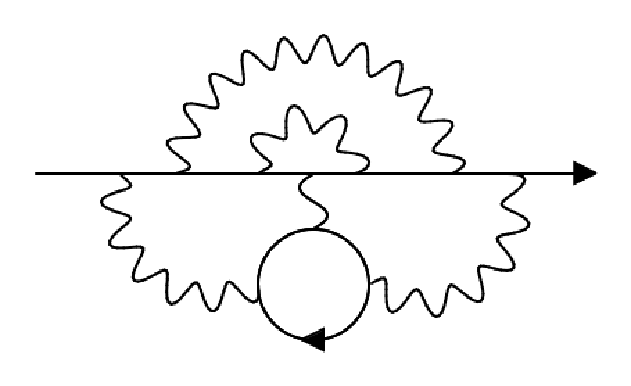
\includegraphics[width=.240\textwidth]{\imgpath/eisr1.pdf}}\adjustbox{valign=m}{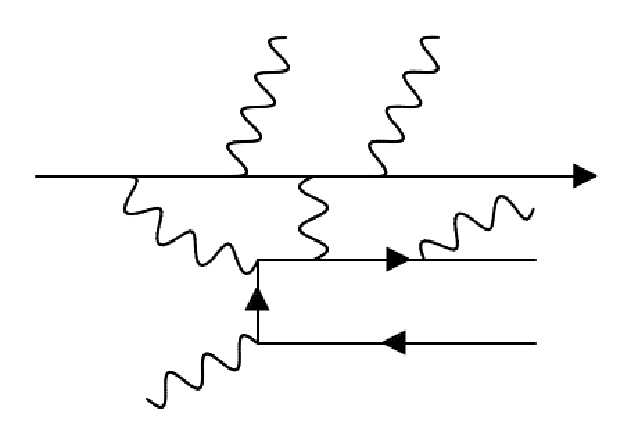
\includegraphics[width=.240\textwidth]{\imgpath/eisr22.pdf}}}
\subfloat[][]{\adjustbox{valign=m}{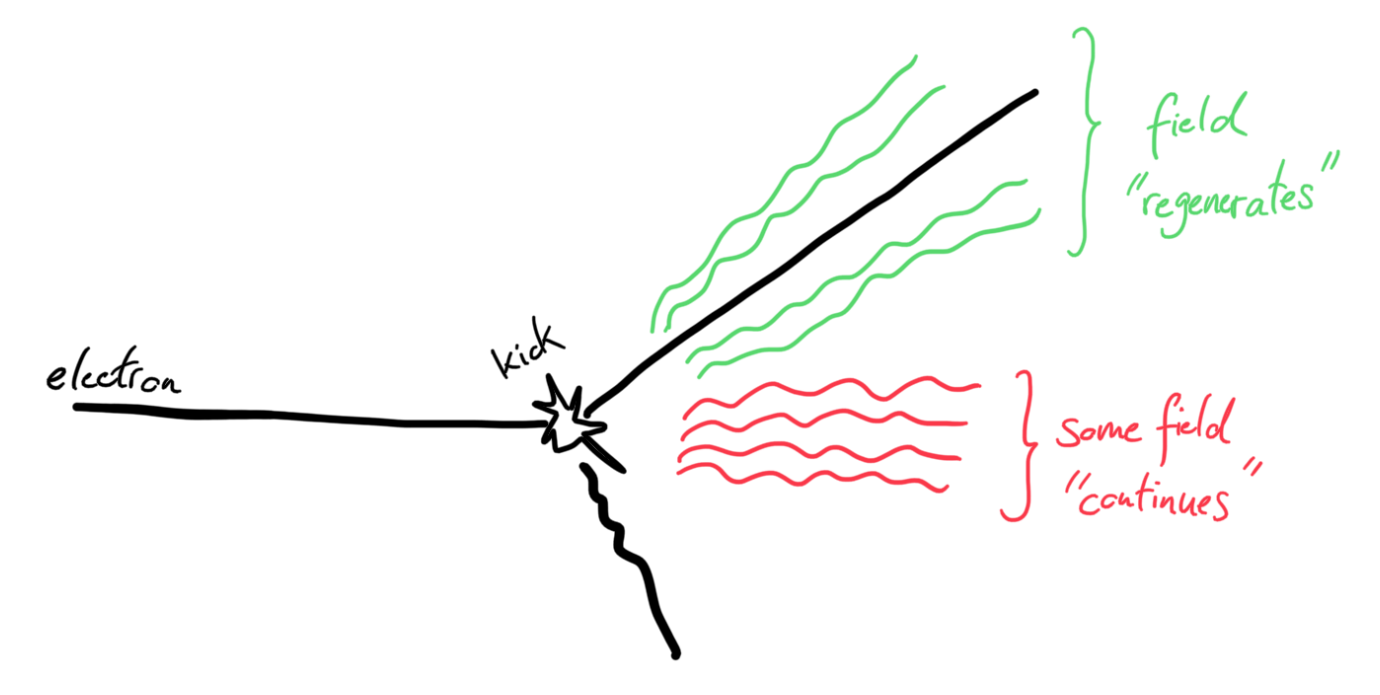
\includegraphics[width=.480\textwidth]{\imgpath/isrfsr2.png}}}
\caption{\textbf{(a)} Illustration of the field fluctuations before and after the state coherence gets disturbed by an external actor. \textbf{(b)} Illustration of emmisions of radiation in a scattering process.}
\label{fig:intro:isrfsrsketch}
\end{figure}

\subsection{Factorisation theorem}

The evolution equation (\ref{eq:intro:dglap}) implies that the probabilities of observing emissions with a fractional momentum $x$ depend on the resolution $Q^2$. In QCD, 
\begin{enumerate}
\item when applied to the initial state, they are known as parton distribution functions (PDFs) and determine the probabilities of finding partons\footnote{Partons refer to the valence quarks, sea quarks, and gluons inside hadrons.} in the composite hadronic state. 
\item When applied to the final state, they are called fragmentation functions, and determine the probabilities of measuring fragments of the outgoing particles.
\end{enumerate}

This leads to the factorisation theorem \cite{collinsFactorizationHardProcesses2004} for processes involving collisions of two hadrons, which separates the perturbatively calculable partonic cross section from the non-perturbative partonic evolution and hadronisation. The theorem can be expressed as follows:
\begin{align}\label{eq:intro:facto}
\sigma = f_i^A(x_i,\mu_F)f_j^B(x_j,\mu_F) \otimes \hat{\sigma}_{ij\to n}(\mu_F,\mu_R) \otimes D_{n \to n'} \, .
\end{align}
Here, $i$ and $j$ are the initial partons, $\hat{\sigma}_{ij\to n}$ is the partonic cross section, $D_{n \to n'}$ is the process-specific fragmentation function for evolving the partons $n$ into the particles' final state $n'$, and $\mu_F$ and $\mu_R$ are the factorisation and renormalisation scales, respectively. The factorisation scale, $\mu_F$, determines the scale below which the emissions are absorbed into the PDFs. The theorem is depicted in Fig.~\ref{fig:intro:factorisation}.

\begin{figure}[H]
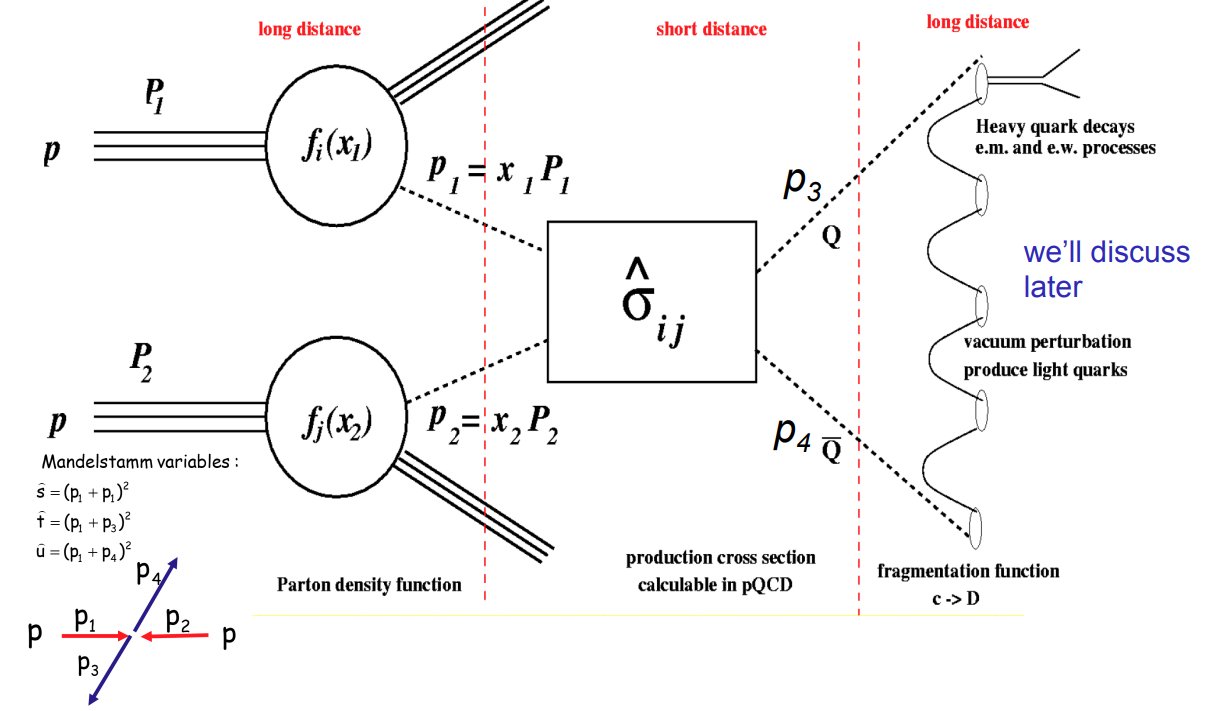
\includegraphics[width=0.65\textwidth]{\imgpath/factorisation.png}
\caption{Illustration of the factorisation theorem. (NEEDS TO BE REMADE).}
\label{fig:intro:factorisation}
\end{figure}

\subsection{Parton distribution functions}

The PDFs defining the probabilities of finding quarks and gluons in nucleons can be determined experimentally at hadron-electron colliders such as HERA \cite{cooper-sarkarExtractionProtonParton2008}. They are determined from measurements of deep inelastic scatterings in a range of energies and momentum transfers. They are displayed in Fig.~\ref{fig:intro:pdfs} as a function of the fractional momentum $x$ (also called Bj\"orken $x$). 

According to collider kinematics, $x \propto \frac{1}{\sqrt{s}e^y}$, therefore, the partonic composition of ultra-relativistic hadrons is dominated by gluons. Following unitarity principles and BK evolution equation \cite{marquetBalitskyKovchegovEquationFull2005}, it is expected that gluons start recombining and the gluonic content saturates as $x\rightarrow0$. This is actively reseached \cite{starcollaborationEvidenceNonlinearGluon2022}, however, not directly measured yet. Additionally, it should be noted that in ultra-relativistic heavy nuclei, the partons are modified in the contracted nuclear environment and the PDFs are referred to as nPDFs.

\begin{figure}[H]
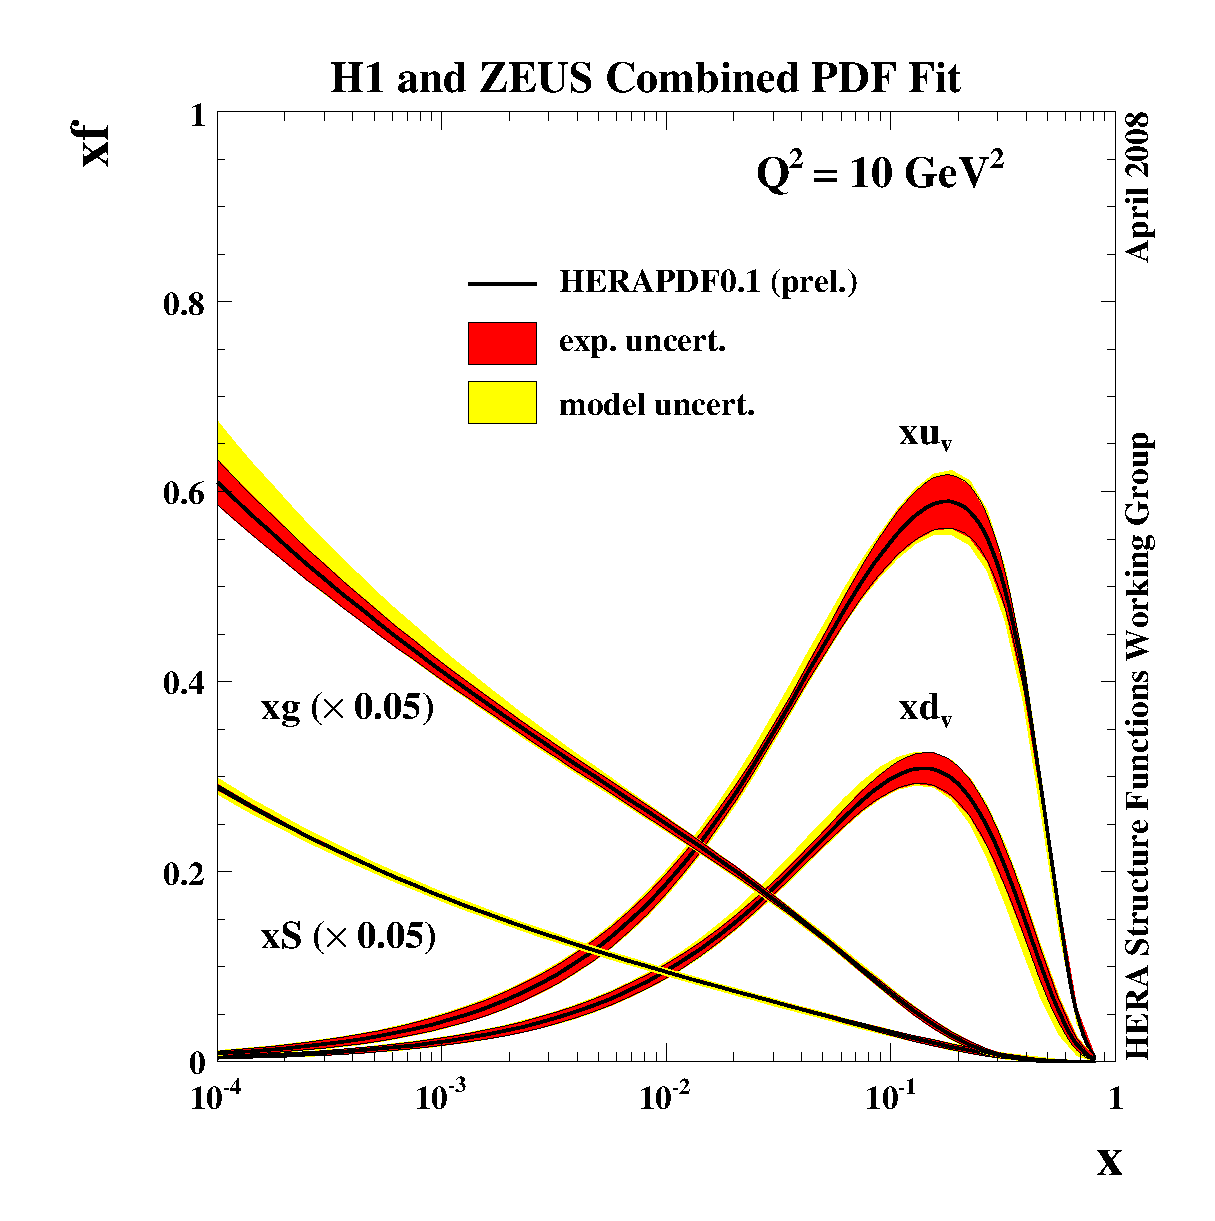
\includegraphics[width=0.4\textwidth]{\imgpath/pdf.eps}
\caption{Parton distribution functions determined in ep scatterings at HERA as a function of the fractional momentum for the up, down, sea quarks, and gluons. \cite{cooper-sarkarExtractionProtonParton2008}}
\label{fig:intro:pdfs}
\end{figure}

\subsection{Parton fragmentation and the Lund string}

After the scattering process, the produced partons continue to fragment by emitting more partons in a process called the parton shower. Since the coupling strength in QCD increases with decreasing the energy scale of the splitting, this leads to the production of many soft, collimated emissions known as jets. The partonic evolution continues until the virtuality of the partons reaches the hadronization scale ($\approx \Lambda_\mathrm{QCD}$). There are multiple frameworks within QCD to describe the evolution of partons into their final state, such as using the DGLAP equations or the so-called dipole formalism.

Once the partonic final state is reached, the partons hadronise into the observable mesons and baryons. The hadronisation process is not calculable in QCD and requires phenomenological models to describe it. One such model is the Lund string model \cite{ferreres-soleSpaceTimeStructureHadronization2018}, which describes hadronisation as the breaking of a color string between the quarks in the final state. In this model, the energy stored in the color string is converted into the mass of new hadrons.

According to confinement, hadronisation should involve at least two partons with complementary colours. In QCD, the $q\bar{q}$ potential takes the shape of
\begin{align}\label{eq:intro:qqpot}
V_{q\bar{q}} \approx - \frac{4}{3}\frac{\alpha_s \hbar c}{r} + \kappa r \quad ,
\end{align}
where $\kappa$ is a parameter with value around $1 \mathrm{GeV} /\mathrm{fm}$. In the non-perturbative regime (long distances), the potential is dominated by the linear part, which is reminiscent of a system bound by a string with tension $\kappa$. This is taken advantage of by the Lund string model -- a $q$ and $\bar{q}$ pair separated by distance $\Delta x$ is bound by a color field (string) with energy $\kappa \Delta x$. 

If the $q$ and $\bar{q}$ continue separating as a result of the scattering, the energy stored in the color field increases. At some point, it can become energetically favourable to produce a new $q\bar{q}$ pair out of vacuum, which is a quantum mechanics tunnelling phenomenon characterised by the probability:
\begin{align}
\frac{\mathrm{d}P}{\mathrm{d}m_\mathrm{T}} \propto \exp \left( -\frac{\pi m_\mathrm{T}^2}{\kappa} \right) \quad ,
\label{eq:intro:tunnel}
\end{align}
where $m_\mathrm{T}$ is the transverse mass of the produced quarks. Otherwise, the $q\bar{q}$ system starts contracting and oscillates with a period $T = 2 E_\mathrm{kin}/\kappa$, where $E_\mathrm{kin}$ is its maximum kinetic energy. The produced $q$ and $\bar{q}$ then connect by new color fields to the original pair. This process repeats itself resulting in a cascade of many $q\bar{q}$ pairs connected by many color strings. In this description, baryons can also be created by double tunnelling of a $qq\overline{qq}$ pair. The process is illustrated in Fig.~\ref{fig:intro:lundstring}.

\begin{figure}[H]
\subfloat[][]{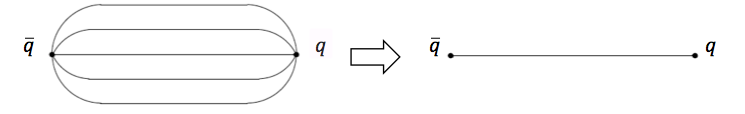
\includegraphics[width=.330\textwidth]{\imgpath/tubelike.png}}
\subfloat[][]{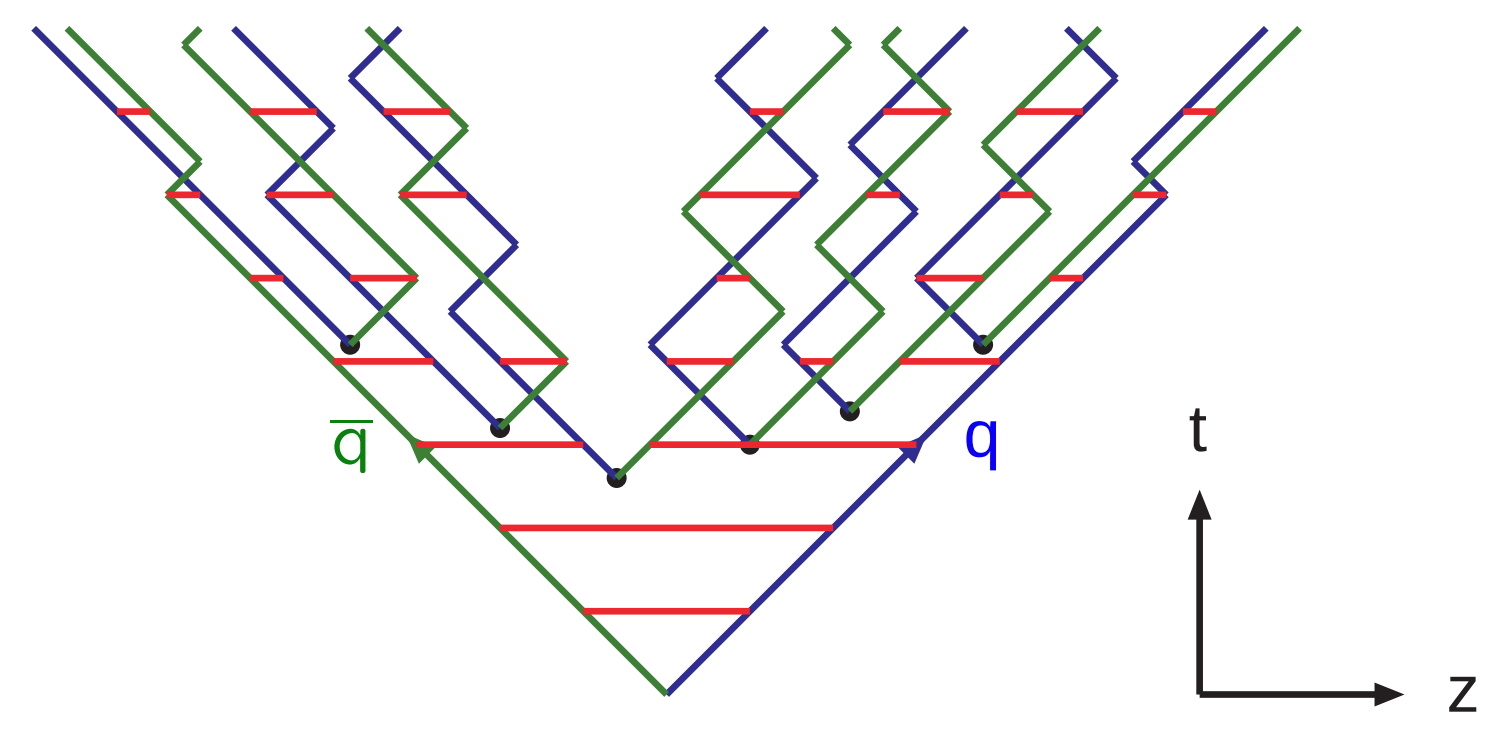
\includegraphics[width=.330\textwidth]{\imgpath/lundstring.png}}
\subfloat[][]{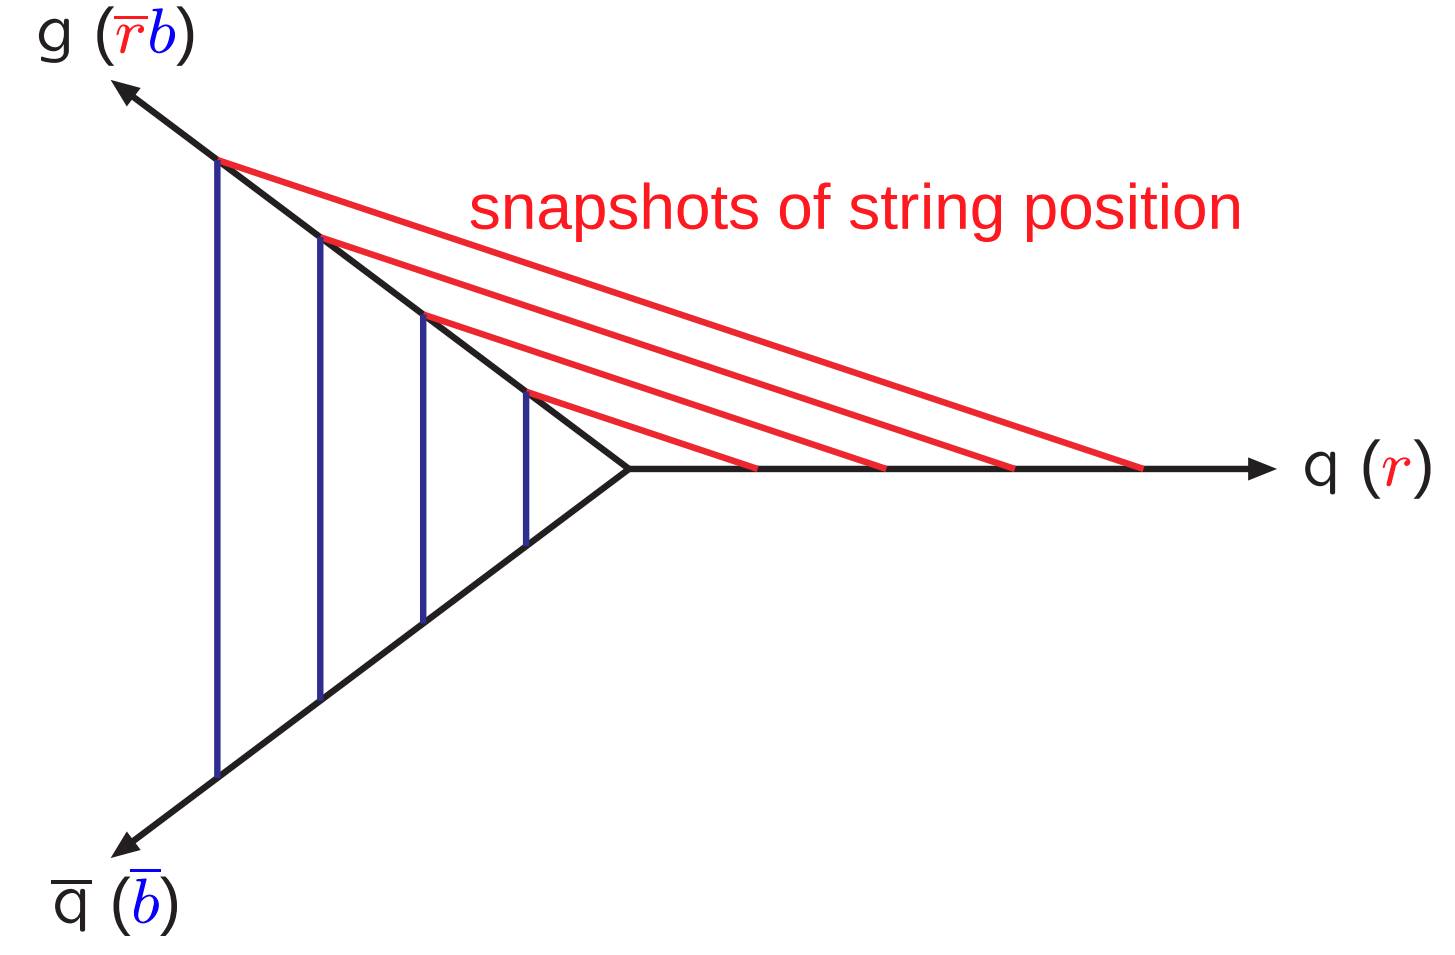
\includegraphics[width=.330\textwidth]{\imgpath/lundgluon.png}}
\caption{\textbf{(a)} Illustration of the color field between two quarks and its simplified representation with a string  \cite{ferreres-soleSpaceTimeStructureHadronization2018}. \textbf{(b)} Illustration of the string splitting by producing new $q\bar{q}$ in the $t-z$ plane \cite{ferreres-soleSpaceTimeStructureHadronization2018}. \textbf{(c)} Visualisation of the treatment of gluons in the Lund string model \cite{sjostrandQCDBSMPYTHIA2011}.}
\label{fig:intro:lundstring}
\end{figure}

Equation \ref{eq:intro:tunnel} also implies that production of strange quarks is suppressed by a factor of 
\begin{align}\label{eq:intro:rho}
\rho = \exp \left( -\frac{\pi (m^2_s - m^2_{u,d})}{\kappa} \right) \quad .
\end{align}
This parameter is typically tuned to data, as substituting constituent ($m_s \approx \gevcc{0.5}$, $m_{u,d} \approx \gevcc{0.33}$) versus current masses ($m_s \approx \gevcc{0.1}$, $m_{u,d} \approx 0$) leads to considerable differences underestimating and overestimating data, respectively.

For a $q\bar{q}g$ system, in this model, the gluon connects to the quark and antiquark and is effectively treated as a ``kink" on the color field, adding energy and momentum to the $q\bar{q}$ string (stretching it in its direction), as visualised in Fig.~\ref{fig:intro:lundstring}.

It should be noted that in the paradigm of AA collisions, hadron production can be alternatively modelled by hadronisation at the QGP's phase boundary by \textit{coalescing} free quarks.
%CooperFrye freezeout

%%!!!!TBA a sentence about the actual hadronisation.

\section{Multiple partonic interactions}

Results from $\mathrm{Sp\bar{p}S}$ in the 1980s sparked motivations for considering interactions of multiple partons between the two composite protons. For example, the AFS experiment observed an abundance of 4-jet events, displayed in Fig.~\ref{fig:intro:afs4jet}, that could not be explained by calculations considering a double gluon bremsstrahlung from a single partonic scattering\cite{akessonDoublePartonScattering1987}. Furthermore, UA5 measurements studying energy dependence of multiplicity distributions P(\Nch) saw the so-called KNO scaling\cite{kobaScalingMultiplicityDistributions1972}, where P(\Nch)/\meanNch does not depend on energy, but revealed a broadening in high-multiplicity events with increasing $\sqrt{s}$\cite{alnerScalingViolationFavouring1984,ansorgeChargedParticleMultiplicity1989}, which was not reproducible in the context of \Nch being produced from a single string \cite{sjostrandDevelopmentMPIModelling2017}. This further suggested the presence of multiple production sources.

\begin{figure}[H]
\subfloat[][]{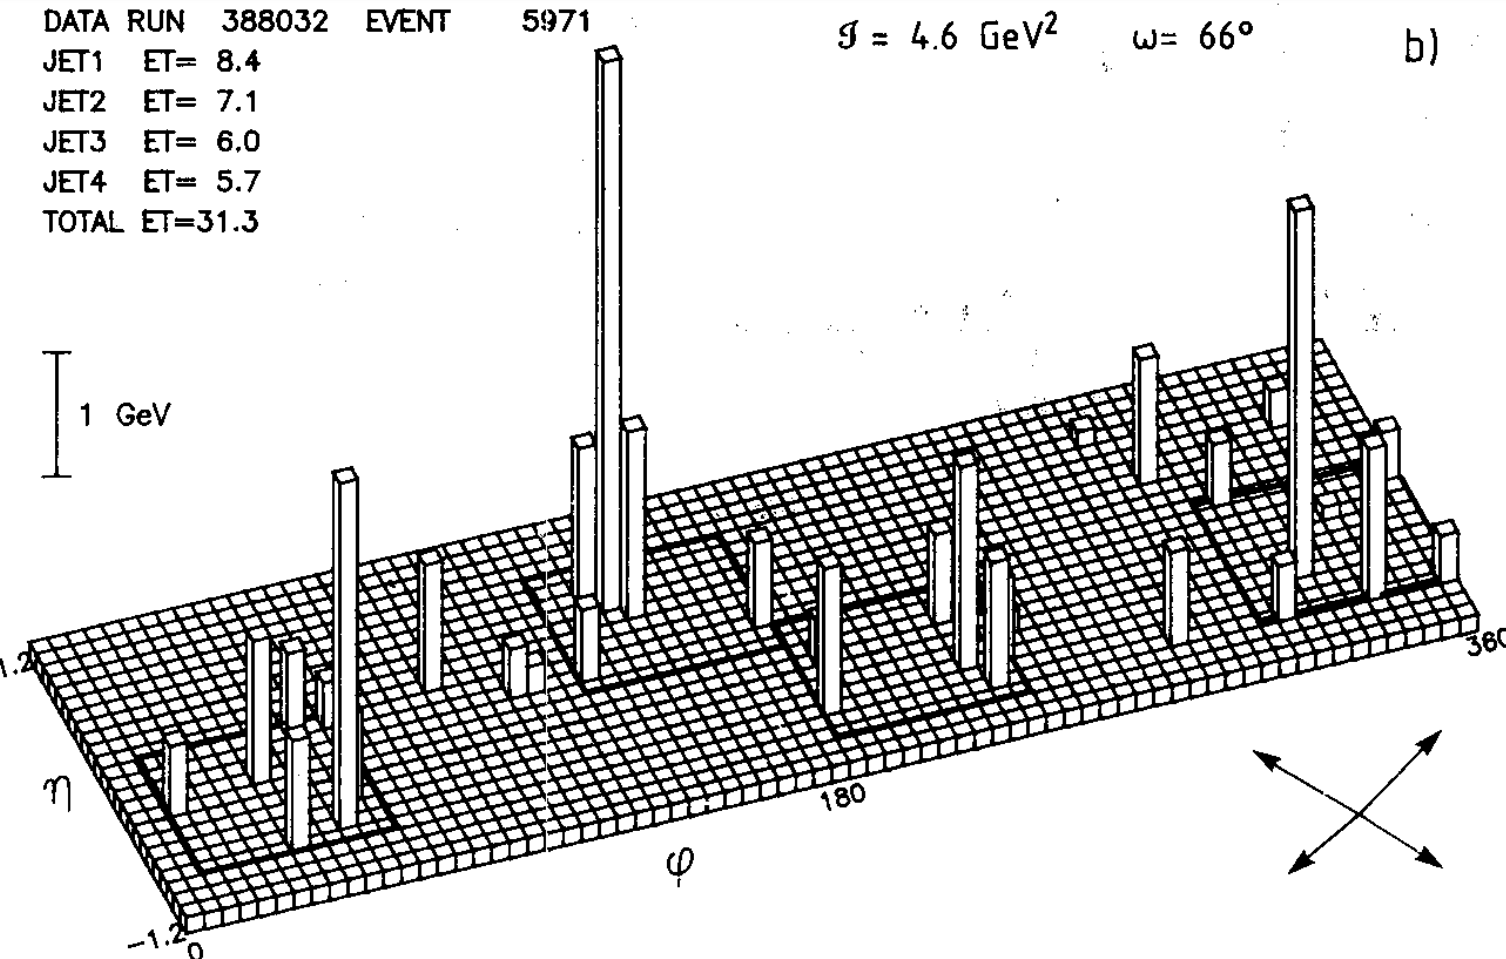
\includegraphics[width=.520\textwidth]{\imgpath/afs4jet.png}} 
\subfloat[][]{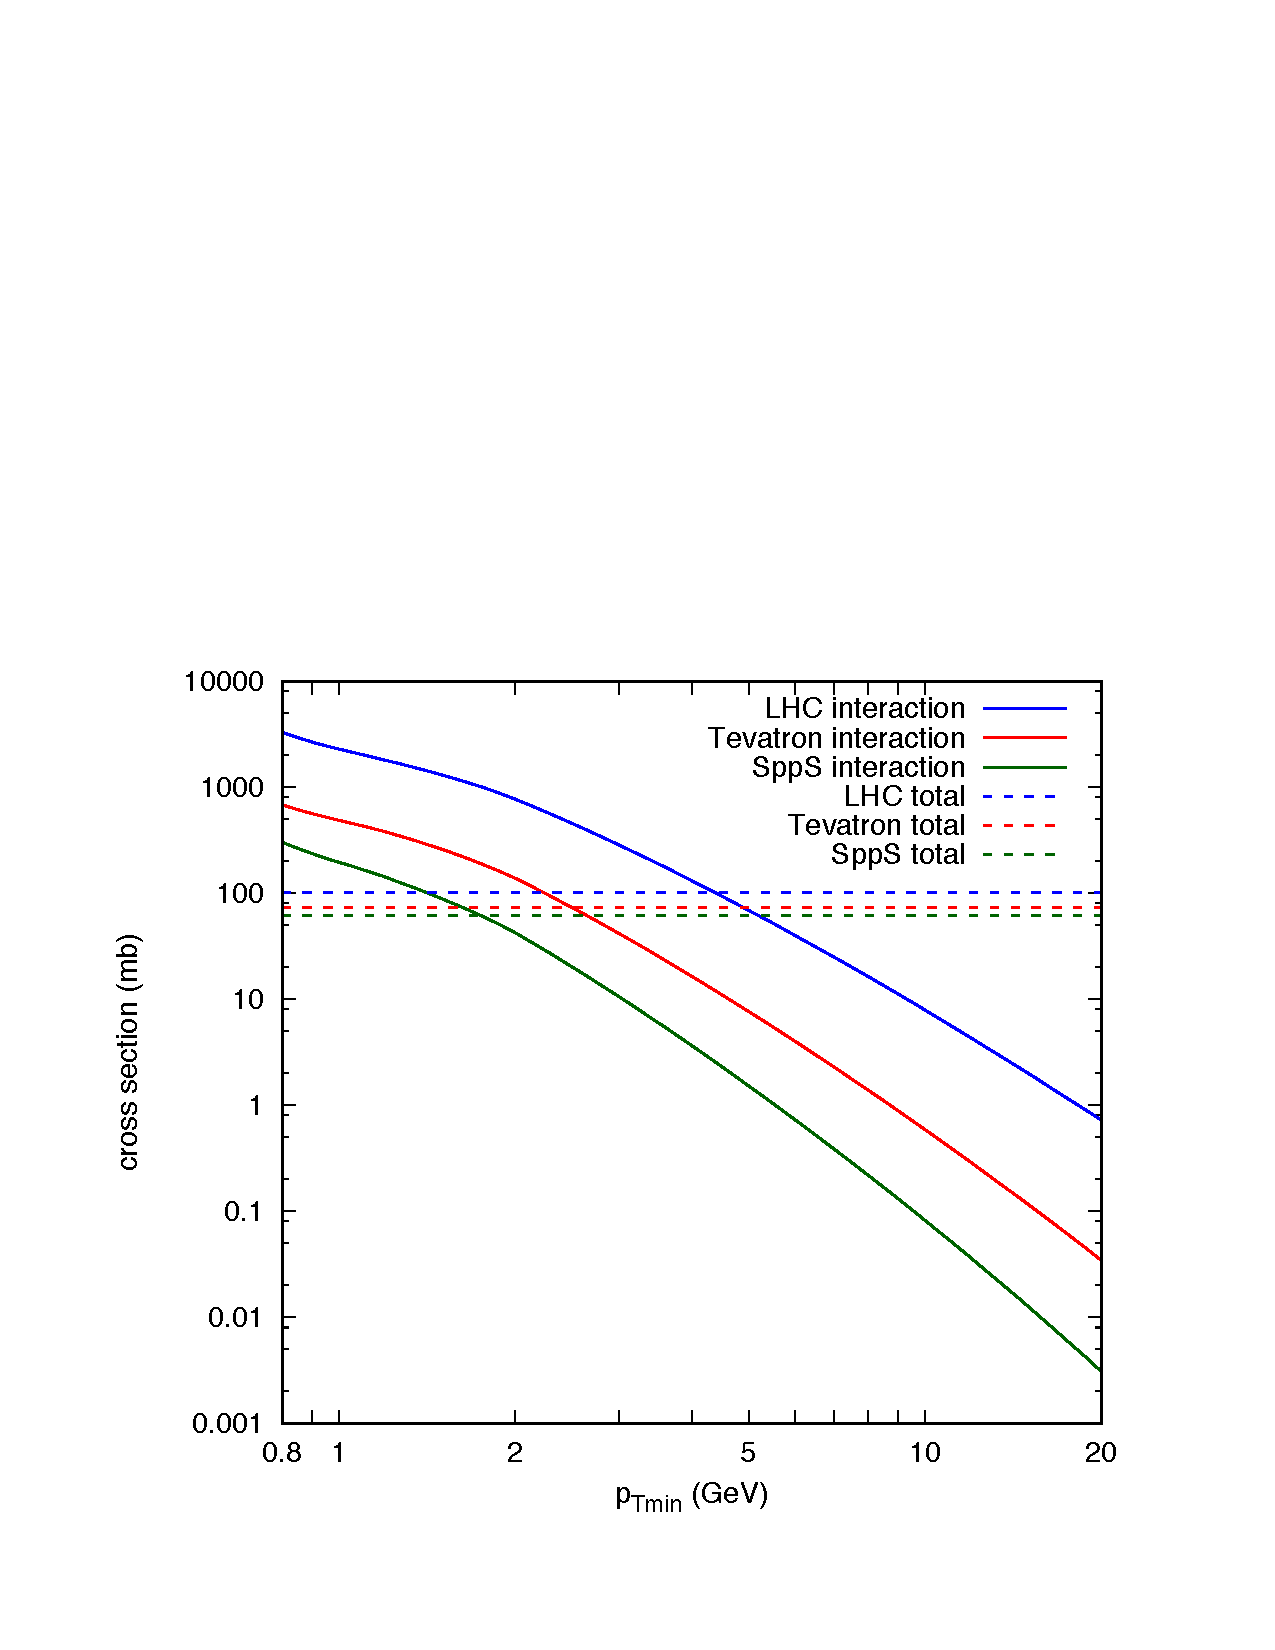
\includegraphics[width=.380\textwidth]{\imgpath/sigmampi.pdf}}
\caption{\textbf{(a)} Event display of an event with a 4-jet, where the pillars correspond to transverse energy deposits. \cite{akessonDoublePartonScattering1987} \textbf{(b)} Dependence of the integrated parton-parton cross section on the cutoff parameter $k_{\perp \mathrm{min}}$ for $\mathrm{Sp\bar{p}S}$ at \sppt{0.63}, Tevatron at \sppt{1.96}, and the LHC at \sppt{13}, modelled with Pythia. \cite{sjostrandDevelopmentMPIModelling2017}}
\label{fig:intro:afs4jet}
\end{figure}

These findings prompted further development of Regge theory and approaches that incorporated multiple pomerons, which were successful in describing the \Nch distributions. However, this approach is fully decoupled from descriptions of the perturbative primary scattering. Subsequently, much of the phenomenology related to multiple partonic interactions was developed within the framework of the Pythia MC event generator, which is discussed individually in Chapter~\ref{chap:colls} \cite{sjostrandDevelopmentMPIModelling2017}. However, nowadays, the relevance of the concept of MPIs in hadronic collisions extends beyond this generator. A scattering with double partonic interactions is illustrated in Fig.~\ref{fig:intro:dps}.

\begin{figure}[H]
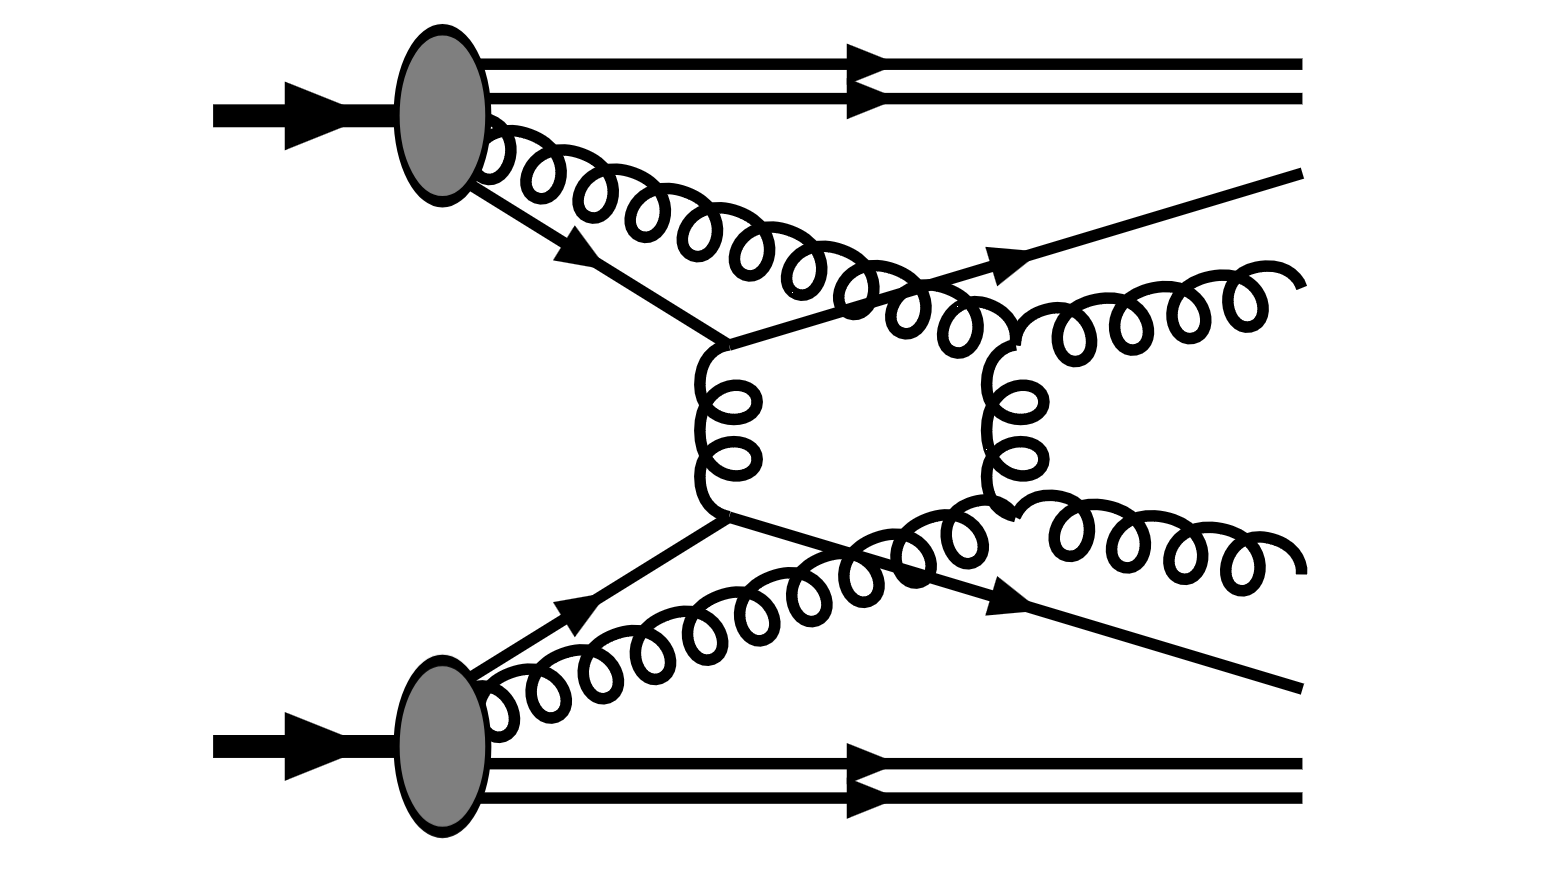
\includegraphics[height=7em]{\imgpath/dps.png}
\caption{Diagram showing a double partonic interaction, a case of $\nmpi=2$. \cite{prestelParticlePhysicsPhenomenology}}
\label{fig:intro:dps}
\end{figure}

In the Pythia approach, MPI are treated as additional perturbative scatterings. In QCD, the $2\to2$ cross section (dominated by the gluon exchange t-channel) diverges as $\propto \alpha^2_S(k_{\perp}^2)/k_{\perp}^4$, so a cutoff parameter $k_{\perp\mathrm{min}}$ must be introduced, and using (\ref{eq:intro:factorization}) leads to:
\begin{align}
\frac{d\sigma}{dk_{\perp}^2} &= \sum_{ij}\int dx_1 dx_2 f_i(x_1,\mu_F^2)f_j(x_2,\mu_F^2) \frac{d\hat{\sigma}^H_{ij}}{dk_{\perp}^2} \, , \\
\sigma_{\text{int}}(k_{\perp\text{min}}) &= \int_{k_{\perp\text{min}}^2}^{s/4} \frac{d\sigma}{dk_{\perp}^2}dk_{\perp}^2 \, .
\end{align}
The choice of cutoff can be tuned to experimental data, and for the $\mathrm{Sp\bar{p}S}$ energy of \sppg{630}, a value of around \gevc{1.6} was typical \cite{sjostrandDevelopmentMPIModelling2017}. The dependence of this parton-parton scattering cross section is shown in Fig.~\ref{fig:intro:afs4jet}.

The total pp cross-section, which is on the order of $100$~mb at \sppt{13}, is given by
\begin{align}
\sigma_{\mathrm{pp}} &= \sigma_{\mathrm{elastic}} + \sigma_{\mathrm{single \, dif.}} + \sigma_{\mathrm{double \, dif.}} + \sigma_{\mathrm{non-dif.}} \quad , 
\end{align}
where the inelastic cross sections $\sigma_\mathrm{inel} \approx \sigma_{\mathrm{double \, dif.}} + \sigma_{\mathrm{non-dif.}}$ corresponds to approximately 60\% of the total. The mean number of MPIs, \meannmpi, can be estimated using:
\begin{align}
\meannmpi (k_{\perp,\mathrm{min}}) = \frac{\sigma_{\mathrm{int}}(k_{\perp,\mathrm{min}})}{\sigma_{\mathrm{inel}}}
\end{align}

However, the actual treatment is more complex and involves considerations of other parameters such as the dampening factor $k_\perp^0$ to account for the confinement nature of partons, modifications of multiparton PDFs, energy-momentum conservation effects, $x$-dependent source geometry, and the intertwinedness of partonic evolutions.


In summary, MPIs represent several subcollisions that take place in an average pp collision with \pt scales of a few GeV. They are colour-connected to the beam remnants, which in the Lund model are represented by strings. Since a string with $\kappa = 1 \mathrm{GeV} /\mathrm{fm}$ yields, as a rule of thumb, approximately one hadron per unit rapidity, and the average pp collision at the LHC at \sppt{13} has $\langle \dndy \rangle \approx 6$, the typical number of partonic interactions is around six \cite{sjostrandDevelopmentMPIModelling2017}.

Finally, the observation of QGP-like phenomena in pp collisions at the LHC has renewed interest in MPI phenomenology, as discussed in the following chapter. Such observations do not contradict the concept of MPIs; rather, they suggest the possibility of incorporating collective behavior among the MPIs, such as interactions between strings, local modifications of string tensions, or, alternatively, the formation of a multipartonic state with QGP-like properties.

\subsection{Colour reconnection}

The incorporation of MPIs improved the description of the \Nch distributions and their dependence on $\sqrt{n}$. However, there were also observations of $\meanpt(\Nch)$ increasing as a function of \Nch, which could not be explained. More MPIs lead to more strings, which in turn leads to the production of more particles, but the \pt is mostly unaffected. This would predict a weaker dependence of \meanpt on \Nch, contrary to the data \cite{sjostrandDevelopmentMPIModelling2017}. The issue was resolved by implementing a possible color reconnection mechanism, which rearranges the color fields between partons.

\textit{TBA Insert diagrams of the processes!}

One can envision the following process:
\begin{align*}
e^+ e^- \rightarrow W^+ W^- \rightarrow q_1\bar{q}_2 q_3\bar{q}_4  .
\end{align*}
In this scenario, a color reconnection mechanism could rearrange the colour-connected $q_1\bar{q}_2$ and $q_3\bar{q}_4$ into $q_1\bar{q}_4$ and $q_3\bar{q}_2$ if it were energetically favourable, depending on the phase-space configurations. Measurements at LEP \cite{ElectroweakMeasurementsElectron2013} of this process have indeed shown that such final-state corrections must be taken into account to explain the data on $W$ masses and widths. They also reported that the reconnection probabilities for such events are on the order of $50\%$, further indicating that colour reconnection is an important factor to consider.

Pythia implements CR by minimizing the total length of strings in the system, analogous to minimising potential energy \cite{bierlichComprehensiveGuidePhysics2022}. This mechanism, illustrated in Fig.~\ref{fig:intro:cr}, explains the rising trend of $\meanpt$ as a function of \Nch: shorter strings imply fewer hadrons to split the transverse boost across, and the more MPI, the bigger this effect. Moreover, CR also helped describe the absolute value of \meanpt. With this approach, no further modifications of fragmentation parameters were necessary, in line with the concept of jet universality. However, it should be noted that there are various CR implementations and all rely on parameters obtained from tuning to data.

\begin{figure}[H]
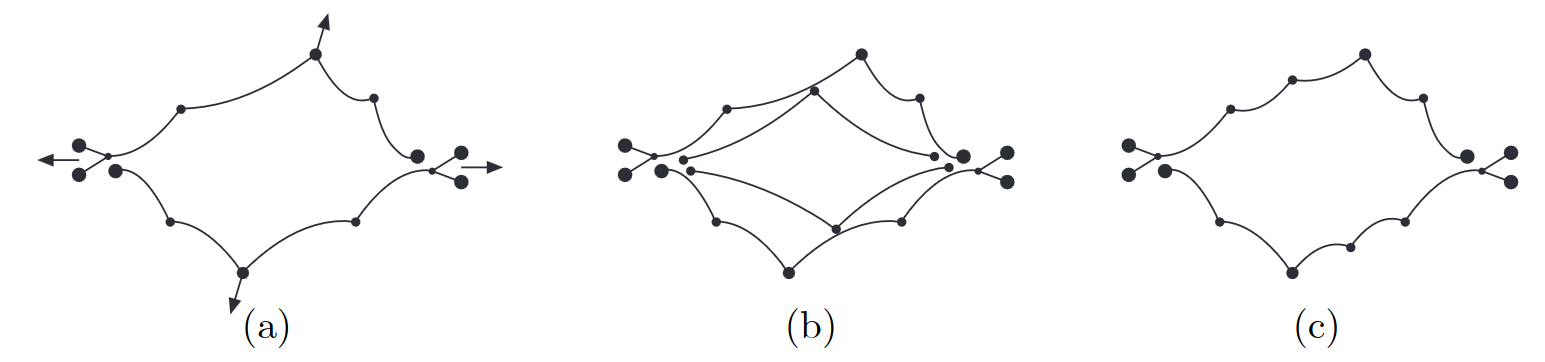
\includegraphics[height=7em]{\imgpath/cr.png}
\caption{Depiction of the CR process: \textbf{(a)} in a hard parton subcollision, the outgoing gluons are connected to the beam remnants through colour. Additional gluon kinks may occur through initial state radiation, which are ordered by rapidity. \textbf{(b)} A second hard scattering should theoretically result in two new strings connected to the remnants. \textbf{(c)} In order to minimise the total string length, gluons are colour reconnected. \cite{gustafsonMultipleInteractionsSaturation2009}}
\label{fig:intro:cr}
\end{figure}

It is also worth noting that the \pt boost acquired through color reconnection may depend on mass and whether a hadron is a baryon or meson, which somewhat mimics the hydrodynamic signatures of collective flow observed in AA collisions \cite{ortizColorReconnectionFlowlike2013}.

\section{Underlying event}\label{sec:intro:ue}

The underlying event (UE) in high-energy collisions refers to the additional hadronic activity that accompanies the primary hard scattering process, but is not directly related to it. This includes the fragmentation products of the beam remnants, ISR and FSR, as well as the effects of the previously discussed MPIs, and is visualised in Fig.~\ref{fig:intro:ue}. The UE (with its name coined at Tevatron \cite{cdfcollaborationChargedJetEvolution2002}) is typically characterized by a distribution of softer particles around and far outside of the hard process and was first observed at $\mathrm{Sp\bar{p}S}$ in the 1980s \cite{arnisonHadronicJetProduction1983}. These measurements saw a constant plateau of transverse energy $E_\mathrm{T}$ outside of the jet core, with its height independent of the jet energy.

\begin{figure}[H]
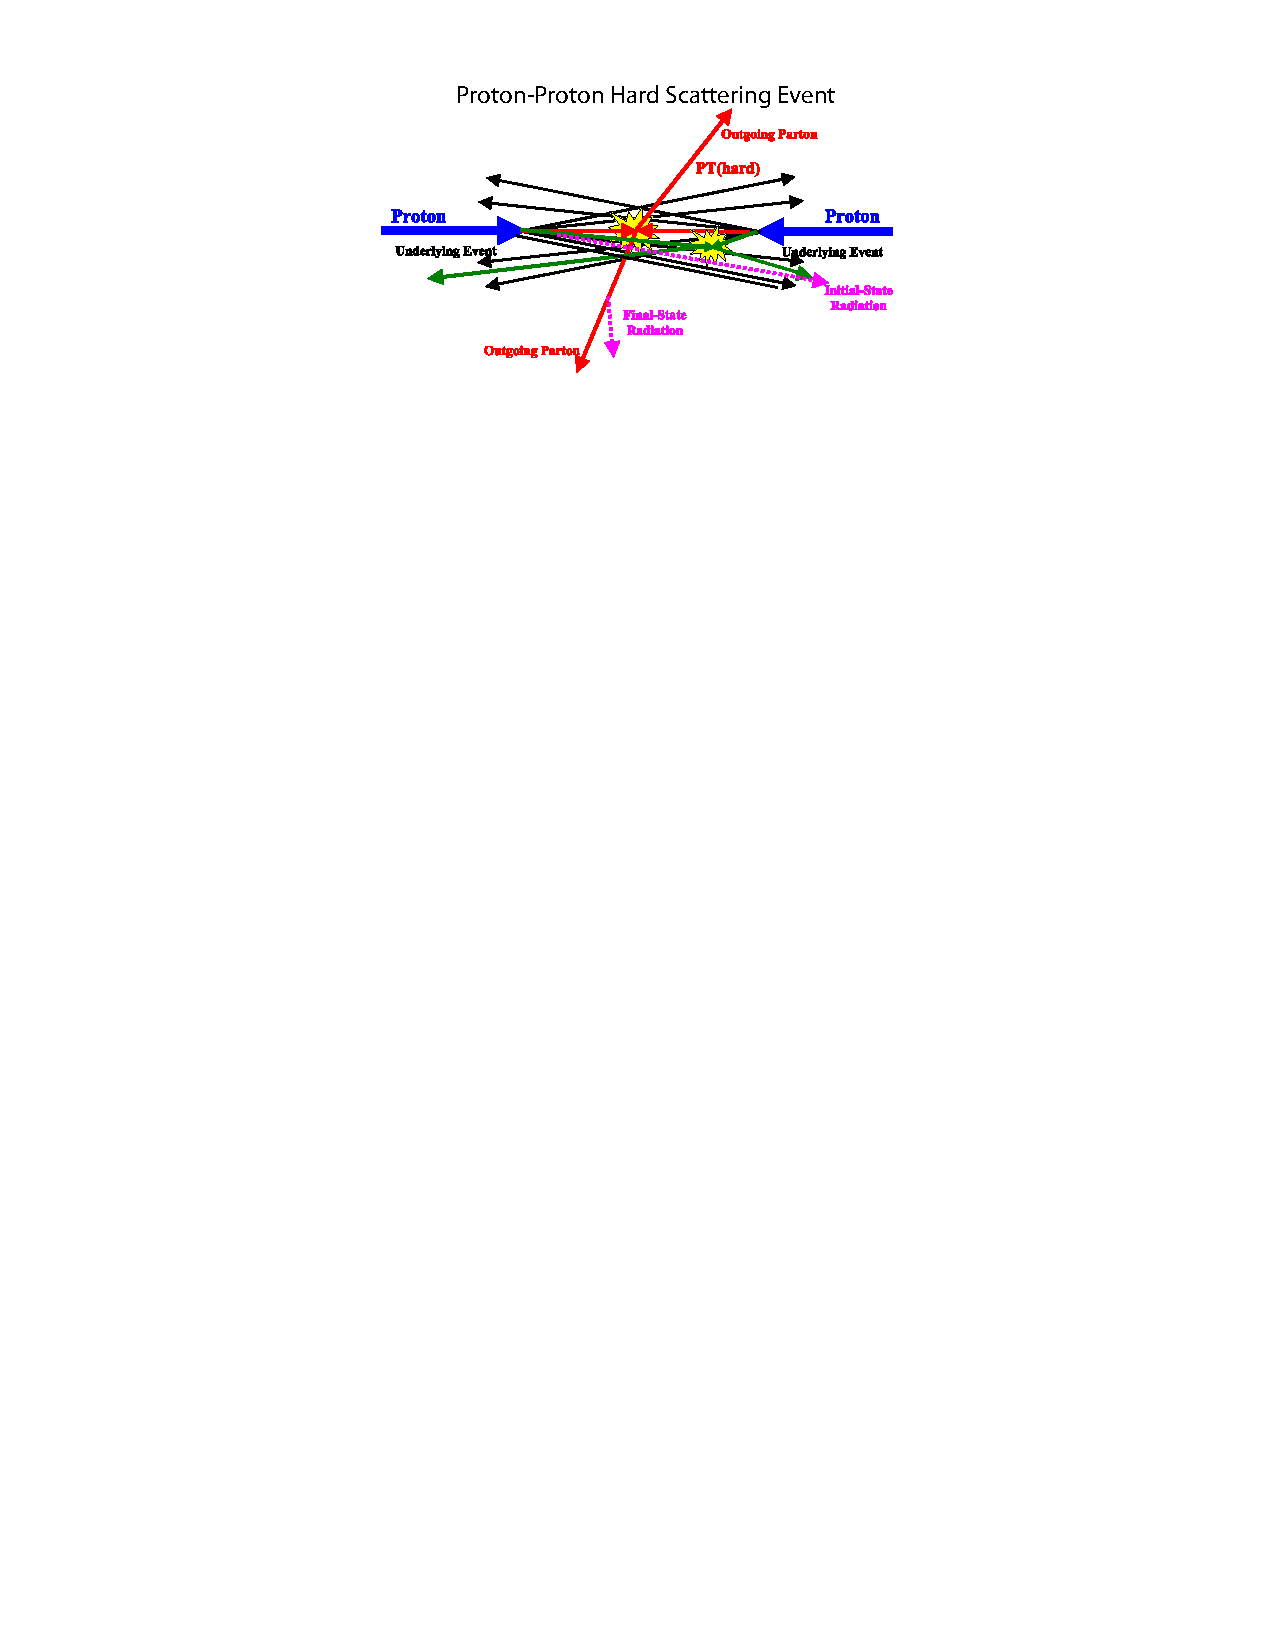
\includegraphics[width=.7\textwidth]{\imgpath/ue.pdf}
\caption{Cartoon illustrating a pp collision and its components: the hard scattering process, beam remnants, initial/final state radiation, and the MPIs. The last three contribute to the underlying event. \cite{cainesUnderlyingEventStudies2009, cdfcollaborationChargedJetEvolution2002}}
\label{fig:intro:ue}
\end{figure}

It is important to note that particle production in UE is different from the MB production, as it is biased by the presence of hard scattering. Additionally, the magnitude of the UE can fluctuate significantly from event to event.

\section{From hadrons to partons: deconfined QCD matter}

A simple argument can be made that confinement of quarks inside hadrons cannot be sustained when the density of partons is too large compared to that inside ordinary hadrons. Or alternatively, when the partonic kinetic energies are much larger than the confining part of the $q\bar{q}$ potential in (\ref{eq:intro:qqpot}). The following sections introduce some theoretical frameworks predicting the deconfinement of quarks and gluons. The calculations presented use natural units ($\hbar = c = k_B = 1$).

\subsection{Bag model of hadrons}

In this very naive approach \cite{detarBAGMODELSHADRONS1983, matonohaUpsilonMesonProduction2018}, hadrons are treated as spherical cavities (``bags") with radius $R$ of free massless quarks. These cavities exist in the non-perturbative QCD vacuum, which exerts a confining pressure $B$. The lowest-energy solution of the Dirac equation for the quarks, which in this case is $\slashed p \psi = 0$, is the $s_{1/2}$-state given by:
\begin{align}
\psi (r, t) = N \begin{pmatrix} j_0(\omega r) U \\ i \sigma \cdot \hat{r} j_1(\omega r) U \end{pmatrix} \exp (-i \omega t) \quad ,
\end{align}
where $N$ is a normalisation constant, $j_0$ and $j_1$ are spherical Bessel functions, $\omega$ is the quark energy, and $U$ the two-component spinor. The assumption that quarks are confined within the cavity volume represents the boundary conditions that the quark scalar density $\psi \bar{\psi}$ becomes zero at $r=R$, which is equivalent to $j_0(\omega R) = j_1(\omega R)$:
\begin{align}
j_0^2(\omega R) - \vec{\sigma} \cdot \hat{r} \vec{\sigma} \cdot \hat{r} j_1^2(\omega R) = 0 \\
j_0(\omega R) = j_1(\omega R) \quad ,
\end{align}
which happens when $\omega \approx \frac{2.04}{R}$. Thus, energy of the system can be given by
\begin{align}
E(R) \approx n_q \cdot \frac{2.04}{R} + \frac{4\pi}{3} B R^3 \quad .
\end{align}
Here, the first term represents the kinetic energy of $n_q$ quarks in the cavity and second term is the cavity volume energy. Gluon solutions should also be considered but are neglected in this approach. The first term acts to expand the cavity, whereas the second term acts to contract it. Finding an optimum of this energy with respect to $R$ leads to
\begin{align}\label{eq:intro:bagp}
B^{1/4} \approx \left( \frac{2.04 n_q}{4\pi} \right)^{1/4} \frac{1}{R} \quad .
\end{align}
Finally, assuming values for a proton, $R\approx 0.8$~fm, and three valence quarks $n_q=3$, the confining pressure can be approximated as $B^{1/4} \approx 206$~MeV. \cite{detarBAGMODELSHADRONS1983}

To relate the confining pressure to a critical temperature at which deconfinement occurs, $T_c$, one can assume a gas of relativistic massless fermions and bosons with energy density $\rho$ \cite{wongIntroductionHighEnergyHeavyIon1994, mcgreevyLectureNotesQuantum}. Using Stefan-Boltzmann law, the equation of state is,
\begin{equation}
P = \frac{1}{3} ( d_b + \frac{7}{8} d_f ) \rho = ( d_b + \frac{7}{8} d_f ) \frac{\pi^2}{90} T^4 \,
\end{equation}
where $d_b$ and $d_f$ are the degeneracy numbers for bosons and fermions, in this case gluons and quarks, respectively. Summing together possible colours, polarisations, and flavours for particles and antiparticles, one gets $d_b = 16$ and $d_f = 24$. Inserting the cavity pressure $B$ value calculated in (\ref{eq:intro:bagp}), $T_c$ can be estimated as approximately $145$~MeV.

\subsection{Lattice QCD}

Lattice QCD (LQCD) is a technique allowing calculation of processes involving the strong interaction in the non-perturbative regime, from first principles, without phenomenological assumptions. In this approach, the space-time continuum is discretised into a four-dimensional lattice, which allows QCD path integrals to be solved numerically. Smallest squares on the lattice are called \textit{plaquettes}, with the lattice links representing gluon fields and lattice sites representing quark fields. \cite{meyerLatticeQCDBrief2015}

Lattice calculations are computationally extremely intensive\footnote{In fact, in the past, LQCD was among important drivers of the advancement of GPU computing and it is also used as benchmark in high-performance computing \cite{bennettBSMBenchFlexibleScalable2016}.}, thus, a sufficiently coarse lattice spacing must be chosen to reduce computational costs and make the approach feasible. Often, simulations are also performed with unphysical quark masses (e.g.\ $m_q \sim m_\pi$), for the same reason. The results are then extrapolated using highly complex methods. Another limitation in LQCD is the so-called \textit{sign problem}, discussed in detail for instance in Ref.~\cite{nagataFinitedensityLatticeQCD2022}, which arises when evaluating highly oscillatory complex integrals in finite-density environment.

Despite its challenges, LQCD has been successful in various predictions, notably, the \textit{ab initio} calculation of the mass of neutron (uud) using the mass of $\Omega$ (sss) as an input \cite{durrInitioDeterminationLight2008}. Furthermore, it allows for the calculation of thermodynamics of QCD matter and predicts its equation of state, as well as a phase transition at $T_c \approx 150$~MeV \cite{petreczkyLatticeQCDNonzero2012, bazavovEquationStateFlavor2014}, which is usually identified with the formation of quark-gluon plasma QGP, discussed in Chapter~\ref{chap:colls}. The dependence of energy density and pressure on temperature can be seen in Fig.~\ref{fig:intro:eos}.

\begin{figure}[H]
\subfloat[][]{\adjustbox{valign=m}{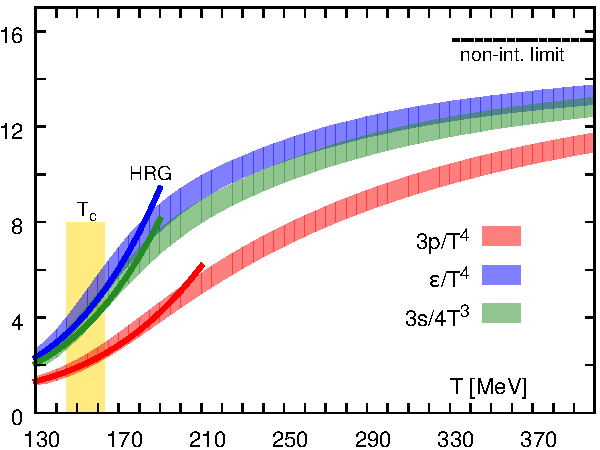
\includegraphics[width=.40\textwidth]{\imgpath/eos.pdf}}}\hspace{1.5em}%
\subfloat[][]{\adjustbox{valign=m}{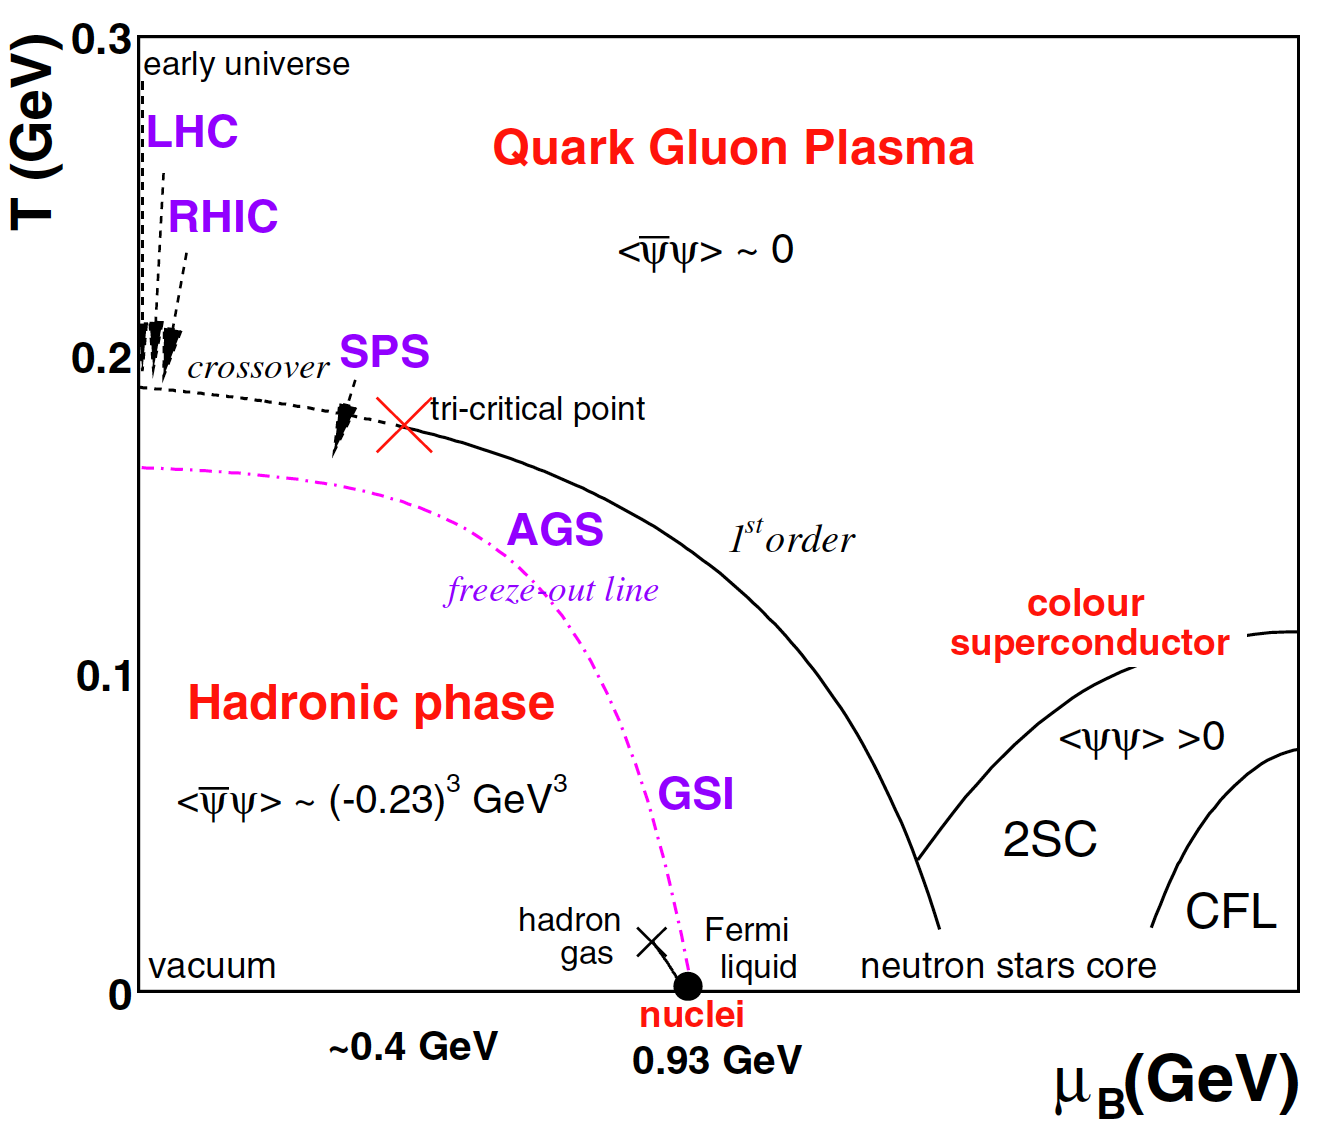
\includegraphics[width=.50\textwidth]{\imgpath/phasediagram.png}}}
\caption{\textbf{(a)} Dependence of the pressure (red), energy density (blue), and entropy density (green) on temperature, determined with LQCD. \cite{bazavovEquationStateFlavor2014} \textbf{(b)} Phase diagram of QCD matter. \cite{pasechnikPhenomenologicalReviewQuark2017}}
\label{fig:intro:eos}
\end{figure}

\subsection{QCD phase diagram, chiral symmetry restoration}

Phase transitions of QCD matter are investigated to explore the QCD phase diagram with respect to temperature $T$ and baryon chemical potential $\mu_B$, which corresponds to net baryon density. Figure~\ref{fig:intro:eos} visualizes the different areas of the QCD phase diagram probed by various experiments \cite{pasechnikPhenomenologicalReviewQuark2017}. Measurements of Pb-Pb collisions at the LHC access high $T$ and almost zero $\mu_B$, as the nucleons of ultrarelativistic Pb nuclei escape the interaction volume before the plasma develops, and the high energy subsequently leads to a sizable baryon production balanced by anti-baryons due to conservation laws. Experiments studying collisions of slower and heavier nuclei reach higher $\mu_B$ regions.

Furthermore, looking back at the QCD Lagrangian in (\ref{eq:intro:lqcd}) and neglecting quark current masses $m_{u,d}\to 0$, it can be seen that it is invariant when switching the up and the down quark, corresponding to a SU($2$) isospin symmetry. This allows the fermion fields to be rewritten in terms of their left and right chiralities and the QCD Lagrangian then exhibits a larger \textit{chiral symmetry}.

However, it is known that the vacuum expectation value of a $q\bar{q}$ state is much larger than the current masses $m_{u,d}$:
\begin{equation}
\langle 0 | q \bar{q} | 0 \rangle = \langle 0 | u\bar{u} + d \bar{d} | 0 \rangle \approx (250 \, \mathrm{MeV} )^3 \quad ,
\end{equation}
where the value is taken from average masses of light flavour mesons. This means that the QCD vacuum spontaneously breaks the chiral symmetry. \cite{sazdjianIntroductionChiralSymmetry2017}

It can be expected that in the plasma of deconfined quarks and gluons, chiral symmetry is \textit{restored} \cite{gottliebEstimatingChiralsymmetryRestoration1987, xuChiralSymmetryRestoration2023}. This is actively studied in AA collisions, for example in searches of the so-called chiral magnetic effect \cite{starcollaborationSearchChiralMagnetic2021} or degeneracy of normally chiral partners \cite{hohlerRmesonMeltingCompatible2014}, such as the $\rho$ ($J^P=1^-$) and $a_1$ ($J^P=1^+$) states.

%\section{Implications of high-activity QCD research}
%
%Understanding the early universe: The QGP is believed to have existed in the first few microseconds after the Big Bang. Studying QGP can provide insight into the behavior of matter and the formation of the universe
%Understanding of fundamental physics: QGP is a unique state of matter that is not well understood. Studying QGP can provide insight into the behavior of quarks and gluons, which are the building blocks of matter.
%Developing a deeper understanding of strong interactions: The strong nuclear force is one of the four fundamental forces of nature. Studying QGP can provide insight into the behavior of this force and its interactions with matter.
\chapter{Collisions of particles at high energies}
\begin{tcolorbox}[colback=yellow!10!white,colframe=red!50!black,fonttitle=\scshape,
  titlerule=0pt,
  title={\refstepcounter{exa}example~\theexa: Title of Example},
  title style={fill=yellow!10!white},
  coltitle=white, %red!50!black
  drop shadow]
  Hi, i am a yellow example
  \begin{center}
    \centering
    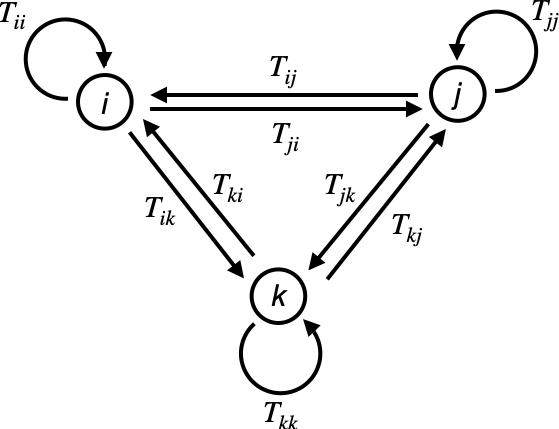
\includegraphics[width=0.99\textwidth]{figures/graph.png}
    \label{example:dice_entropy}
  \end{center}
\end{tcolorbox}
In example \ref{example:dice_entropy}

\begin{thesisbox}{The important concept}
\blindtext
\end{thesisbox}
\blindtext
\chapter{QCD phenomena in high energy collisions}
\blindtext
\chapter{Phenomenological models of hadronic collisions}
\blindtext

\part{Experimental Setup and Methodology}
\chapter{Large Hadron Collider}
\def \imgpath {"./figures/lhc"}

\textit{This chapter is currently unfinished and needs a lot of work.}

\section{European Organisation for Nuclear Research}
CERN, located near Geneva, Switzerland, is an esteemed scientific institution dedicated to the study of particle physics, nuclear physics, and related fields. Established in 1954 by a consortium of European countries, it currently has 23 member states and collaborates with over 50 countries worldwide. Its research endeavors focus on advancing our understanding of the fundamental particles and forces that govern them.

One of the most significant and celebrated discoveries made by CERN is the Higgs boson, a particle that confers mass to other particles and is a crucial component of the Standard Model of particle physics. This discovery was made in 2012 by the ATLAS and CMS experiments, two of the four main experiments at CERN's Large Hadron Collider (LHC), the world's largest and most powerful particle accelerator.

Apart from the LHC, CERN houses several research facilities, including the Proton Synchrotron and the Super Proton Synchrotron, that provide beams of particles for a wide range of experiments. %In sum, CERN is a preeminent international center for pioneering research in particle physics and allied domains, and its findings and technological advancements have contributed substantially to our understanding of the universe. Furthermore, it embodies the potency of international collaboration and cooperation in scientific exploration.

\section{Large Hadron Collider (LHC)}

The Large Hadron Collider (LHC) is a particle accelerator that utilizes a circular tunnel with a circumference of 27 kilometers to accelerate beams of protons or heavy ions to high energies and collide them at four separate experimental locations. The LHC operates on the principle of accelerating these beams to nearly the speed of light through a series of superconducting magnets and then directing them to collide with each other at specific points along the circular path.

The LHC's superconducting magnets are cooled to temperatures close to absolute zero (-271.3 degrees Celsius) to maintain their superconducting state, allowing them to guide and focus the particle beams as they travel along the circular path. These magnets produce a strong magnetic field that keeps the particle beams on their circular trajectory and causes them to bend as they pass through the magnetic field. By adjusting the strength of the magnetic field, the LHC can control the curvature of the particle beams and ensure that they collide at the designated interaction points.

The LHC's acceleration process occurs in a series of stages, starting with a source of particles that are injected into a linear accelerator (LINAC). The LINAC accelerates the particles to an energy of a few million electronvolts (MeV) before passing them to a circular accelerator called a Booster. The Booster further accelerates the particles to an energy of 1.4 billion electronvolts (GeV) before injecting them into the Proton Synchrotron (PS).

The PS is a circular accelerator that increases the energy of the particles to 25 GeV before injecting them into the Super Proton Synchrotron (SPS). The SPS is a larger circular accelerator that further accelerates the particles to 450 GeV before finally injecting them into the LHC. Once inside the LHC, the particles are accelerated to their final energy and directed to collide at the designated interaction points.

The collisions at the LHC produce a shower of subatomic particles that are captured and analyzed by the LHC's four primary detectors: ATLAS, CMS, LHCb, and ALICE. These detectors are designed to measure the properties and trajectories of the particles produced by the collisions and provide valuable insights into the fundamental nature of matter and the universe.

Overall, the operational principle of the LHC is based on the precise control of the particle beams through a series of superconducting magnets and accelerators to produce high-energy collisions that enable cutting-edge research in particle physics.

The LHC tunnel is situated approximately 100 meters underground, in a tunnel that was previously used by the Large Electron-Positron Collider (LEP). It has a diameter of 3.8 meters and houses over 1,600 superconducting magnets. The collider operates for periods of several months at a time, with periods of downtime in between for maintenance and upgrades.

TBA Luminosity, bunches, Van der Meer scans

\begin{figure}%[!h]
\centering%
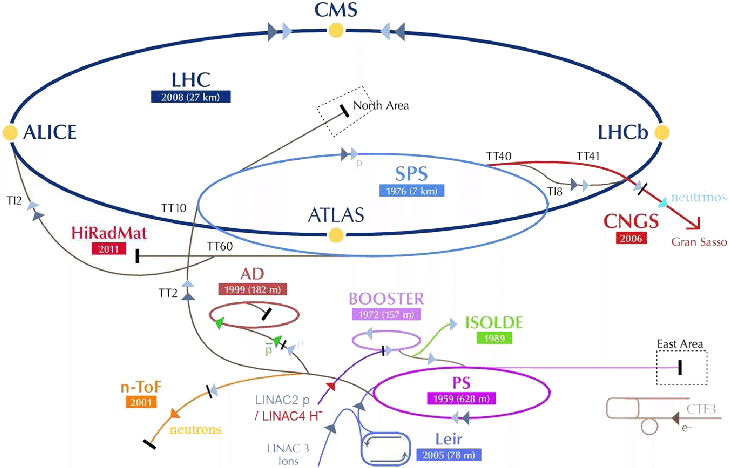
\includegraphics[width=.7\textwidth]{\imgpath/cern.png}
\caption{TBA.}
\label{fig:experiment:cern}
\end{figure}


\begin{figure}%[!h]
\centering%
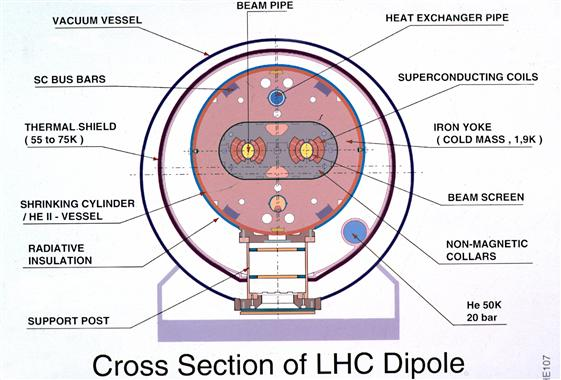
\includegraphics[width=.7\textwidth]{\imgpath/dipole.jpg}
\caption{TBA.}
\label{fig:experiment:cern}
\end{figure}
\chapter{The ALICE Detector}
\def \imgpath {"./figures/alice"}


\begin{figure}%[!h]
\centering%
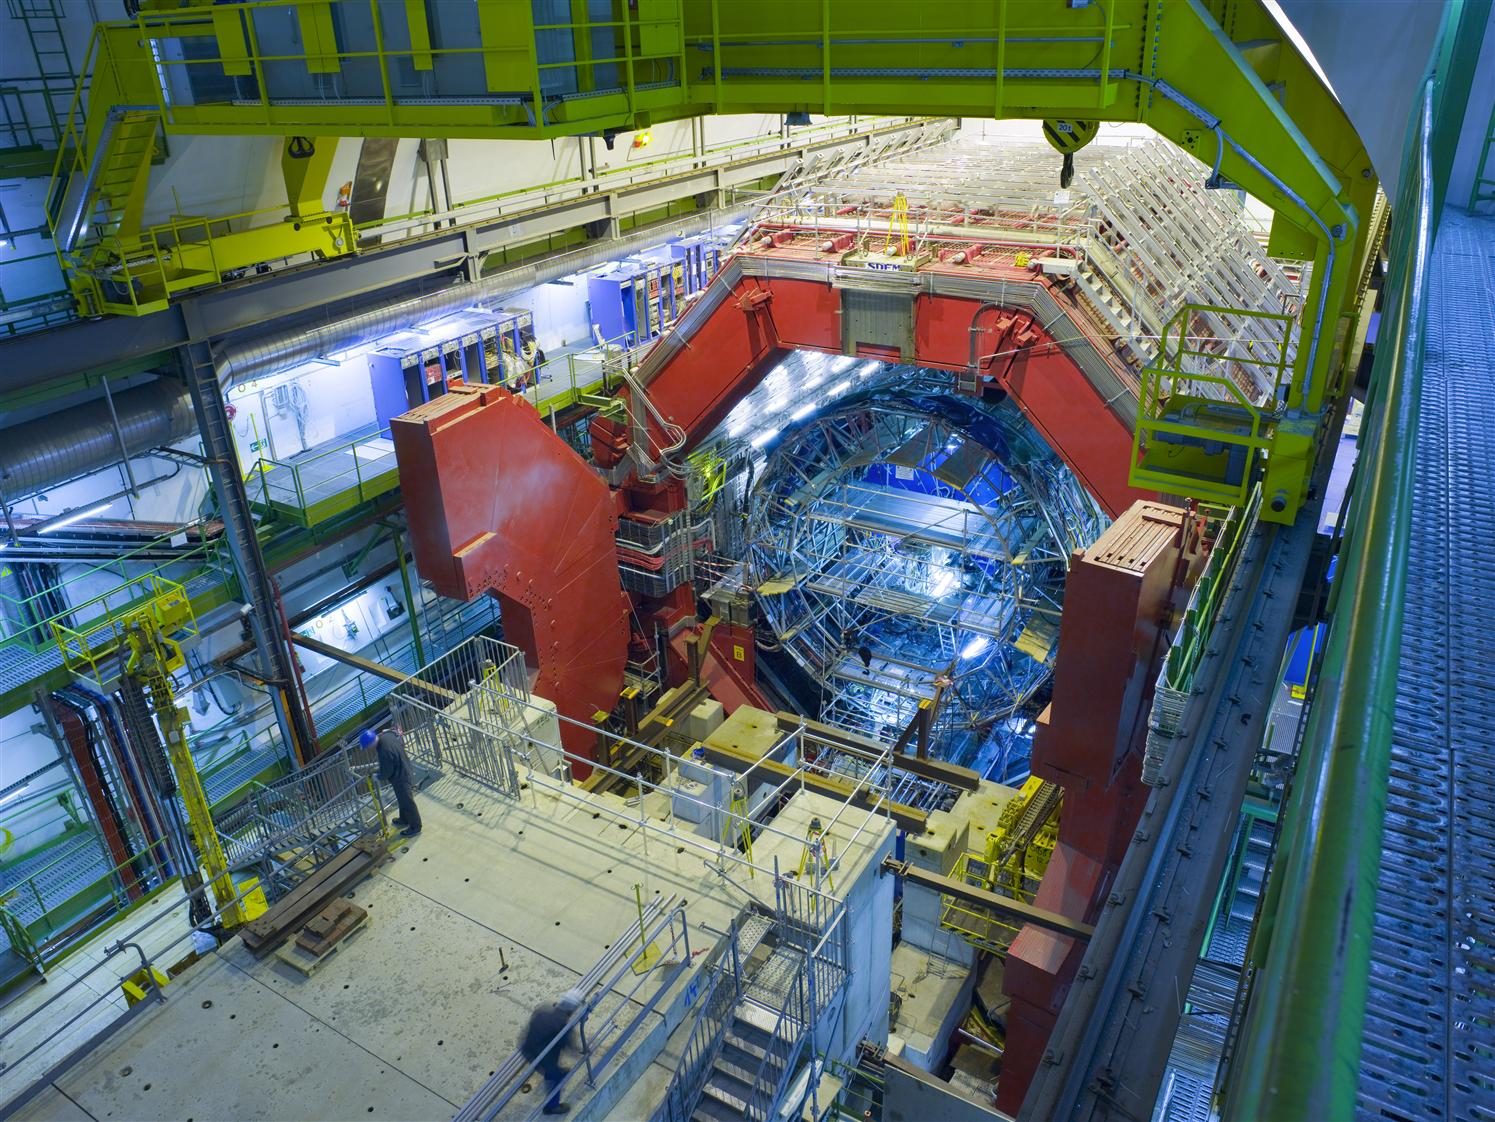
\includegraphics[width=.7\textwidth]{\imgpath/alicephoto.jpg}
\caption{TBA.}
\label{fig:experiment:cern}
\end{figure}

The ALICE (A Large Ion Collider Experiment) is one of four major detectors located at the Large Hadron Collider (LHC) at CERN. The ALICE detector is designed to study the properties of the quark-gluon plasma (QGP), a state of matter that existed a few microseconds after the Big Bang.

The ALICE detector consists of several sub-detectors that work together to capture and analyze the particles produced by the collisions at the LHC. The central component of the ALICE detector is the Time Projection Chamber (TPC), a large cylinder filled with a gas mixture that is used to detect the charged particles produced by the collisions. The TPC measures the position, momentum, and energy of the particles, allowing scientists to reconstruct their trajectories and identify the different particle species.

In addition to the TPC, the ALICE detector also includes several other sub-detectors, such as the Inner Tracking System (ITS), the Transition Radiation Detector (TRD), and the Time-Of-Flight (TOF) detector. The ITS is a high-precision tracking detector that is used to measure the trajectories of charged particles produced in the collisions. The TRD is used to identify electrons and measure their energy. The TOF detector measures the time-of-flight of particles and is used to determine their momentum.

\begin{figure}%[!h]
\centering%
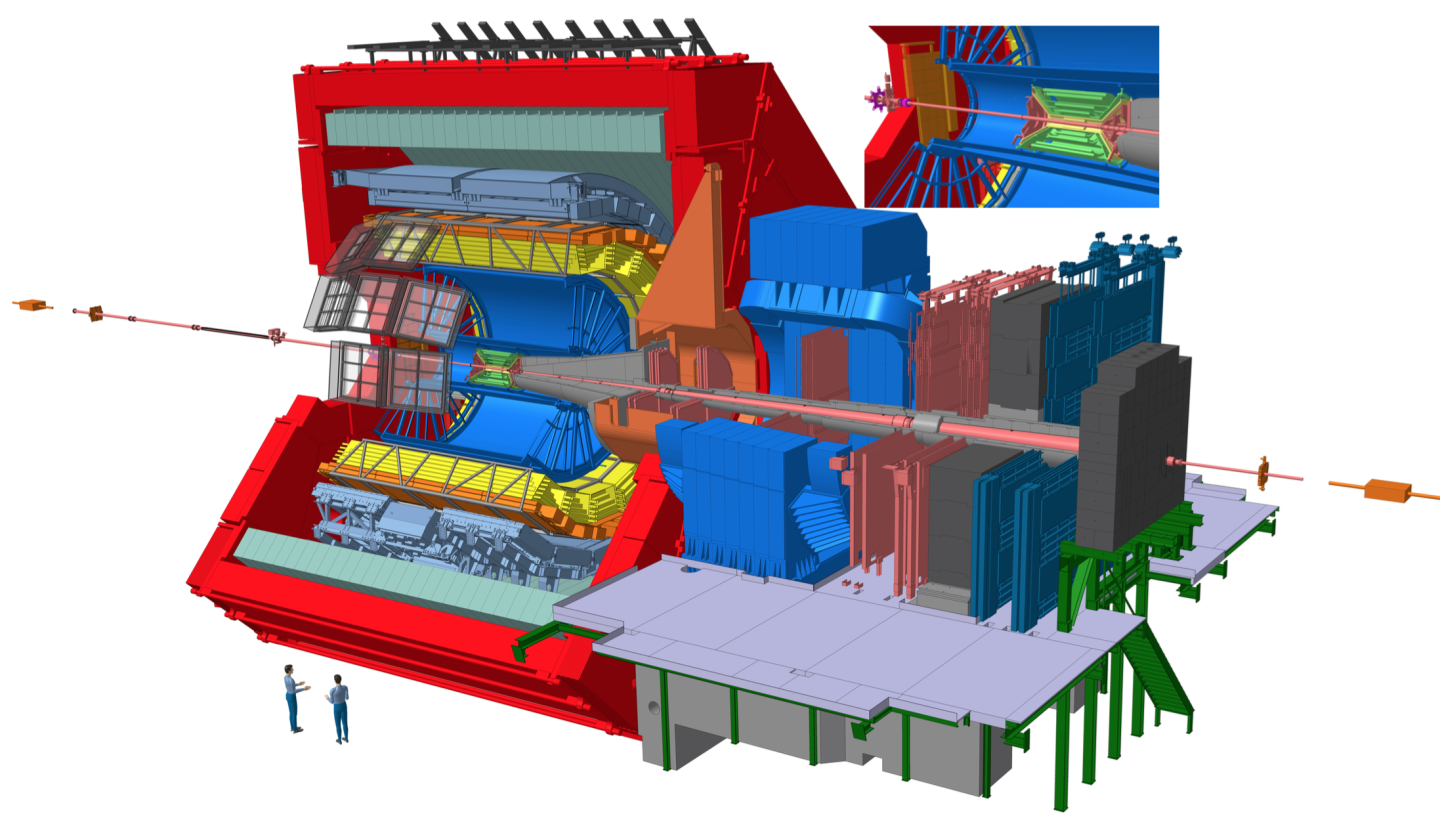
\includegraphics[width=.7\textwidth]{\imgpath/alicescheme2.png}
\caption{TBA.}
\label{fig:experiment:cern}
\end{figure}


\begin{figure}%[!h]
\centering%
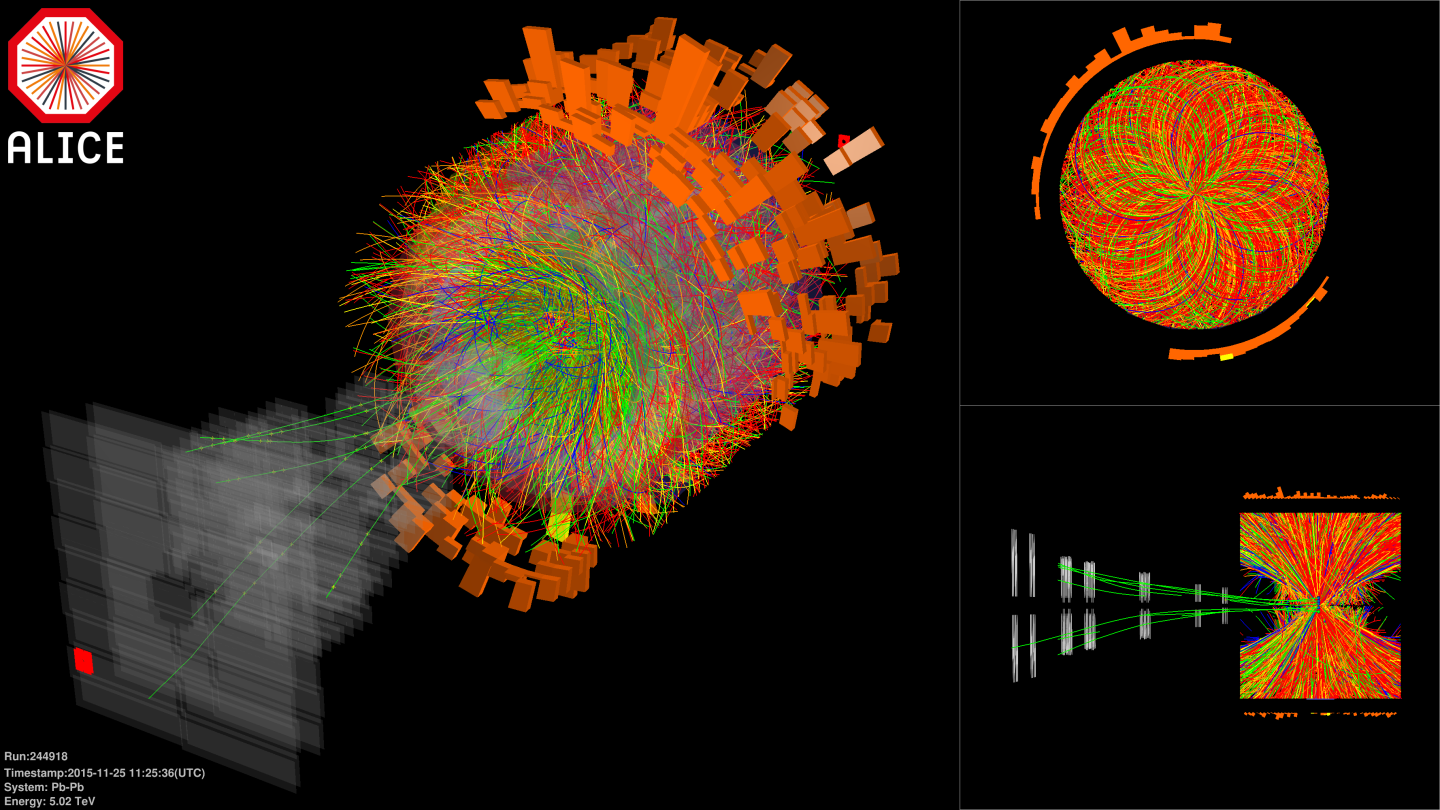
\includegraphics[width=.7\textwidth]{\imgpath/aliceevent.png}
\caption{TBA.}
\label{fig:experiment:cern}
\end{figure}

\section{Time Projection Chamber}

The TPC works by filling the cylinder with a gas, typically a mixture of helium and carbon dioxide, and applying an electric field to create a uniform drift velocity for the charged particles. As the particles move through the gas, they ionize the atoms, creating free electrons and ions. The electrons are then attracted to a central anode, where they are detected and used to reconstruct the particle tracks.

The TPC has a number of advantages over other types of detectors. For one, it is able to provide precise measurements of the position and momentum of the charged particles, which allows scientists to study the behavior of quark-gluon plasma and other forms of matter at extremely high temperatures and densities. The TPC is also able to reconstruct the tracks of thousands of particles produced in a single collision, which provides a comprehensive view of the event.

The TPC in the ALICE experiment is particularly advanced, with over 500,000 readout channels and a sensitive volume of over 90 cubic meters. It is able to operate at high collision rates, with a maximum readout rate of 50 kHz. The TPC also has a number of innovative features, such as a gating system that allows the detector to operate in the presence of large magnetic fields, and a continuous calibration system that ensures high data quality.


\begin{figure}%[!h]
\centering%
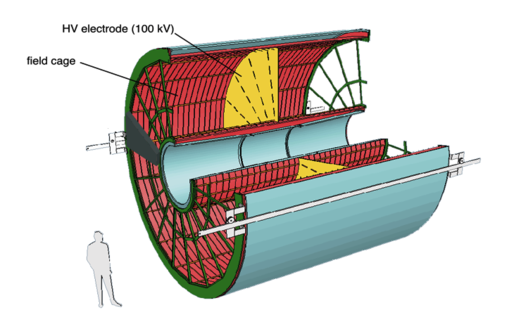
\includegraphics[width=.7\textwidth]{\imgpath/alicetpc.png}
\caption{TBA.}
\label{fig:experiment:cern}
\end{figure}


\section{Inner Tracking Systems}

The ITS is another tracking detector in the ALICE experiment, located closer to the collision point than the TPC. It is designed to provide precise measurements of the position of charged particles as they are produced in the collisions. The ITS consists of six layers of silicon detectors, which provide high-resolution measurements of the position and momentum of the particles. The ITS is particularly useful for studying the very early stages of the collision, where the particles are produced in a very small volume and with high energies.


\begin{figure}%[!h]
\centering%
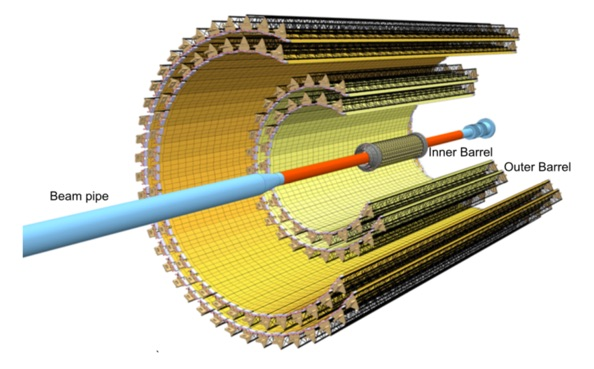
\includegraphics[width=.7\textwidth]{\imgpath/aliceits.jpg}
\caption{TBA.}
\label{fig:experiment:cern}
\end{figure}

\chapter{Events, Vertices, Tracks, and Particles}
\blindtext

\part{Author's measurements}
\chapter{Reconstruction of neutral strange particles with ALICE}
\def \imgpath {"./figures/analysis"}
Hadrons \KOs and \LA (\AL) are unstable neutral primary particles that usually decay within the volume of the detector through the weak interaction. Their mean lifetimes are $\sim \cmc{2.7}$ and $\sim \cmc{7.9}$, respectively.\cite{alicecollaborationALICEDefinitionPrimary2017} Their dominant decay channels, which are also used for their measurement, are:
\begin{align}
\KOs &\rightarrow \pip \, \pim \\
\LA &\rightarrow \p \, \pim \\
\AL &\rightarrow \pbar \, \pip \, \, .
\end{align}
Because of how these hadrons' decay topologies appear in the detector (an undetectable neutral particle decaying into a V-shaped pair of detectable tracks), they are commonly nicknamed \VOs \footnote{Not to be confused with \VOA and \VOC---the forward calorimeters in ALICE, or \VOM---the related multiplicity estimator using the calorimeters' signal.}. 

\section{Analysed datasets}
TBA
Description of data, collection years, some QA
Monte Carlo
The Monte Carlo data are simulated using a physics event generator (in this measurement, Pythia 8\cite{bierlichComprehensiveGuidePhysics2022}) and a model describing the propagation of particles through the detector environment (GEANT\cite{brunGEANTDetectorDescription1993,agostinelliGEANT4aSimulationToolkit2003}). 

\section{Identification of \VOs using ALICE}\label{sec:ana:cuts}
A centrally developed ALICE algorithm, the ALICE \VO finder, is used to collect suitable \VO candidates from pairs of oppositely charged tracks  with the relevant topology. This typical topology is illustrated in Fig.~\ref{fig:analysis:v0decay.} %More details here and cite
Additional selection criteria (``cuts") are further applied to suppress the background among those candidates. These include:
\begin{itemize}
\item cuts on kinematics of the mother and the daughters,
\item constraints on the topology of the decay,
\item constraints on the reconstruction quality of the daughter tracks,
\item cuts on the specific ionisation energy loss of the daughters, 
\item rejection of contributions from pile-up using ``fast detector" information,
\item rejection of other competing \VO candidates based on their invariant mass.
\end{itemize}
The full list of used cuts is listed in Tab.~\ref{tab:analysis:v0cuts}.

\begin{figure}
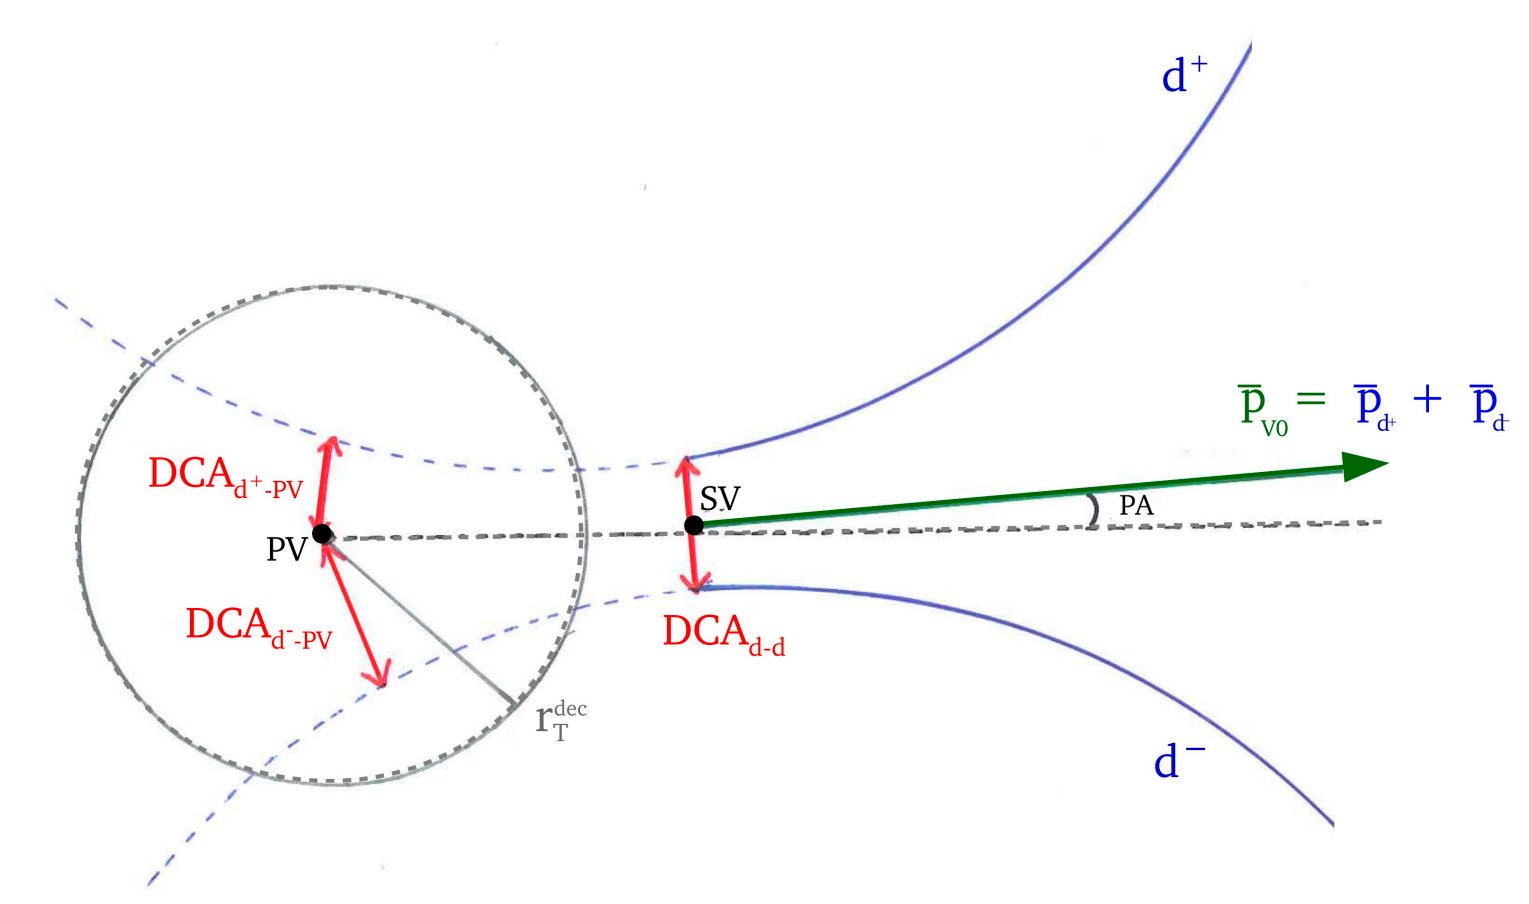
\includegraphics[width=.75\textwidth]{\imgpath/analysis_v0decay.png}
\caption{Typical topology of \VO decay. PV stands for primary vertex, SV for secondary vertex. \citep[p.~102]{tuvathesis}}
\label{fig:analysis:peakfit}
\end{figure}

\begin{table}[h!]
\begin{center}
\caption{Cuts used in the identification of the \Ks , \LA , and \AL particles.}
\label{tab:analysis:v0cuts}
\begin{tabular}{|l|c|}
\hline
 \parbox[b][1.1em]{1em}{}Cut Variable & Cut Value for \Ks (\LA , \AL ) \\ \hline
 
 \multicolumn{2}{l}{\parbox[b][1.2em]{1em}{}Topology} \\ \hline
\parbox[b][1.1em]{1em}{}\VZ pseudorapidity & $-0.8 < \eta < 0.8$ \\
Transverse momentum & $1.0 < \pt < 25.0$ \gev \\
\VZ DCA  & $\mathrm{DCA}^\mathrm{d-d} < 1.0$ \\
Pointing angle & $\cos \mathrm{PA} > 0.97 (0.995)$ \\
Decay radius & $0.5~\mathrm{cm} < R_{xy}$ \\ \hline

\multicolumn{2}{l}{\parbox[b][1.2em]{1em}{}Daughter Tracks Selection} \\ \hline
\parbox[b][1.1em]{1em}{}DCA of daughters to PV &  $\mathrm{DCA}^\mathrm{d-PV}_{xy} > 0.06$ cm \\
TPC PID of daughters & $< 5 \, \sigma$\\
Track pseudorapidity & $-0.8 < \eta < 0.8$ \\
TPC crossed rows & $N_\mathrm{cr} > 70$ \\
TPC crossed rows to findable ratio & $N_\mathrm{cr}/N_\mathrm{f} > 0.8$ \\ \hline

\multicolumn{2}{l}{\parbox[b][1.2em]{1em}{}Candidate Selection} \\ \hline
\parbox[b][1.1em]{1em}{}Proper lifetime (transverse) & $( \, R_{xy} \times m_{(\LA , \AL) } / p_\mathrm{T} < 30$~cm$ \,)$  \\
Competing mass & $ > 4\, \sigma$ \\ \hline


\end{tabular}
\end{center}
\end{table}
% Cuts need more description

\section{Signal extraction}
The \VO signal is separated from the background in distributions of \Minv in several \pt intervals using the so-called sideband method. Assuming the signal peaks around $\dMassVO=\Minv-\MVO=0$ and approximating the background in this region as linear, the subsequent procedure is followed:
\begin{enumerate}
\item the sideband regions are defined. The \Minv spectra are fitted in the $-0.03<\Minv<\gevcc{-0.03}$ interval using a \Chisq-fit with the distribution
\begin{align}
f = [0] + [1]\cdot\Minv + [2] \cdot \Gaus (\mu,\sigma_1^2) + [3] \cdot \Gaus (\mu,\sigma_2^2) \, \, ,
\end{align}
where \Gaus is a Gaussian distribution. This is done in all \pt bins and illustrated in Fig.~\ref{fig:analysis:peakfit}.
\item In each \pt bin, parameter $\sigma$ is obtained as the RMS of $[2] \cdot \Gaus (\mu,\sigma_1^2) + [3]\cdot \Gaus (\mu,\sigma_2^2)$. To calculate the RMS, the distribution is sampled $10^5$ times.
\item Variables $\mu_{\VO}$ and $\sigma_{\VO}$ as functions of \pt are interpolated using \Chisq fit and the parametrisations:
\begin{align}
\mu_{\KOs} (\pt) &= \begin{cases}
              [0]+[1]\cdot \pt + [2]\cdot \pt^2 & \text{if } \pt < \gevc{1.6} ,\\
              [3] & \text{if } \pt \geq \gevc{1.6} ,
          \end{cases} \\
\mu_{\LA,\AL} (\pt) &= \begin{cases}
              [0]+[1]\cdot \pt + [2]\cdot \pt^2 & \text{if } \pt < \gevc{1.9} ,\\
              [3] + [4]\cdot \pt & \text{if } \pt \geq \gevc{1.9} ,
          \end{cases} \\
\sigma_{\VO} (\pt) &= [0] + [1] \cdot \pt + \dfrac{[2]}{\pt} \, \, .
\end{align}
The fitted parametrisations can be seen in Fig.~\ref{fig:analysis:sigex}.
\item In each \pt bin, we define the signal region \textbf{N} as $(\mu_{\VO} - 6\sigma_{\VO};\mu_{\VO} + 6\sigma_{\VO})$ and the sidebands \textbf{A} and \textbf{B} as $(\mu_{\VO} - 12\sigma_{\VO}; \mu_{\VO} - 6\sigma_{\VO})$ and $(\mu_{\VO} + 6\sigma_{\VO};\mu_{\VO} + 12\sigma_{\VO})$. In these regions, we sum together the entries and acquire $N, A, B$. The choice of $6\sigma_{\VO}$ is rather liberal to avoid biases from incorrect determination of the $\mu_{\VO}$ or the imperfect description of the signal peak width $\sigma_{\VO}$
\item Since the background is assumed to be linear, the sum of the two sideband integrals is an accurate estimation of the background in the signal region. Particle yields $Y$ and the corresponding statistical uncertainties $\sigma_Y$ are calculated as
\begin{align}
Y &= N - A - B \\
\sigma_Y &= \sqrt{N+A+B} \, \, ,
\end{align}
due to the fact that the statistical uncertainties in the signal and sideband regions are fully uncorrelated. Illustrations of this step can be seen in Fig.~\ref{fig:analysis:sideband}.
\end{enumerate}

\begin{figure}
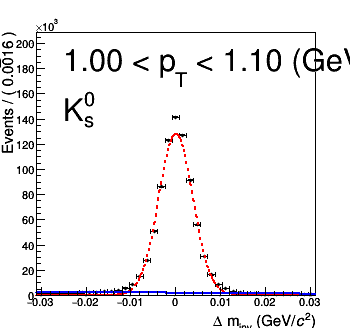
\includegraphics[width=.3\textwidth]{\imgpath/fitK0s.png}
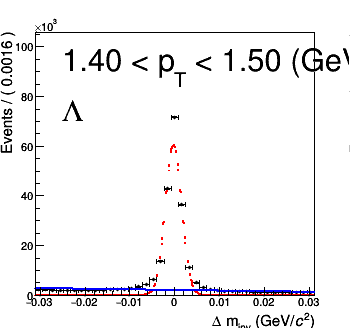
\includegraphics[width=.3\textwidth]{\imgpath/fitL.png}
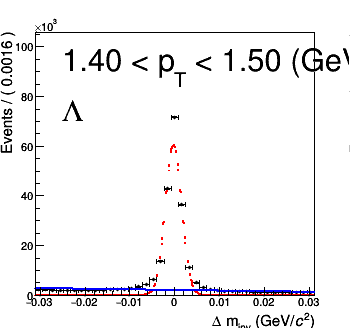
\includegraphics[width=.3\textwidth]{\imgpath/fitL.png}
\caption{Determination of the signal peak mean and width using a fit of the Gaussian distribution for \KOs, \LA, and \AL particles.}
\label{fig:analysis:peakfit}
\end{figure}

\begin{figure}
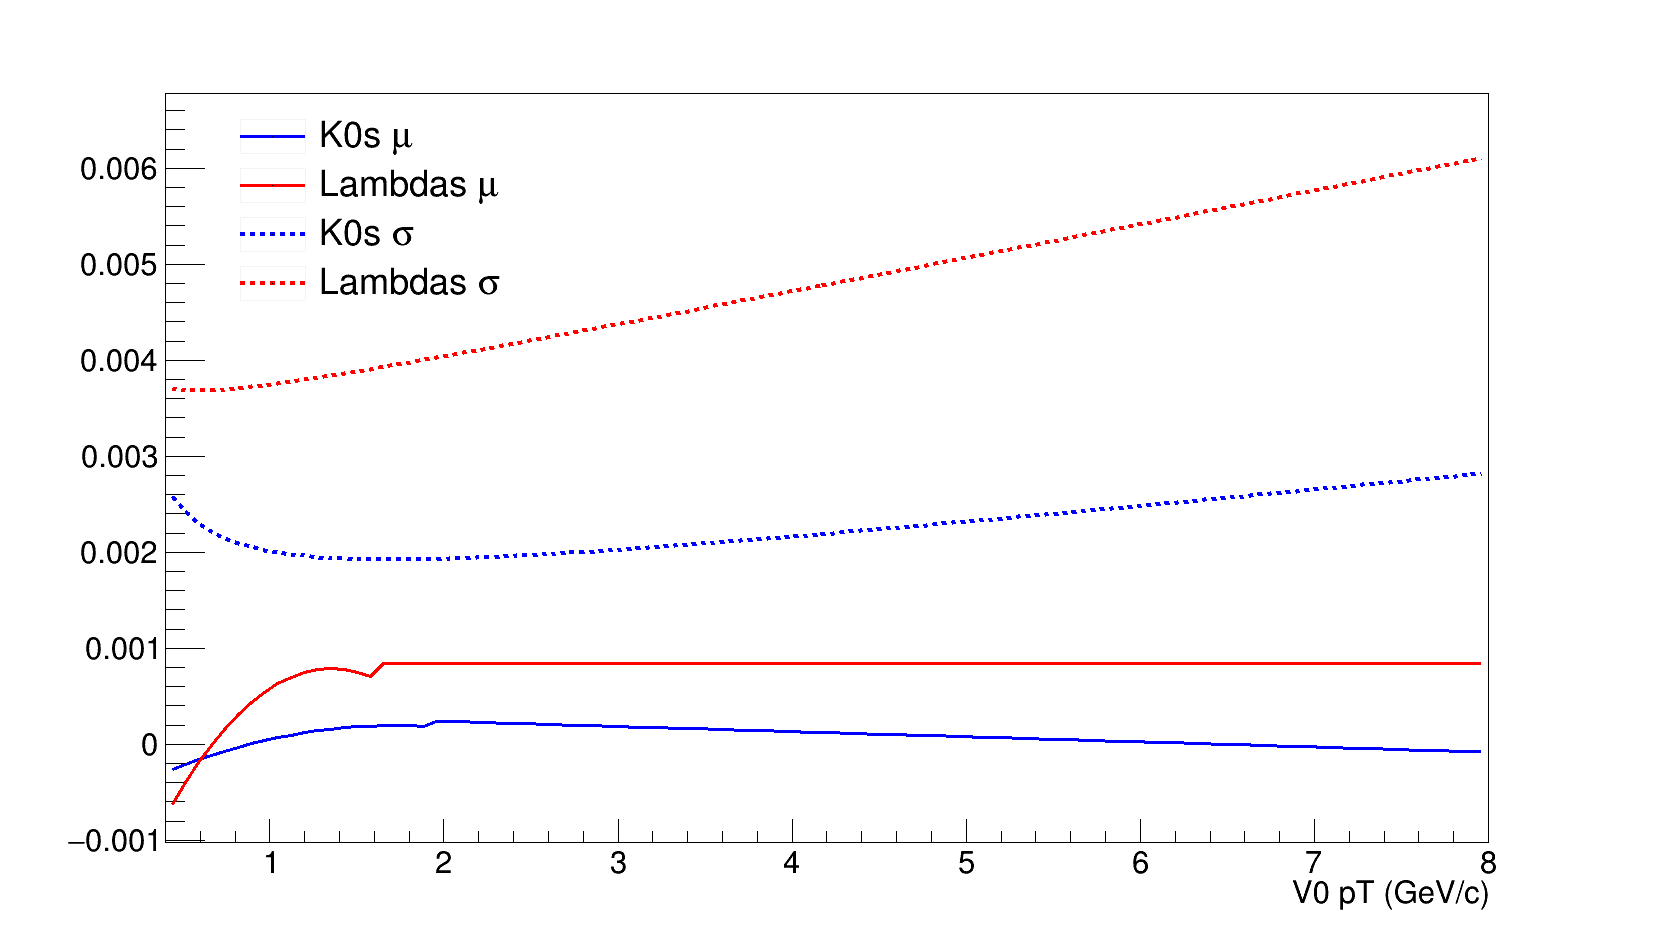
\includegraphics[width=.6\textwidth]{\imgpath/sidebands.png}
\caption{Parametrisation of the signal peak mean and width as a function of \pt.}
\label{fig:analysis:sigex}
\end{figure}


\begin{figure}
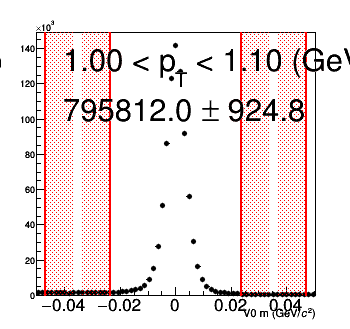
\includegraphics[width=.3\textwidth]{\imgpath/regionK0s.png}
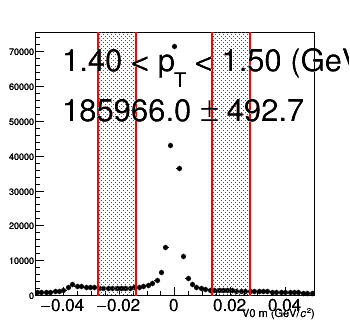
\includegraphics[width=.3\textwidth]{\imgpath/regionL.png}
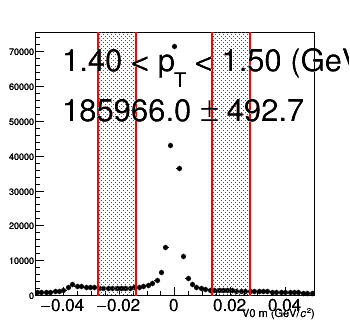
\includegraphics[width=.3\textwidth]{\imgpath/regionL.png}
\caption{Visualisation of the sideband regions, from which the background is estimated, for \KOs, \LA, and \AL particles.}
\label{fig:analysis:peakfit}
\end{figure}


\subsection{Validation using simulations}

The accuracy of the sideband method is tested with ``MC closure"---in MC simulated data, the \pt-spectra acquired blindly from the \VO candidates are compared with \pt-spectra of identified \VO. The ratios can be seen in Fig.~\ref{fig:analysis:sigexclosure} and show a $\sim5 \%$ effect at high-\pt. This is caused by the fact that in ALICE MC simulations, the \VO mass peaks have somewhat longer tails than in data and thus the signal can enter the background regions. This has to be taken into account when defining reconstruction efficiency using MC data.

\subsubsection*{Alternative approach}
Originally, methods involving a likelihood fit and an unbinned likelihood fit of two Gaussian distributions as well as other background descriptions were tested. However, although more sophisticated, these methods proved considerably less precise. This is due to the fact that the signal peaks cannot be accurately described by the two Gaussian distributions, particularly in highly populated \pt bins. That said, they are sufficient to determine the $\sigma_{\VO}$ for above-stated purposes.

\subsubsection*{Mass resolution of secondary \LA and \AL particles}
Approximately 20\% of the \LA yields measured are produced as secondary particles coming from decays of the \XI baryon in most cases -- also called feeddown. Investigations of the simulated data revealed that the invariant mass of these secondaries suffers from a worse resolution (ca.\ 3 times higher $\sigma$). Subsequently, this gives our signal extraction a ca. $75\%$ efficiency for secondaries, and ca. $95\%$ efficiency for inclusive \LA yields at intermediate \pt. This has to be taken into consideration when calculating corrections for the feeddown yields. This effect can be seen in Fig.~\ref{fig:analysis:masssecond}.

\begin{figure}%
\subfloat[][]{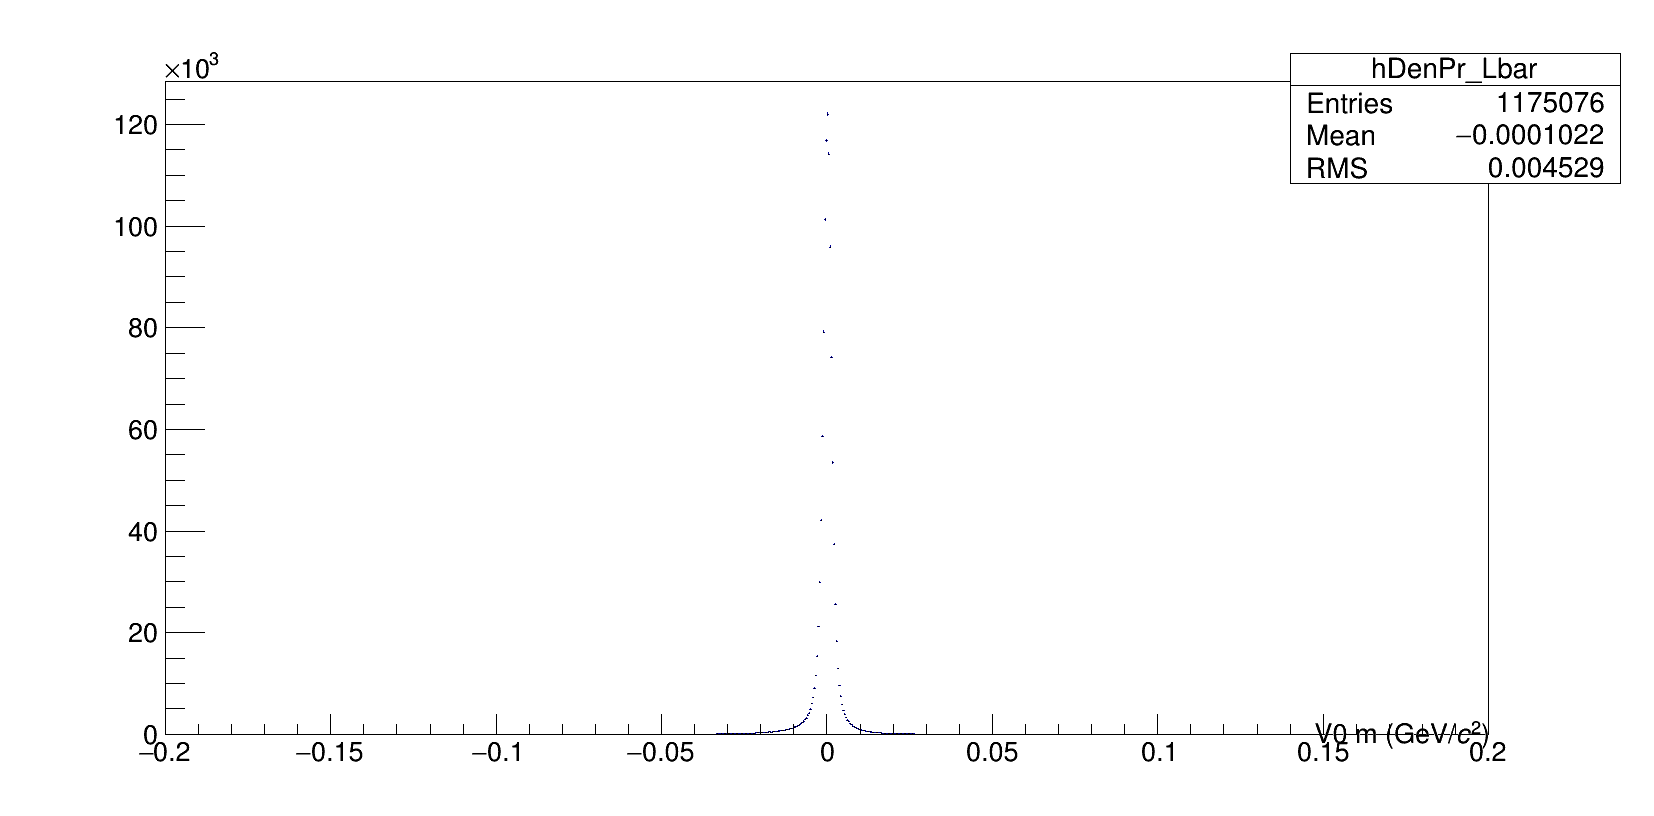
\includegraphics[width=.48\textwidth]{\imgpath/im_primaryPDG.png}}%
\subfloat[][]{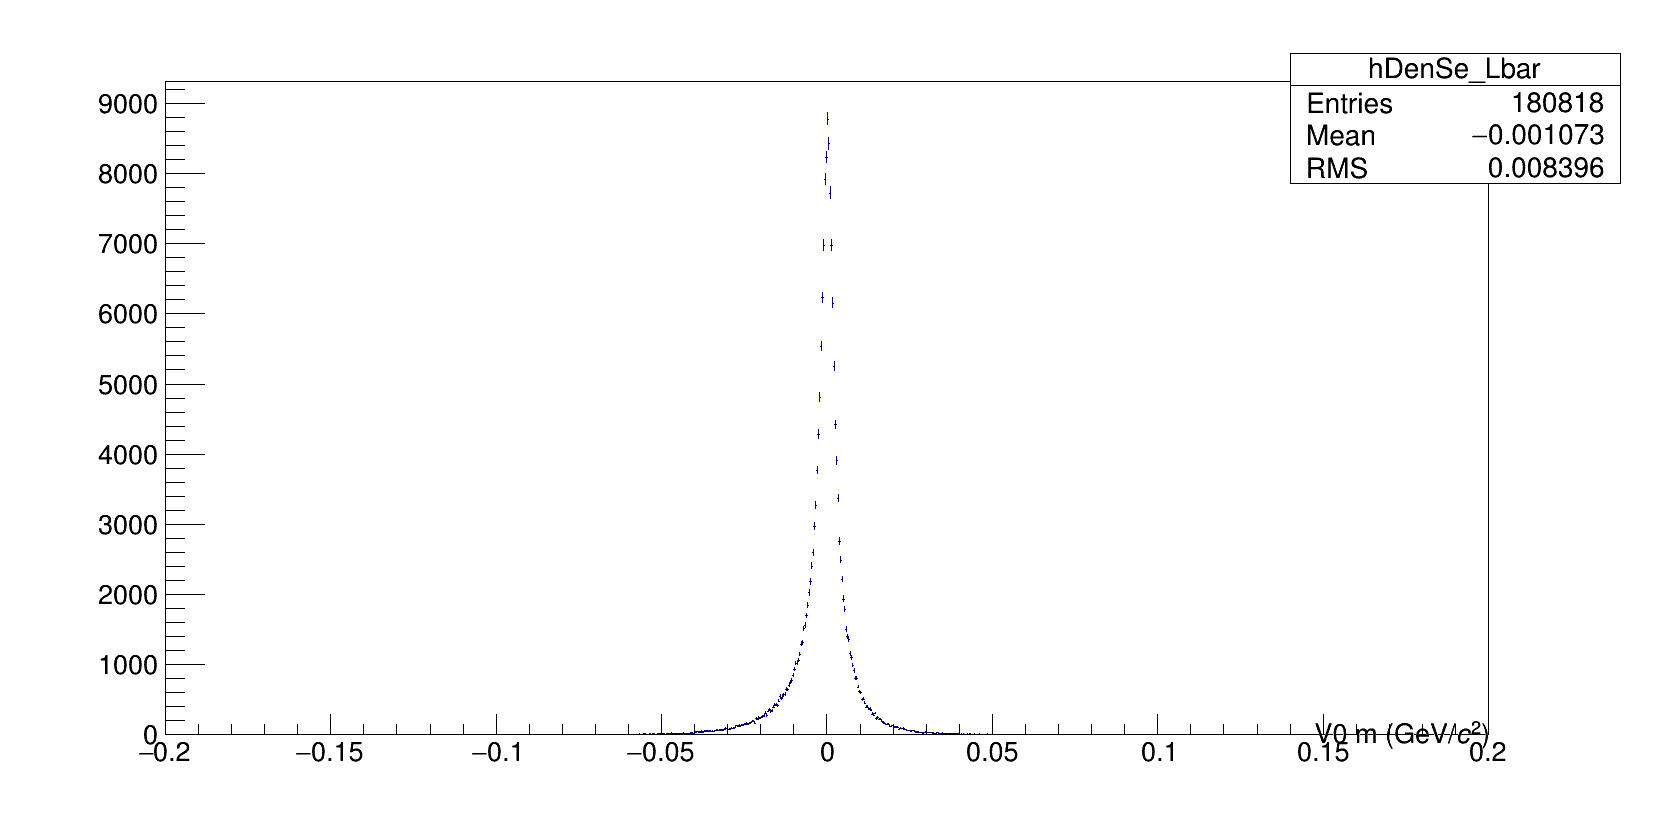
\includegraphics[width=.48\textwidth]{\imgpath/im_secondaryPDG.png}}%
\caption{TBA.}%
\label{fig:analysis:masssecond}%
\end{figure}

\section{Normalisation}

The reconstructed \KOs, \LA, and \AL yields $Y(\eta,\pt)$ are normalised according to

\begin{align}
\frac{\mathrm{d}^2 N^\mathrm{raw}}{\mathrm{d}y \mathrm{d}\pt} = \frac{1}{N_\mathrm{ev}} \frac{1}{J} \frac{1}{\Delta \eta} \frac{1}{\Delta \pt} Y(\eta,\pt) \quad ,
\end{align}
where $N_\mathrm{ev}$ is the number of selected events, $J$ the Jacobian of the $\eta \rightarrow y$ transformation, and $\Delta \eta$ and $\Delta \pt$ the widths of the pseudorapidity and transverse momentum intervals, respectively.

TBA Jacobian

TBA Event loss correction

\section{Corrections to the reconstructed production}

To acquire results with scientific relevance, the raw yields of \VOs observed with ALICE need to be corrected for geometrical acceptance, detector effects, and, in the case of \LA(\AL), also for secondary contribution.

\subsection{Secondary contribution correction}

Only ca.\ $80\%$ of the measured inclusive \LA and \AL yields are produced directly in the pp collision or near-instantanously in non-weak decays of resonances, as primary particles. The remainder is produced secondarily, as products of weak decays of heavier baryons. The dominant, and the only relevant, reactions are:
\begin{align}
\XI^- &\rightarrow \LA \, \pim \, \, , \\
\XI^0 &\rightarrow \LA \, \pi^0 \, \, ,\\
\XI^+ &\rightarrow \AL \, \pip \, \, ,\\
\overline{\XI}^0 &\rightarrow \AL \, \pi^0 \, \, .
\end{align}

For the \KOs, the secondary production (such as from $\phi$ mesons) is negligible.

The primary \LA yields can be estimated using the following equation,
\begin{align}
\LA^\mathrm{raw}_\mathrm{
} (\pt^i ) &= \LA^\mathrm{raw}_\mathrm{measured} - \LA^\mathrm{raw}_\mathrm{secondary}  \, \, \\
&= \LA^\mathrm{raw}_\mathrm{measured} - \sum_j F_{ij}^\LA \int_{\pt^j} \odv{N}{\pt} (\XI^-) \quad ,
\end{align}
where $F_{ij}$ is the so-called feeddown matrix giving the probabilities of a produced $\XI^-$ or $\XI^0$ particle in a \pt interval $j$ decaying into reconstructed \LA in a \pt interval $i$, and $\odv{N}{\pt} (\XI^-)$ the measured $\XI^-$ spectra.  This approach assumes that the $\XI^0$ decay contribution is identical to $\XI^-$ and is used because $\XI^0$ baryons are challenging to measure. For the \AL , the equation is analogous but uses $\XI^+$ .

The feeddown matrix is calculated in ALICE MC simulations of MB events,
\begin{align}
F_{ij}^\LA &= 2 \, \cdot \, \frac{N_\mathrm{rec.} (\LA) |_{\pt^\LA = i}^{\pt^{\XI} = j}}{N_\mathrm{gen.} (\XI) |_{\pt^{\XI} = j}} \quad ,
\end{align}
where \XI represent both $\XI^-$ and $\XI^0$. There is an assumption that the probabilities, and thus, the matrix, do not depend on multiplicity of the event. It is taken into account in systematic uncertainties.

An alternative approach is constructing $F_{ij}^\LA$ from charged \XI solely, and then multiplying $\LA^\mathrm{raw}_\mathrm{secondary}$ by two and was used to determine the systematic uncertainty.

As discussed previously, due to the worse mass resolution of secondary \LA, a \Minv cut of $5\sigma_{\VO}$ (determined in the sideband definition procedure). Since a large amount of the secondaries enter the background regions, a negative weight $-1$ has to be applied to achieve the best MC closure validation. Other configurations ($6\sigma_{\VO}$ and $-1$ weight, $4\sigma_{\VO}$ and $0$ weight) were also tested.

The feeddown matrices $F_{ij}^{\LA}$, $F_{ij}^{\AL}$ are displayed in Fig.~\ref{fig:analysis:fdmatrix}.

\begin{figure}%
\subfloat[][]{\includegraphics[width=.48\textwidth]{\imgpath/lbar_fdm.png}}%
\subfloat[][]{\includegraphics[width=.48\textwidth]{\imgpath/lbar_fdm.png}}%
\caption{Feeddown matrices \textbf{(a)} $F_{ij}^{\LA}$ and \textbf{(b)} $F_{ij}^{\AL}$ from \XI baryons.}%
\label{fig:analysis:fdmatrix}%
\end{figure}

\begin{figure}%
\includegraphics[width=.48\textwidth]{\imgpath/l_fd_hm.png}%
\caption{TBA.}%
\label{fig:analysis:fdfraction}%
\end{figure}

\subsubsection*{\XI spectra}

Fitting. TBA

\subsection{Reconstruction efficiency}

The total reconstruction efficiency, including the acceptance, for \VOs in our events with ALICE can be determined using the Monte Carlo simulated data. It is calculated as
\begin{align}
\epsilon ( \pt ) &= \mathrm{acceptance} \times \epsilon_\mathrm{rec}  \\
&=  \frac{\mathrm{\# \, associated \, reconstructed \, \VOs  }}{\mathrm{\# \, generated \, \VOs \, within \, |\eta|<0.8}}\, \, ,
\end{align}
in events that passed the selection criteria. The association is done by comparing the mother's and daughters' PDG ID as well as the MC generator label. Particles in the numerator have to satisfy all selection cuts. The reconstruction efficiency for \KOs, \LA, and \AL is plotted in Fig.~\ref{fig:analysis:effi}.

As mentioned before, in ALICE simulations, the \Minv resolution worsens with increasing \pt; in high-\pt bins, the simulated \VOs are sometimes reconstructed with higher \Minv than what is considered realistic. This would lead to a lower efficiency as those \VOs can fall out of the signal region, and an overestimation of the total measured spectra. For this reason, a $4\sigma_{\VO}$ cut is required for the \VOs \Minv in the numerator. Alternatively, one could use a cut of $6 \sigma_{\VO}$  and applying a negative weight $-1$ in cases where it is not satisfied. 

The reconstruction efficiency is defined in MB events, assuming the reconstruction in pp collisions does not largely depend on multiplicity, geometrical event classification, or event sub-structure. This assumption is taken into account in systematic uncertainties.

\begin{figure}%
\includegraphics[width=.95\textwidth]{\imgpath/cEffi.pdf}%
\caption{TBA.}%
\label{fig:analysis:effi}%
\end{figure}

\section{Transverse momentum spectra}

Using the corrections on the normalised yields, one acquires the measured transverse momentum spectra, which are comparable with production cross sections and thus theoretical predictions.

\begin{align}
\frac{\mathrm{d}^2 N}{\mathrm{d}y \mathrm{d}\pt} &= \epsilon (\pt) \times \frac{\mathrm{d}^2 N^\mathrm{raw}_\mathrm{primary}}{\mathrm{d}y \mathrm{d}\pt}
\end{align}

\subsection{Comparisons with previously published results}

The acquired results were tested against previously published measurements of \KOs, \LA, and \AL transverse momentum spectra at the ALICE experiment in MB as well as high-multiplicity (\VOM I and \VOM III) events in pp collisions at $\sqrt{s} = 13$~TeV.

\begin{figure}%
%\centering
\subfloat[][]{\includegraphics[width=.48\textwidth]{\imgpath/K0toK0_MBandV0M_offi}}%
\subfloat[][]{\includegraphics[width=.48\textwidth]{\imgpath/LtoL_MBandV0M_offi.png}}
\caption{Cross-checks of this analysis' \pt spectra of \textbf{(a)} \KOs and \textbf{(b)} \LA + \AL in MB, \VOM I, and \VOM I-III events in pp collisions at against $\sqrt{s} = 13$~TeV results previously published by ALICE.}%
\label{fig:analysis:xcheck}%
\end{figure}

\subsubsection*{\KOs}

The published \KOs results were measured in \spverb|kINT7| events. \cite{} Thus, in order to compare on an equal footing, a trigger efficiency scaling factor $\epsilon_\mathrm{trig} = 0.7448$, taken over from \cite{}, was applied to this analysis.

The comparison of this analysis to the published results can be seen in Fig.~\ref{fig:analysis:xcheck}a. In high-multiplicity events, the spectra are in a good agreement across the entire \pt range (most points lie within $\sim 5\%$ difference). In MB events, there is a difference ($\sim 10 \%$) at the lowest \pt values. This is understood as a loss of signal in events with no reconstructed charged tracks and is usually corrected for. Since the correction plays a role only in MB -- events which are of little interest to this thesis' work -- it is not taken into account.

\subsubsection*{\LA + \AL}

The published \LA + \AL results were measured in same events as this analysis, (\spverb|INEL>0|), therefore, $\epsilon_\mathrm{trig}$ was not applied. \cite{} They are compared to this analysis in Fig.~\ref{fig:analysis:xcheck}b and show a satisfactory agreement (most points lie within $\sim 5\%$ difference).

\section{Systematic uncertainties}

Experimentally measured values always come with uncertainties -- statistical and systematic. Whereas statistical uncertainties are caused by the limited number of measurements and can be decreased by increasing the statistical sample analyzed, systematic uncertainties represent the imprecision or the bias of the experimental methodology itself. Calculation of statistical uncertainties is given directly from frequentist statistics. Definition of systematic uncertanties, however, is not always straightforward -- one cannot simply re-do the measurement with several completely different experimental setups and data analysis techniques. Therefore, a lot of effort needs to go into identifying all possible sources of systematic uncertainties.

In this measurement, the following sources of systematic uncertainty were identified as relevant:
\begin{itemize}
\item \textbf{Variation of selection criteria}\\
In determining the reconstruction efficiency, it is assumed that in ALICE MC simulations, all observables used for the identification of \VOs and for assuring the quality of daughter tracks represent reality. Their inaccurate description, however, results in a bias. This bias is estimated by testing the sensitivity of the final results to varying the selection criteria on these observables.
\item \textbf{Signal extraction method}\\
The biases of the sideband background estimation procedure are tested against increasing and reducing the signal and background regions, by varying the number of $\sigma_{\VO}$. Variations of $5$ and $7 \, \sigma_{\VO}$ were used.
\item \textbf{Multiplicity dependence of $\epsilon ( \pt )$}\\
Studies of the reconstruction efficiency in pp collisions reveal a small, albeit significant dependence on the collision final state. A constant uncertainty of $\sim 2 \%$ is applied on the spectra to account for this.
\item \textbf{Feeddown correction}\\ 
Three sources of uncertainty on the contribution of secondary particles were identified -- variation of the \XI yields, multiplicity dependence of the feeddown matrix, and an alternative method.% First, the \XI yields, from which the feeddown is calculated, are varied within their reported uncertainties. Second, similarily to $\epsilon ( \pt )$, the assumption of no multiplicity dependence of the feeddown matrix is accompanied by a constant uncertainty of $2 \%$ on the secondary yields. Lastly, an alternative method of estimating the feeddown just from charged \XI baryons, and multiplying by a factor of two revealed a systematic uncertainty
\item \textbf{Material budget}\\
This uncertainty reflects that implementing ALICE's material composition in simulations comes with limitations. Previous studies in ALICE \cite{} which varied parameters of the description of the apparatus showed that this effect corresponds to a constant $4\%$ uncertainty on the measured spectra.
\end{itemize}

When testing the default method $A$ against an alternative method $B$, one can implement the deviation of the ratio of their measured values $\Delta = B / A$ from unity as an uncertainty. To ensure that this difference is statistically significant and not just an effect of a limited data sample, the deviation is considered only if it exceeds its own uncertainty, defined as
\begin{align}
\sigma_\Delta = \frac{\sqrt{|\sigma_B^2 - \sigma_A^2|}}{A} \quad ,
\end{align}
where $\sigma_A$ and $\sigma_B$ are the uncertainties of the results from methods $A$ and $B$, respectively.

\subsection{Variation of selection criteria}

To investigate the differences between description of variables in measured data and ALICE simulations, and determine sensible cut variations $\lambda_i$, raw yield loss $F$ was studied. It was measured in MB events and defined as
\begin{align}
F(\lambda) = 1 - \frac{Y(\lambda)}{Y(\lambda_0)} \quad ,
\end{align}
where $Y(\lambda)$ is the raw yield as a function of the cut value $\lambda$ and $\lambda_\mathrm{LOOSEST}$ the loosest variation (corresponding to the highest yield). 

For most observables, the systematic effect can be estimated from alternative methods using $\lambda_\mathrm{LOOSEST}$ and $\lambda_\mathrm{TIGHTEST}$. To ensure the stability and possible non-linearity, less strict $\lambda_\mathrm{LOOSE}$ and $\lambda_\mathrm{TIGHT}$ are also tested. If applicable t is reasonable to choose $\lambda_i$ such that $F(\lambda_i)$ does not exceed approximately $10\%$.

The $F(\lambda)$ for the different selection critera, and with the chosen $\lambda_i$ are shown in Fig.~\ref{fig:analysis:rylK0s}, Fig.~\ref{fig:analysis:rylL}, and Fig.~\ref{fig:analysis:rylAL} for \KOs, \LA, and \AL, respectively. The pile-up rejection cut, which requires ``fast detector" information for at least one daughter is of a binary nature. So, its variation was tested by requiring a different amount of ``fast detector" hits between the two daughters. The selected values of $\lambda_i$ are summarised in Tab.~\ref{tab:analysis:cutvariations}.

\begin{figure}
\includegraphics[width=.95\textwidth]{\imgpath/cRYL_K0s.png}
\caption{TBA}
\label{fig:analysis:rylK0s}
\end{figure}

\begin{figure}
\includegraphics[width=.95\textwidth]{\imgpath/cRYL_L.png}
\caption{TBA}
\label{fig:analysis:rylL}
\end{figure}

\begin{figure}
\includegraphics[width=.95\textwidth]{\imgpath/cRYL_Lbar.png}
\caption{TBA}
\label{fig:analysis:rylAL}
\end{figure}

\begin{table}[h!]
\begin{center}
\begin{tabular}{|c|c|c|c|c|c|}
\hline
 \bf Quality & \bf loosest & \bf loose & \bf default & \bf tight & \bf tightest \\ \hline
radius & 0.3 & 0.4 & 0.5 & 0.6 & 0.7 \\ \hline
DCA between daughters & 1.5 & 1.25 & 1.0 & 0.75 & 0.5 \\ \hline
cos PA & 0.95 (0.993) & 0.96 (0.994) & 0.97 (0.995) & 0.98 (0.996) & 0.99 (0.997) \\ \hline
pile-up removal cut & - & - & 1 & 2 & - \\ \hline
comp.\ mass number of $\sigma$ & 2.5 & 3.0 & 4.0 & 5.0 & 5.5 \\ \hline
lifetime & - & (35.0) & (30.0) & (25.0) & - \\ \hline
TPC PID number of $\sigma$ & 6.5 & 6.0 & 5.0 & 4.0 & 3.5 \\ \hline
DCA to PV of pos.\ track & 0.05 & 0.055 & 0.06 & 0.07 & 0.08 \\ \hline
DCA to PV of neg.\ track & 0.05 & 0.055 & 0.06 & 0.07 & 0.08 \\ \hline
TPC crossed rows & - & - & 70 & 75 & 80 \\ \hline
TPC find.\ ratio & - & - & 0.8 & 0.95 & - \\ \hline
\end{tabular}
\end{center}
\caption{Cut variation parameters for the \KOs (\LA and \AL).}
\label{tab:analysis:cutvariations}
\end{table}

\subsection{Feeddown correction}

As mention before, first, the \XI spectra, from which the feeddown is calculated, are varied within their reported uncertainties. In both variations, the yields are then extracted using a fit.  Second, similarily to $\epsilon ( \pt )$, the assumption of no multiplicity dependence of the feeddown matrix is accompanied by a constant uncertainty of $2 \%$ on the secondary yields (corresponding to ca.\ $0.6\%$ uncertainty on the primary yields). %WRONG ACTUALLY

Lastly, an alternative method of estimating the feeddown just from charged \XI baryons, and multiplying by a factor of two, was also tested and contributes a systematic uncertainty. It is considered significant and applied when $|\Delta - 1| > \sigma_\Delta$. The difference between the two methods can be seen in Fig.~\ref{fig:analysis:fdmethod}. It should be noted that whilst the secondary yields suffer from a rather large systematic uncertainty, the effect on the primary spectra is significantly smaller, as the uncertainties enter as $\frac{1-B}{1-A}$ and the secondary yields do not exceed $\sim 30\%$.

\begin{figure}
\includegraphics[width=.65\textwidth]{\imgpath/L_fd_mb.png}
\caption{TBA}
\label{fig:analysis:fdmethod}
\end{figure}



\chapter{Transverse Spherocity}
\def \imgpath {"./figures/sphero"}
In this chapter, measurements of \KOs, \LA, and \AL are reported as a function of transverse spherocity \SOPT, a measure of the event's topology in the transverse $xy-$plane. 
\section{Transverse spherocity}

\subsection{Motivation for studying event topology}

As explained in Chapter X, there is overwhelming evidence that some phenomena associated with QGP, such as collective flow and strangeness enhancement, also arise in pp and p--A collisions at LHC energies and high event multiplicities. This challenges the conventional assumption that the hadron densities and densities of colour fields between partons are too low to interact with each other. Consequently, high-multiplicity pp (and p--A) collisions cannot be treated as a superposition of mostly independent parton-parton (or parton-hadron) scatterings and a more in-depth approach  is required to fully understand these phenomena.

Event shape observables have been used historically in lepton experiments to study fundamental QCD properties such as the gluon spin \cite{petra-tasso-gluonspin}, and also at Tevatron and the LHC in events with very high \pt ($\gtrsim 100~\gevc$) jets to further test pQCD predictions \cite{antonio-sphero-motivation}. There are various observables, including sphericity, spherocity, thrust, F-parameter, and Ellis-Karliner angle, most of which are collinear- and infrared-safe and therefore moderately easily calculable\cite{banfi-eventshape-pheno}. An illustration of two events with different topologies and calculated values of selected observables can be seen in Fig.~\ref{fig:sphero:topologies}.

\begin{figure}%
\includegraphics[width=.90\textwidth]{\imgpath/event-observables.png}
\caption{TBA.}
\label{fig:sphero:topologies}
\end{figure}

With the discoveries of QGP phenomena in high-multiplicity collisions of small systems, event shape observables become attractive for different reasons. This is because pQCD (``hard") processes are responsible for a significant fraction of particle production and are likely to impact the character of QGP phenomena in non-trivial ways. The role of non-perturbative (``soft") processes is particularly interesting to study as their mechanisms are not fully understood and their interpretation relies on phenomenological models that require clear experimental measurements with high discriminatory power. 

Event shape observables allow us to quantify events according to the dominant contributing processes. For instance, collisions with single large \pt transfer scatterings are likely to lead into events with two back-to-back, highly collimated showers, which create a pencil-like shape in the transverse plane. Conversely, collisions with multiple lower \pt transfer partonic interactions will exhibit a high degree of azimuthal isotropy. Therefore, event shape measurements help us gain a deeper understanding of high-multiplicity events and a better control over the magnitudes of the hard and soft contributions. Ultimately, these measurements may help determine whether QGP formation is necessary in small systems or uncover new physical behaviours.

\subsection{\SO and \SOPT as experimental observables}

Traditionally, spherocity \SO is defined as:

\begin{align}
\SO = \frac{\pi^2}{4} \min_{\hat{n}} \left(\frac{\sum_i
      |p_{\textrm{T},i} \times \hat{n}|}{\sum_i
      |p_{\textrm{T},i}|}  \right)^2 \quad ,
\end{align}
where $p_{\textrm{T},i}$ represents the vector of transverse momentum of a particle $i$ and $\hat{n}$ is the event-dependent unit vector that minimises the sum. The sum runs over all charged particles in the event within the detector acceptance.

Previous ALICE measurements \cite{alice-spherocity} studied characteristics of charged particles in pp collisions and discovered their strong dependence of \meanpt on spherocity \SO, which validates the previously discussed motivation. This relationship is shown in Fig.~\ref{fig:sphero:nchpt}. Additionally, phenomenological studies of \SO in Pythia 8 further demonstrate its classifying power by finding strong dependence of \meannmpi as well as the mean number of reconstructed jets $\langle n_\mathrm{j} \rangle$ on \SO\cite{antonio-sphero-mpi}\cite{antonio-sphero-njets}. These results can be seen in Fig.~\ref{fig:sphero:nmpinjets}.

\begin{figure}%
\includegraphics[width=.60\textwidth]{\imgpath/alice_sphero_meanpt.pdf}
\caption{TBA.}
\label{fig:sphero:nchpt}
\end{figure}

\begin{figure}%
\subfloat[][]{\includegraphics[width=.48\textwidth]{\imgpath/sphero_nmpi.png}}
\subfloat[][]{\includegraphics[width=.48\textwidth]{\imgpath/sphero_njets.png}}\\
\caption{TBA.}
\label{fig:sphero:nmpinjets}
\end{figure}

This work uses a modified definition of this observable, \textit{unweighted} transverse spherocity \SOPT, defined as follows:

\begin{align}
\SOPT = \frac{\pi^2}{4} \min_{\hat{n}} \left(\frac{\sum_i
      |\hat{p}_{\textrm{T},i} \times \hat{n}|}{N_{\textrm{trks}}}  \right)^2 \quad ,
\label{eq:sOpt}      
\end{align}
where $\hat{p_{\textrm{T},i}}$ represents the \textit{unit} vector of transverse momentum of a particle $i$ and $N_{\textrm{trks}}$ the number of charged particles entering the sum. 

In this thesis, unless stated otherwise, the terms transverse spherocity and spherocity are both used to refer to this unweighted transverse spherocity \SOPT.

Applying the spherocity \SOPT, events in two geometrical limits can be studied:
\begin{itemize}
\item $\SOPT \rightarrow 0$ : the \textbf{``jetty"} limit. Pencil-like topology is selected. These events are dominated by hard pQCD processes. In this limit, with perfectly collimated back-to-back particles, $\hat{n}$ coincides with them. Thus, the sum of vector products in Eq.~\ref{eq:sOpt} contains only zero values as $\sin 0 = \sin \pi = 0$.
\item $\SOPT \rightarrow 1$ : the \textbf{``isotropic"} limit. Circular topology is selected. Such events are dominated by multiple softer non-perturbative processes\footnote{However, it is important to mention that  anisotropic collective flow such as $v_2$, a non-perturbative phenomenon, reduces the event isotropy.}. In this limit of $N\rightarrow\infty$ uniformly distributed unit vectors within $(0,2\pi)$, the choice of $\hat{n}$ becomes arbitrary and calculation of the sum in Eq.~\ref{eq:sOpt} leads to:
 \begin{align}
\frac{1}{N} \sum_{n=1}^N | \sin\frac{2\pi n}{N}| &\approx \frac{1}{N} \int_0^N |\sin\frac{2\pi x}{N}| \mathrm{d}x \\ 
&= \frac{2}{N} \int_0^{N/2} \sin\frac{2\pi x}{N} \mathrm{d}x = \frac{1}{\pi} \int_0^{\pi} \sin u \mathrm{d}u \\
&= \frac{1}{\pi} \left[-\cos x\right]_0^{\pi} = \frac{2}{\pi} \quad \,
\end{align}
and therefore $\SOPT=1$. 
\end{itemize}

Figure~\ref{fig:sphero:shapelimits} illustrates how spherocity slowly approaches the circular limit value with increasing $N$ compared to other event shape observables. This property makes spherocity favoured by experimentalists in these measurements, as it provides the highest discrimination power of isotropic events \cite{antonio-sphero-motivation}.

\begin{figure}%
\includegraphics[width=.90\textwidth]{\imgpath/sphero-shapelimits.png}
\caption{TBA.}
\label{fig:sphero:shapelimits}
\end{figure}


\subsection{Relationship between \SOPT and \SO}

In ALICE, only charged particles are considered when calculating spherocities. This introduces biases when measuring charged and neutral species of hadrons. For instance, even topologically identical events with dominant high-\pt leading $\pi^+$ and $\pi^0$ can yield significantly different values of the traditional \pt-weighted spherocity \SO, despite being comparable in all relevant aspects. In contrast, unweighted spherocity \SOPT offers a more similar quantification of the two events, as shown in Fig.~\ref{fig:sphero:sOvssOpt}. However, it should be noted that this modified definition is only applicable to events with many tracks (i.e., $N_{\textrm{trks}}>10$).

\begin{figure}%
\includegraphics[width=.70\textwidth]{\imgpath/SOvsSOPT2_up.png}
\caption{TBA.}
\label{fig:sphero:sOvssOpt}
\end{figure}

In addition, while not a large concern in high-multiplicity collisions\cite{alice-sphero-nch}, \SOPT also offers improved resolution compared to \SO, as the failure to reconstruct a high-\pt track has a smaller impact. Overall, \SO and \SOPT exhibit similar values and interpretations, with a strong correlation between the two, as illustrated in Fig.~\ref{fig:sphero:sOvssOptcorr}.

\begin{figure}%
%\includegraphics[width=.70\textwidth]{\imgpath/SOvsSOPT2_up.png}
\includegraphics[width=.70\textwidth]{example-image-a}
\caption{TBA.}
\label{fig:sphero:sOvssOptcorr}
\end{figure}

\subsection{Track and event selection}\label{sec:sphero:eventtracks}

The measurements are carried out on MB events with \INELgtO, requiring at least one hit in the \VOA or \VOC scintillators and one charged particle reconstructed within $|\eta|<1$. The primary vertex is reconstructed using hits in the SPD and is required to be within $10$~cm of the interaction point. The fast read-out time of the SPD allows rejection of out-of-bunch pile-up. In-bunch pile-up is further removed by excluding events with multiple reconstructed vertices. The presented results are based on high-multiplicity events, selected by the classifiers \VOM (forward rapidity) and \tracklet (mid-rapidity), and require a minimum of 10 reconstructed tracks within $|\eta|<0.8$ and with $\pt>\gevc{0.15}$.

To ensure a high level of azimuthal acceptance uniformity, which is important for event shape measurements, the following, rather loose, selection criteria are employed:
\begin{enumerate}
\item The SPD is not used due to its holes, at the expense of a lower momentum resolution.
\item A track is required to have at least 50 clusters in the TPC and be matched to hits in the ITS to improve tracking precision and further reject  pile-up.
\item DCA cuts are applied in both the longitudinal ($|\mathrm{DCA}_z|<3.2$~cm) and transverse ($|\mathrm{DCA}_{xy}|<2.4$~cm) planes to ensure that the reconstructed TPC track points to the primary vertex.
\end{enumerate}
It should be noted that charged decay products of \VOs with low \pt ($\lesssim \gevc{1}$) and small decay radius may enter and influence \SOPT determination.

\subsection{Multiplicity selection and its interplay with \SOPT}

Spherocity exhibits a twofold correlation with multiplicity that is not particularly informative. First, the definition of \SOPT results in higher values for events with more uniformly distributed particles, as shown in Fig.~\ref{fig:sphero:shapelimits}. Second, in models such as Pythia, high multiplicity is often associated with more MPI, which tend to lead to higher isotropy due to the increased number of emission sources. To gain a more nuanced understanding of the relationship between spherocity and multiplicity, we analyze the effect of \SOPT on measured particles in high-multiplicity events determined in two distinct rapidity regions, as described above. Specifically, the top $1\%$ ($10\%$) quantiles are used, denoted as \VOM I and \NSPD I (\VOM I-III and \NSPD I-III).

Figure~\ref{fig:sphero:v0mvscl1} shows the effect of \SOPT on the pion yields and \meanpt. Pions are measured in the high-multiplicity events and in top and bottom $10\%$ and $1\%$ quantiles of \SOPT. The result reveals that when measuring multiplicity in forward rapidity (\VOM I), the effect of \SOPT causes a change of approximately $100\%$ in the yields when going from jetty to isotropic limits, whereas the difference in \meanpt is only ca.\ $10\%$. Conversely, when determining the multiplicity in mid-rapidity (\NSPD I), the same region where the pion spectra are reconstructed, the change in the yields is only approximately $10\%$ while the change in \meanpt is ca.\ $25\%$.

For this reason, the following combinations of multiplicity and \SOPT selections are presented:
\begin{enumerate}
\item \NSPD I and \SOPT top and bottom $10\%$ quantiles: This selection emphasises the impact of extreme event topologies on the QCD processes whilst minimising the effect of multiplicity dependence.
\item \NSPD I-III and \SOPT top and bottom $1\%$ quantiles: This selection shows the effect of even more extreme event topologies but with overall less and somewhat varying multiplicity. 
\item \VOM I and \SOPT top and bottom $10\%$ quantiles: This selection highlights the effect of extreme event topologies with highly varying mid-rapidity multiplicity. It also allows for a comparison with \NSPD I-III and \SOPT $1\%$ selection, as the mid-rapidity multiplicity and the \meanpt variations are more similar.
\end{enumerate}

\begin{figure}%
\includegraphics[width=.70\textwidth]{\imgpath/mgPion_0.pdf}
\caption{TBA.}
\label{fig:sphero:v0mvscl1}
\end{figure}

The mid-rapidity multiplicities in the different high-multiplicity classes are reported in Tab.~\ref{tab:sphero:hm}. The measured \SOPT distributions in \NSPD I, \NSPD I-III, and \VOM I-III are shown in Fig.~\ref{fig:sphero:sopt}. They are treated with Bayesian unfolding to account for reconstruction effects. They are also compared with theoretical predictions from Pythia 8 (Monash and Ropes tunes), EPOS LHC, and Herwig. Table~\ref{tab:sphero:sOpt} provides the \SOPT cut values associated with the quantile selections in data.

\begin{figure}[!htb]%
\subfloat[][]{\includegraphics[width=.60\textwidth]{\imgpath/SO_Unfolded_CL1_Perc_1.pdf}}\\
\subfloat[][]{\includegraphics[width=.60\textwidth]{\imgpath/SO_Unfolded_CL1_Perc_10.pdf}}\\
\subfloat[][]{\includegraphics[width=.60\textwidth]{\imgpath/SO_Unfolded_V0M_Perc_1.pdf}}\\
\caption{The measured and fully corrected \SOPT distributions for both \textbf{(a)} \NSPD 0--1\%, \textbf{(b)} 0--10\% and \textbf{(c)} \VOM 0--1\% . The curves represent different model prediction, where the shaded area represents the statistical uncertainty of the models.}
\label{fig:sphero:sopt}
\end{figure}

%ˇ\begin{table}[h]
%\centering
%\caption{TBA}
%\label{tab:sphero:hm}
%\begin{tabular}{|c|c|c|c|c|}
%\hline
%\textbf{Event class} & \textbf{\NSPD I} & \textbf{\NSPD I-III} & %\textbf{\VOM I} & \textbf{\VOM I-III} \ \hline
%$\avdndeta$ & $18.7 \pm 0.25$ & $21.57 \pm 0.32$ & $26.02 \pm 0.35$ & %$33.01 \pm 0.55$ \ \hline
%\end{tabular}
%\end{table}

\begin{table}[h!]
\centering
\caption{TBA.}
\label{tab:sphero:hm}

\begin{tabular}{|cc|ccc|}
\hline
\multicolumn{2}{|r|}{\parbox[b][1.2em]{2em}{} Event class} & \NSPD I & \NSPD I-III & \VOM I \\ \hline
%\multicolumn{2}{l|}{} & \multicolumn{3}{l}{} \\
%\multicolumn{5}{l}{\parbox[b][1.4em]{1em}{Jetty}} \\ \hline
\multicolumn{2}{|l|}{\parbox[b][1.1em]{1em}{}\avdndeta} & $33.01 \pm 0.55$ & $21.57\pm 0.32$ & $26.02 \pm 0.35$ \\ \hline
\end{tabular}
\end{table}

\begin{table}[h!]
\centering
\caption{Values of the different quantiles of the uncorrected \SOPT distribution used for the event selections in this analysis.}\label{tab:sphero:sopt}

\begin{tabular}{|cc|ccc|}
\hline
\multicolumn{2}{|r|}{\parbox[b][1.2em]{2em}{} Event class} & \NSPD I & \NSPD I-III & \VOM I \\ \hline
%\multicolumn{2}{l|}{} & \multicolumn{3}{l}{} \\
\multicolumn{5}{l}{\parbox[b][1.4em]{1em}{Jetty}} \\ \hline
\multicolumn{2}{|l|}{\parbox[b][1.1em]{1em}{}\SOPT 0--1\%} & $<0.487$ & $<0.408$ & $<0.433$ \\
\multicolumn{2}{|l|}{\SOPT 0--10\%} & $<0.624$ & $<0.561$ & $<0.589$ \\
\hline
\multicolumn{5}{l}{\parbox[b][1.2em]{1em}{Isotropic}} \\ \hline
\multicolumn{2}{|l|}{\SOPT 90--100\%} & $>0.892$ & $>0.871$ & $>0.882$ \\
\multicolumn{2}{|l|}{\SOPT 99--100\%} & $>0.942$ & $>0.930$ & $>0.936$ \\ \hline
\end{tabular}
\end{table}

\subsection{Comparison of \VO production with MC generators}

Further on in this chapter, the results of \KOs, \LA, and \AL as a function of \SOPT are presented and compared with predictions from phenomenological models Pythia 8, EPOS LHC, and Herwig obtained from MC simulations. To mitigate the effect of reconstruction on the experimental results and make the comparison with these predictions as comparable as possible, the following strategies were employed based on findings using the ALICE MC simulations:
\begin{itemize}
\item The results were compared using the same quantiles of the \SOPT distributions in both the MC and the data, instead of relying on the experimental \SOPT ranges determined by specific cut values. This approach reduced the effects of \SOPT resolution.
\item In the MC simulations, the \SOPT calculations included neutral particles \KOs, \LA, and \AL, despite their neutral charge. This helped minimize differences between the true and reconstructed/corrected MC results, possible due to the potential contribution of charged \VO daughters to the \SOPT calculation. 
\end{itemize}
Any discrepancies that still persisted between the true and reconstructed/corrected transverse momentum spectra were accounted for as systematic uncertainties.

\section{Systematic uncertainties}

The systematic uncertainties associated with the \pt spectra of \KOs, \LA, and \AL were evaluated separately for \NSPD I and \VOM I events with no \SOPT selection, as well as for the top and bottom $10\%$ isotropic and jetty quantiles, using the methodology described in Section~\ref{sec:ana:systematics}. The relative systematic uncertainties obtained from these configurations were also applied to the \NSPD I-III and \VOM I-III event classes with different jetty/isotropic quantiles.

\subsection{Variations in alternative methods}

Figures~\ref{fig:sphero:systK0s}, \ref{fig:sphero:systLA}, and \ref{fig:sphero:systAL} illustrate the variations resulting from alternative cut values, extraction parameters, or feeddown methods in \VOM I, \SOPT-unbiased events for \KOs, \LA, and \AL, respectively. The maximal deviations, contributing to the final systematic uncertainties, are also shown.

\begin{figure}[!h]
  \centering
\includegraphics[width=.98\textwidth]{\imgpath/cDev_K0s_V0M01_MB.png}
  \caption{Deviations of the corrected spectra w.r.t.\ the different cut variations used for the \Ks . The maximum deviation is added in quadrature to the total, if it's larger than $\sigma_\mathrm{RB}$ (depicted as errorbars) from unity.}
  \label{fig:sphero:systK0s}
\end{figure}

\begin{figure}[!h]
  \centering
\includegraphics[width=.98\textwidth]{\imgpath/cDev_L_V0M01_MB.png}
  \caption{Deviations of the corrected spectra w.r.t.\ the different cut variations used for the \Ks . The maximum deviation is added in quadrature to the total, if it's larger than $\sigma_\mathrm{RB}$ (depicted as errorbars) from unity.}
  \label{fig:sphero:systLA}
\end{figure}

\begin{figure}[!h]
  \centering
\includegraphics[width=.98\textwidth]{\imgpath/cDev_Lbar_V0M01_MB.png}
  \caption{Deviations of the corrected spectra w.r.t.\ the different cut variations used for the \Ks . The maximum deviation is added in quadrature to the total, if it's larger than $\sigma_\mathrm{RB}$ (depicted as errorbars) from unity.}
  \label{fig:sphero:systAL}
\end{figure}

\subsection{Experimental bias}

TBA

\subsection{Correlation of uncertainties with \SOPT}

Correlations of several systematic uncertainties with respect to the \SOPT selection are expected. Since the ratios of jetty/isotropic results to \SOPT-unbiased ones provide important insights, it is necessary to study and account for these correlations.

TBA add methodology.

The systematic uncertainty associated with the material budget is fully correlated, while assuming the reconstruction efficiency is independent of multiplicity leads to an uncorrelated uncertainty. This assumption would lead to a factor of $\sqrt{2}$ in the ratios of jetty/isotropic to \SOPT-unbiased for this uncertainty. However, in ALICE, this assumption is generally considered too conservative by ALICE, and thus this factor is dropped. The same approach is used for the uncertainty associated with the multiplicity independence of the feeddown matrix. Detailed results can be found in Appendix~\ref{app:spherosyst}.


\subsection{Summary}

The total systematic uncertainties are reported in Tab.~\ref{tab:sphero:syst} and visualised in Fig.~\ref{fig:sphero:systtot}.

\begin{figure}[!h]
\centering
\subfloat[][]{\includegraphics[height=.3\textheight]{\imgpath/k0s_sys.pdf}}\\
\subfloat[][]{\includegraphics[height=.3\textheight]{\imgpath/l_sys.pdf}}\\
\subfloat[][]{\includegraphics[height=.3\textheight]{\imgpath/lbar_sys.pdf}}\\
\caption{Total relative systematic uncertainty and individual contributions for the \KOs, \LA, and \AL .}
\label{fig:sphero:systtot}
\end{figure}

\begin{table}[h!]
\centering
\caption{The most relevant systematic uncertainties for the long-lived particles \KOs and \LA(\AL) as a function of \SOPT. ``HM'' in this table represents the \SOPT-unbiased spectra. Uncertainties are pt-dependent, and the ranges listed represents the minimum-maximum values presented in the final spectra (see text for details). }
\label{tab:sphero:syst}
\begin{tabular}{|l|lllll|}
\hline
\multicolumn{1}{|r|}{Topology:}              & Jetty     & Iso       & HM        & Jetty/HM       & Iso/HM      \\ \hline

\multicolumn{6}{l}{\parbox[b][1.2em]{1em}{K$^0_\mathrm{S}$}} \\
\hline
Selection cuts        & 3\%    & 3--4\%     & 3--4\%     & Negl.          & 1\%          \\
Track pile--up        & 1\% & 1--3\% & 1\% & 0--2\% & 0--2\%   \\
Signal extraction     & 1--3\%     & 1--3\%     & 1--3\%     & Negl. & Negl. \\
Efficiency            & 2\%    & 2\%    & 2\%    & 2\%         & 2\%         \\
Material budget       & 4\%    & 4\%    & 4\%    & --              & --              \\
Experimental bias     & 4\%    & 1\%    & --         & 4\%         & 1\%         \\ \hline
Total uncertainty     & 7\%    & 6--7\%\%   & 5--6\%     & 5\%         & 2--3\%          \\ \hline
\multicolumn{6}{l}{\parbox[b][1.2em]{1em}{$\Lambda$($\overline{\Lambda})$}} \\
\hline
Selection cuts & 1--5\%     & 2--6\%     & 4--5\%     & 0--1\%          & 0--3\%          \\
Track pile--up        & 4--5\% & 5\% & 3--5\% & 0--1.5\% & 0--1\%   \\
Signal extraction     & 2--6\%     & 2--6\%     & 2--6\%     & 0--2\%          & 0--1\%          \\
Feed-down correction   & 1.0--1.5\% & 1.0--1.5\% & 1.0--1.5\% & Negl. & Negl. \\
Efficiency            & 2\%    & 2\%    & 2\%    & 2\%         & 2\%         \\
Material budget       & 4\%    & 4\%    & 4\%    & --              & --              \\
Experimental bias     & 4\%    & 1\%    & --         & 4\%         & 1\%         \\ \hline
Total uncertainty     & 8--10\%    & 8--9\%     & 7--9\%     & 5\%         & 3--4\%          \\ \hline
\end{tabular}
\end{table}

\section{Transverse momentum spectra vs. \SOPT}

The corrected spectra in \VOM and \NSPD high-multiplicity events and the dependence on spherocity for the \KOs and \LA + \AL can be seen in Fig.~\ref{fig:sphero:k0spt} and Fig.~\ref{fig:sphero:lpt}, respectively.

\begin{figure}[!htb]%[!h]
\centering%
\includegraphics[height=.3\textheight]{\imgpath/sp_K0s_V0M01_spher10.pdf}
\includegraphics[height=.3\textheight]{\imgpath/sp_K0s_NCharged01_spher10.pdf}
\includegraphics[height=.3\textheight]{\imgpath/sp_K0s_NCharged_spher1.pdf}
%\includegraphics[height=.3\textheight]{\imgpath/sp_K0s_V0M01_spher1.pdf}
%\includegraphics[height=.3\textheight]{\imgpath/sp_K0s_NCharged01_spher1.pdf}
  \caption{Corrected and normalised \pt -spectra of the \KOs particle in high-multiplicity \VOM 0-1\%(\textit{top left, bottom left}), CL1 0-1\% (\textit{top middle, bottom right}), and CL1 0-10\% (\textit{top right}) events, shown as black points. The bottom (jetty) and top (isotropic) 1\% or 10\% of spherocity events are also shown as red and blue points. The ratios of isotropic/jetty spectra to the high-multiplicity spectra are shown in the bottom panels.}
\label{fig:sphero:k0spt}
\end{figure}

\begin{figure}[!htb]%[!h]
\centering%
\subfloat[][]{\includegraphics[height=.3\textheight]{\imgpath/sp_LLbar_V0M01_spher10.pdf}}
\subfloat[][]{\includegraphics[height=.3\textheight]{\imgpath/sp_LLbar_NCharged01_spher10.pdf}}\\
\subfloat[][]{\includegraphics[height=.3\textheight]{\imgpath/sp_LLbar_NCharged_spher1.pdf}}
%\includegraphics[height=.3\textheight]{\imgpath/sp_LLbar_V0M01_spher1.pdf}
%\includegraphics[height=.3\textheight]{\imgpath/sp_LLbar_NCharged01_spher1.pdf}
  \caption{Corrected and normalised \pt -spectra of the \LA + \AL particles in high-multiplicity V0M 0-1\%(\textit{top left, bottom left}), CL1 0-1\% (\textit{top middle, bottom right}), and CL1 0-10\% (\textit{top right}) events, shown as black points. The bottom (jetty) and top (isotropic) 1\% or 10\% of spherocity events are also shown as red and blue points. The ratios of isotropic/jetty spectra to the high-multiplicity spectra are shown in the bottom panels.}
\label{fig:sphero:lpt}
\end{figure}

\section{Ratios to pions}

TBA plots and discussion

\section{Baryon-to-meson ratio}

TBA plots and discussion

\section{Ratio of integrated yields}

TBA discussion

\begin{figure}[!htb]
\centering%
\subfloat[][]{\includegraphics[width=.45\textwidth]{\imgpath/xi_over_pi_vs_So_CL1_01_PY.pdf}}
\subfloat[][]{\includegraphics[width=.45\textwidth]{\imgpath/xi_over_pi_vs_So_CL1_01_HW.pdf}}\\
\subfloat[][]{\includegraphics[width=.45\textwidth]{\imgpath/xi_over_pi_vs_So_V0M_01_PY.pdf}}
\subfloat[][]{\includegraphics[width=.45\textwidth]{\imgpath/xi_over_pi_vs_So_V0M_01_HW.pdf}}\\
\caption{TBA.}
\label{fig:sphero:lvssOpt}
\end{figure}

\chapter{Underlying Event}
\blindtext
\chapter{Discussion of Results and Conclusions}
\blindtext

\appendix
\part{Appendices}
\chapter{List of Acronyms}
\blindtext
\chapter{Mathematical Derivations}
\blindtext
\chapter{Complementary Material}
\blindtext
\chapter{Scientific Publications}
\sect{Author contributions}

%Co-authors are abbreviated as follows: \\
%Foo Bar (FB), \ldots.

\subsect{Paper~\I: \PaperItitle}

I participated in developing the theory and wrote the simulation software. I participated in writing the manuscript.

\subsect{Paper~\II: \PaperIItitle}

I participated in developing the theory and writing simulation software. I participated in writing the manuscript.

%%%%%%%%%%%%%%%%%%%%%%%%%%%%%%%%%%%%%%%%%%%%%%%%%%%%%%%%%%%%%%%%%%%%
% Include the papers. Try this out once in the beginning, but maybe disable it
% for the main phase of your writing - it takes too long to compile otherwise.

% Papers should be formatted to G5 and then included! (Paula can do this for you)


%%%%%%%%%%%%%%%%%%%%%%%%%%%%%%%%%%     First paper    %%%%%%%%%%%%%%%%%%%%%%%%%%%%%%%%%%%%%%%
\cleardoublepage
\addcontentsline{toc}{section}{Paper~\I: {\PaperItitle}} % <<<<<<<<<<<<<<<<< Change the two Roman numbers here
\thispagestyle{empty}
\vspace*{20mm} %increase by 2cm each time. % <<<<<<<<<<<<<<<<<<<<<<<<<<<<<<<< Important
\begin{minipage}{8cm}

\end{minipage}%
\hfill{ 
\fontsize{20}{30}\selectfont {\bf Paper~\I}}\marginpar{\rule[-4mm]{50mm}{14mm}} % Change the Roman number here
\vfill
\textbf{S. Doctor} and B. someone\\
An Exact Ewald Summation Method in Theory and Practice\\
\textit{The Journal of Physical Chemistry A}, 2020, 124(19), pp. 3943-3946\\
Reproduced with permission from \textit{J. Phys. Chem. A}\\
Copyright 2020 American Chemical Society.

%Second: The PDF itself
\cleardoublepage
% Include the PDF. Comment this while writing the thesis, only add later. 
% Options are: all pages, scaled to full width (use 0.95 if that is too high for some reason), with thesis page number
\includepdf[pages=-,pagecommand={}]{papers/paperI.pdf}
% One additional option could be useful: To cut away the margins of the included PDFs use:
% clip,viewport=<left> <bottom> <right> <top>
% To determine the four numbers you can use the ./determineViewport.sh script in the thesis directory. 



%%%%%%%%%%%%%%%%%%%%%%%%%%%%%%%%%%     Second paper    %%%%%%%%%%%%%%%%%%%%%%%%%%%%%%%%%%%%%%%

\cleardoublepage
\addcontentsline{toc}{section}{Paper~\II: {\PaperIItitle}} % <<<<<<<<<<<<<<<<< Change the two Roman numbers here
\thispagestyle{empty}
\vspace*{34mm} %increase by 14mm each time. % <<<<<<<<<<<<<<<<<<<<<<<<<<<<<<<< Important
\begin{minipage}{8cm}
% Optional text, 1 line max, can also be left empty
%Conference poster in Appendix A.1
\end{minipage}%
\hfill{ 
\fontsize{20}{30}\selectfont {\bf Paper~\II}}\marginpar{\rule[-4mm]{50mm}{14mm}} % Change the Roman number here
\vfill
\textbf{S. Doctor}, B. someone, C. another and D. another\\
Grand canonical simulations of ions between charged conducting surfaces using exact 3D Ewald summations\\
\textit{Physical Chemistry Chemical Physics}, 2020, 22(24), pp. 13659-13665\\
Reproduced from \textit{Phys. Chem. Chem. Phys.} with permission from the PCCP Owner Societies.

\cleardoublepage
\includepdf[pages=-,pagecommand={}]{papers/paperII.pdf}



%%%%%%%%%%%%%%%%%%%%%%%%%%%%%%%%%% Repeat for all papers ..   %%%%%%%%%%%%%%%%%%%%%%%%%%%%%%%%%%%%%%%%%%%%


%%%%%%%%%%%%%%%%%%%%%%%%%%%%%%%%%%%%%%%%%%%%%%%%%%%%%%%%%%%%%%%%%%%%%%%%%%%%%%%%%%%
% Finally, an optional appendix, for example if your posters are helpful in any way.
%\cleardoublepage
%\appendix
%\thispagestyle{empty}
%\vspace*{4cm} %increase by 2cm each time. %<<<<<<<<<<<<<<<<<<<<<<<<<<<<< Important
%\hfill{ %\fontspec{Frutiger}
%\fontsize{20}{30}\selectfont {\bf Appendix}}\marginpar{\rule[-4mm]{50mm}{14mm}}
%\vfill

%\appendix
%\chap{Appendix: Conference posters}
%\section*{Poster 1:}
%Media-Tryck's suggestion to a poster layout, can be downloaded from \url{https://bildweb.srv.lu.se/login/}.
%Presented 2067 at the \emph{Symposium for time travel} 
%in Berlin, Germany. For further details refer to Paper~\I and
%Sect.~\ref{sec:mainresults}.

% include poster itself. Cropping works as described above for the papers.
%\includepdf[pages=-,width=\paperwidth-10mm]{posterMediaTryck.pdf} %smaller margin, works fine when printing (hopefully ;) Hallå, Jonas!)



%%%%%%%%%%%%%%%%%%%%%%%%%%%%%%%%%%%%%%%%%%%%%%%%%%%%%%%%%%%%%%%%%%%%%%%%%%%%%%%%%%%%%%%%%%%%%%%%
% ===============================================================
% ====================== References:  ===========================

% Bibliography renamed to references
\renewcommand{\bibname}{References}
\bibliographystyle{unsrtnat}
\bibliography{refs}  % Link to bibtex file
% ===============================================================
% ====================== Part II: Scientific publications  ======
% ===============================================================

%\chap{Scientific publications}

\end{document}
